\documentclass[twoside]{book}

% Packages required by doxygen
\usepackage{fixltx2e}
\usepackage{calc}
\usepackage{doxygen}
\usepackage[export]{adjustbox} % also loads graphicx
\usepackage{graphicx}
\usepackage[utf8]{inputenc}
\usepackage{makeidx}
\usepackage{multicol}
\usepackage{multirow}
\PassOptionsToPackage{warn}{textcomp}
\usepackage{textcomp}
\usepackage[nointegrals]{wasysym}
\usepackage[table]{xcolor}

% Font selection
\usepackage[T1]{fontenc}
\usepackage[scaled=.90]{helvet}
\usepackage{courier}
\usepackage{amssymb}
\usepackage{sectsty}
\renewcommand{\familydefault}{\sfdefault}
\allsectionsfont{%
  \fontseries{bc}\selectfont%
  \color{darkgray}%
}
\renewcommand{\DoxyLabelFont}{%
  \fontseries{bc}\selectfont%
  \color{darkgray}%
}
\newcommand{\+}{\discretionary{\mbox{\scriptsize$\hookleftarrow$}}{}{}}

% Page & text layout
\usepackage{geometry}
\geometry{%
  a4paper,%
  top=2.5cm,%
  bottom=2.5cm,%
  left=2.5cm,%
  right=2.5cm%
}
\tolerance=750
\hfuzz=15pt
\hbadness=750
\setlength{\emergencystretch}{15pt}
\setlength{\parindent}{0cm}
\setlength{\parskip}{3ex plus 2ex minus 2ex}
\makeatletter
\renewcommand{\paragraph}{%
  \@startsection{paragraph}{4}{0ex}{-1.0ex}{1.0ex}{%
    \normalfont\normalsize\bfseries\SS@parafont%
  }%
}
\renewcommand{\subparagraph}{%
  \@startsection{subparagraph}{5}{0ex}{-1.0ex}{1.0ex}{%
    \normalfont\normalsize\bfseries\SS@subparafont%
  }%
}
\makeatother

% Headers & footers
\usepackage{fancyhdr}
\pagestyle{fancyplain}
\fancyhead[LE]{\fancyplain{}{\bfseries\thepage}}
\fancyhead[CE]{\fancyplain{}{}}
\fancyhead[RE]{\fancyplain{}{\bfseries\leftmark}}
\fancyhead[LO]{\fancyplain{}{\bfseries\rightmark}}
\fancyhead[CO]{\fancyplain{}{}}
\fancyhead[RO]{\fancyplain{}{\bfseries\thepage}}
\fancyfoot[LE]{\fancyplain{}{}}
\fancyfoot[CE]{\fancyplain{}{}}
\fancyfoot[RE]{\fancyplain{}{\bfseries\scriptsize Generated by Doxygen }}
\fancyfoot[LO]{\fancyplain{}{\bfseries\scriptsize Generated by Doxygen }}
\fancyfoot[CO]{\fancyplain{}{}}
\fancyfoot[RO]{\fancyplain{}{}}
\renewcommand{\footrulewidth}{0.4pt}
\renewcommand{\chaptermark}[1]{%
  \markboth{#1}{}%
}
\renewcommand{\sectionmark}[1]{%
  \markright{\thesection\ #1}%
}

% Indices & bibliography
\usepackage{natbib}
\usepackage[titles]{tocloft}
\setcounter{tocdepth}{3}
\setcounter{secnumdepth}{5}
\makeindex

% Hyperlinks (required, but should be loaded last)
\usepackage{ifpdf}
\ifpdf
  \usepackage[pdftex,pagebackref=true]{hyperref}
\else
  \usepackage[ps2pdf,pagebackref=true]{hyperref}
\fi
\hypersetup{%
  colorlinks=true,%
  linkcolor=blue,%
  citecolor=blue,%
  unicode%
}

% Custom commands
\newcommand{\clearemptydoublepage}{%
  \newpage{\pagestyle{empty}\cleardoublepage}%
}

\usepackage{caption}
\captionsetup{labelsep=space,justification=centering,font={bf},singlelinecheck=off,skip=4pt,position=top}

%===== C O N T E N T S =====

\begin{document}

% Titlepage & ToC
\hypersetup{pageanchor=false,
             bookmarksnumbered=true,
             pdfencoding=unicode
            }
\pagenumbering{alph}
\begin{titlepage}
\vspace*{7cm}
\begin{center}%
{\Large F\+O\+TA }\\
\vspace*{1cm}
{\large Generated by Doxygen 1.8.13}\\
\end{center}
\end{titlepage}
\clearemptydoublepage
\pagenumbering{roman}
\tableofcontents
\clearemptydoublepage
\pagenumbering{arabic}
\hypersetup{pageanchor=true}

%--- Begin generated contents ---
\chapter{python\+O\+T\+A\+Server}
\label{md_README}
\Hypertarget{md_README}
O\+TA server T\+C\+P/\+IP custom protocol 
\chapter{Namespace Index}
\section{Namespace List}
Here is a list of all namespaces with brief descriptions\+:\begin{DoxyCompactList}
\item\contentsline{section}{\hyperlink{namespaceclient}{client} }{\pageref{namespaceclient}}{}
\item\contentsline{section}{\hyperlink{namespacecustomlogger}{customlogger} }{\pageref{namespacecustomlogger}}{}
\item\contentsline{section}{\hyperlink{namespaceNoClient}{No\+Client} }{\pageref{namespaceNoClient}}{}
\item\contentsline{section}{\hyperlink{namespaceServer}{Server} }{\pageref{namespaceServer}}{}
\item\contentsline{section}{\hyperlink{namespaceserver}{server} }{\pageref{namespaceserver}}{}
\item\contentsline{section}{\hyperlink{namespaceServer_1_1py}{Server.\+py} \\*Create a server and enable R\+E\+ST A\+PI for firmware updates }{\pageref{namespaceServer_1_1py}}{}
\item\contentsline{section}{\hyperlink{namespacetests}{tests} }{\pageref{namespacetests}}{}
\end{DoxyCompactList}

\chapter{Hierarchical Index}
\section{Class Hierarchy}
This inheritance list is sorted roughly, but not completely, alphabetically\+:\begin{DoxyCompactList}
\item object\begin{DoxyCompactList}
\item \contentsline{section}{customlogger.\+Custom\+Logger}{\pageref{classcustomlogger_1_1CustomLogger}}{}
\end{DoxyCompactList}
\end{DoxyCompactList}

\chapter{Class Index}
\section{Class List}
Here are the classes, structs, unions and interfaces with brief descriptions\+:\begin{DoxyCompactList}
\item\contentsline{section}{\hyperlink{classcustomlogger_1_1CustomLogger}{customlogger.\+Custom\+Logger} }{\pageref{classcustomlogger_1_1CustomLogger}}{}
\end{DoxyCompactList}

\chapter{File Index}
\section{File List}
Here is a list of all files with brief descriptions\+:\begin{DoxyCompactList}
\item\contentsline{section}{\hyperlink{customlogger_8py}{customlogger.\+py} }{\pageref{customlogger_8py}}{}
\item\contentsline{section}{\hyperlink{server_8py}{server.\+py} }{\pageref{server_8py}}{}
\item\contentsline{section}{tests/\hyperlink{client_8py}{client.\+py} }{\pageref{client_8py}}{}
\item\contentsline{section}{tests/\hyperlink{NoClient_8py}{No\+Client.\+py} }{\pageref{NoClient_8py}}{}
\item\contentsline{section}{tests/\hyperlink{tests_8py}{tests.\+py} }{\pageref{tests_8py}}{}
\item\contentsline{section}{tests/parallelize/multiprocessing/\hyperlink{tests_2parallelize_2multiprocessing_2server_8py}{server.\+py} }{\pageref{tests_2parallelize_2multiprocessing_2server_8py}}{}
\item\contentsline{section}{tests/parallelize/select\+Approach/\hyperlink{parallelize_2selectApproach_2client_8py}{client.\+py} }{\pageref{parallelize_2selectApproach_2client_8py}}{}
\item\contentsline{section}{tests/parallelize/select\+Approach/\hyperlink{tests_2parallelize_2selectApproach_2server_8py}{server.\+py} }{\pageref{tests_2parallelize_2selectApproach_2server_8py}}{}
\end{DoxyCompactList}

\chapter{Namespace Documentation}
\hypertarget{namespaceclient}{}\section{client Namespace Reference}
\label{namespaceclient}\index{client@{client}}
\subsection*{Functions}
\begin{DoxyCompactItemize}
\item 
def \hyperlink{namespaceclient_aa133740df708d11451616cdd39a08b91}{verify\+Finished\+Update} (\hyperlink{namespaceclient_ade2c74246e97a6a8badb63b11888eb96}{data})
\end{DoxyCompactItemize}
\subsection*{Variables}
\begin{DoxyCompactItemize}
\item 
string \hyperlink{namespaceclient_a25ca49ee73998b47f449af9549f4634e}{ack\+Client} = b\char`\"{}@\char`\"{}
\item 
string \hyperlink{namespaceclient_a245a3a9a5536dcbb58fd7a83934854d3}{approved\+Update} = b\char`\"{}@4\#\char`\"{}
\item 
string \hyperlink{namespaceclient_ad39c4666bbab8c2e37b88274a0eaf7ba}{H\+O\+ST} = \textquotesingle{}209.\+97.\+145.\+137\textquotesingle{}
\item 
int \hyperlink{namespaceclient_acd2f280864b8945bb46e196ed2b0990a}{P\+O\+RT} = 4000
\item 
list \hyperlink{namespaceclient_abf9b35467956bfa36acd984aace33449}{binary\+Code} = \mbox{[}$\,$\mbox{]}
\item 
\hyperlink{namespaceclient_ad4a7c4191c3c65a9bdc2ac03d3464f13}{s} = socket.\+socket(socket.\+A\+F\+\_\+\+I\+N\+ET, socket.\+S\+O\+C\+K\+\_\+\+S\+T\+R\+E\+AM)
\item 
\hyperlink{namespaceclient_ade2c74246e97a6a8badb63b11888eb96}{data} = s.\+recv(1024)
\item 
def \hyperlink{namespaceclient_acb1b64fab7439cf2fdc191f31daa8353}{finished\+Update} = \hyperlink{namespaceclient_aa133740df708d11451616cdd39a08b91}{verify\+Finished\+Update}(\hyperlink{namespaceclient_ade2c74246e97a6a8badb63b11888eb96}{data})
\item 
int \hyperlink{namespaceclient_a1e07168544409bc8bf0b656eebc8e888}{T\+I\+M\+E\+O\+UT} = 5
\item 
string \hyperlink{namespaceclient_affd1b2de2616b92fa875ddb4f94f21a0}{host} = \textquotesingle{}127.\+0.\+0.\+1\textquotesingle{}
\item 
int \hyperlink{namespaceclient_ad13ec39ec5b973ae74c855e52b1e5652}{port} = 10000
\item 
\hyperlink{namespaceclient_ad8df363cc6c2fdd1e4f4f3b3d9d0c8fd}{sock} = socket.\+socket(socket.\+A\+F\+\_\+\+I\+N\+ET, socket.\+S\+O\+C\+K\+\_\+\+S\+T\+R\+E\+AM)
\item 
\hyperlink{namespaceclient_a09b2af09e6bb63b2b014637b5b4e2936}{buf} = sock.\+recv(1024)
\end{DoxyCompactItemize}


\subsection{Function Documentation}
\mbox{\Hypertarget{namespaceclient_aa133740df708d11451616cdd39a08b91}\label{namespaceclient_aa133740df708d11451616cdd39a08b91}} 
\index{client@{client}!verify\+Finished\+Update@{verify\+Finished\+Update}}
\index{verify\+Finished\+Update@{verify\+Finished\+Update}!client@{client}}
\subsubsection{\texorpdfstring{verify\+Finished\+Update()}{verifyFinishedUpdate()}}
{\footnotesize\ttfamily def client.\+verify\+Finished\+Update (\begin{DoxyParamCaption}\item[{}]{data }\end{DoxyParamCaption})}


\begin{DoxyCode}
21 \textcolor{keyword}{def }\hyperlink{namespaceclient_aa133740df708d11451616cdd39a08b91}{verifyFinishedUpdate}(data):
22      match = re.search(\textcolor{stringliteral}{r'^@([0-9A-F]\{1,2\})##$'}, data)
23      \textcolor{keywordflow}{if} match:
24           \textcolor{keywordflow}{return} 0
25      \textcolor{keywordflow}{else}:
26           \textcolor{keywordflow}{return} 1
27      
\end{DoxyCode}


\subsection{Variable Documentation}
\mbox{\Hypertarget{namespaceclient_a25ca49ee73998b47f449af9549f4634e}\label{namespaceclient_a25ca49ee73998b47f449af9549f4634e}} 
\index{client@{client}!ack\+Client@{ack\+Client}}
\index{ack\+Client@{ack\+Client}!client@{client}}
\subsubsection{\texorpdfstring{ack\+Client}{ackClient}}
{\footnotesize\ttfamily string client.\+ack\+Client = b\char`\"{}@\char`\"{}}

\mbox{\Hypertarget{namespaceclient_a245a3a9a5536dcbb58fd7a83934854d3}\label{namespaceclient_a245a3a9a5536dcbb58fd7a83934854d3}} 
\index{client@{client}!approved\+Update@{approved\+Update}}
\index{approved\+Update@{approved\+Update}!client@{client}}
\subsubsection{\texorpdfstring{approved\+Update}{approvedUpdate}}
{\footnotesize\ttfamily string client.\+approved\+Update = b\char`\"{}@4\#\char`\"{}}

\mbox{\Hypertarget{namespaceclient_abf9b35467956bfa36acd984aace33449}\label{namespaceclient_abf9b35467956bfa36acd984aace33449}} 
\index{client@{client}!binary\+Code@{binary\+Code}}
\index{binary\+Code@{binary\+Code}!client@{client}}
\subsubsection{\texorpdfstring{binary\+Code}{binaryCode}}
{\footnotesize\ttfamily list client.\+binary\+Code = \mbox{[}$\,$\mbox{]}}

\mbox{\Hypertarget{namespaceclient_a09b2af09e6bb63b2b014637b5b4e2936}\label{namespaceclient_a09b2af09e6bb63b2b014637b5b4e2936}} 
\index{client@{client}!buf@{buf}}
\index{buf@{buf}!client@{client}}
\subsubsection{\texorpdfstring{buf}{buf}}
{\footnotesize\ttfamily client.\+buf = sock.\+recv(1024)}

\mbox{\Hypertarget{namespaceclient_ade2c74246e97a6a8badb63b11888eb96}\label{namespaceclient_ade2c74246e97a6a8badb63b11888eb96}} 
\index{client@{client}!data@{data}}
\index{data@{data}!client@{client}}
\subsubsection{\texorpdfstring{data}{data}}
{\footnotesize\ttfamily string client.\+data = s.\+recv(1024)}

\mbox{\Hypertarget{namespaceclient_acb1b64fab7439cf2fdc191f31daa8353}\label{namespaceclient_acb1b64fab7439cf2fdc191f31daa8353}} 
\index{client@{client}!finished\+Update@{finished\+Update}}
\index{finished\+Update@{finished\+Update}!client@{client}}
\subsubsection{\texorpdfstring{finished\+Update}{finishedUpdate}}
{\footnotesize\ttfamily def client.\+finished\+Update = \hyperlink{namespaceclient_aa133740df708d11451616cdd39a08b91}{verify\+Finished\+Update}(\hyperlink{namespaceclient_ade2c74246e97a6a8badb63b11888eb96}{data})}

\mbox{\Hypertarget{namespaceclient_affd1b2de2616b92fa875ddb4f94f21a0}\label{namespaceclient_affd1b2de2616b92fa875ddb4f94f21a0}} 
\index{client@{client}!host@{host}}
\index{host@{host}!client@{client}}
\subsubsection{\texorpdfstring{host}{host}}
{\footnotesize\ttfamily string client.\+host = \textquotesingle{}127.\+0.\+0.\+1\textquotesingle{}}

\mbox{\Hypertarget{namespaceclient_ad39c4666bbab8c2e37b88274a0eaf7ba}\label{namespaceclient_ad39c4666bbab8c2e37b88274a0eaf7ba}} 
\index{client@{client}!H\+O\+ST@{H\+O\+ST}}
\index{H\+O\+ST@{H\+O\+ST}!client@{client}}
\subsubsection{\texorpdfstring{H\+O\+ST}{HOST}}
{\footnotesize\ttfamily string client.\+H\+O\+ST = \textquotesingle{}209.\+97.\+145.\+137\textquotesingle{}}

\mbox{\Hypertarget{namespaceclient_ad13ec39ec5b973ae74c855e52b1e5652}\label{namespaceclient_ad13ec39ec5b973ae74c855e52b1e5652}} 
\index{client@{client}!port@{port}}
\index{port@{port}!client@{client}}
\subsubsection{\texorpdfstring{port}{port}}
{\footnotesize\ttfamily int client.\+port = 10000}

\mbox{\Hypertarget{namespaceclient_acd2f280864b8945bb46e196ed2b0990a}\label{namespaceclient_acd2f280864b8945bb46e196ed2b0990a}} 
\index{client@{client}!P\+O\+RT@{P\+O\+RT}}
\index{P\+O\+RT@{P\+O\+RT}!client@{client}}
\subsubsection{\texorpdfstring{P\+O\+RT}{PORT}}
{\footnotesize\ttfamily int client.\+P\+O\+RT = 4000}

\mbox{\Hypertarget{namespaceclient_ad4a7c4191c3c65a9bdc2ac03d3464f13}\label{namespaceclient_ad4a7c4191c3c65a9bdc2ac03d3464f13}} 
\index{client@{client}!s@{s}}
\index{s@{s}!client@{client}}
\subsubsection{\texorpdfstring{s}{s}}
{\footnotesize\ttfamily client.\+s = socket.\+socket(socket.\+A\+F\+\_\+\+I\+N\+ET, socket.\+S\+O\+C\+K\+\_\+\+S\+T\+R\+E\+AM)}

\mbox{\Hypertarget{namespaceclient_ad8df363cc6c2fdd1e4f4f3b3d9d0c8fd}\label{namespaceclient_ad8df363cc6c2fdd1e4f4f3b3d9d0c8fd}} 
\index{client@{client}!sock@{sock}}
\index{sock@{sock}!client@{client}}
\subsubsection{\texorpdfstring{sock}{sock}}
{\footnotesize\ttfamily client.\+sock = socket.\+socket(socket.\+A\+F\+\_\+\+I\+N\+ET, socket.\+S\+O\+C\+K\+\_\+\+S\+T\+R\+E\+AM)}

\mbox{\Hypertarget{namespaceclient_a1e07168544409bc8bf0b656eebc8e888}\label{namespaceclient_a1e07168544409bc8bf0b656eebc8e888}} 
\index{client@{client}!T\+I\+M\+E\+O\+UT@{T\+I\+M\+E\+O\+UT}}
\index{T\+I\+M\+E\+O\+UT@{T\+I\+M\+E\+O\+UT}!client@{client}}
\subsubsection{\texorpdfstring{T\+I\+M\+E\+O\+UT}{TIMEOUT}}
{\footnotesize\ttfamily int client.\+T\+I\+M\+E\+O\+UT = 5}


\hypertarget{namespacecustomlogger}{}\section{customlogger Namespace Reference}
\label{namespacecustomlogger}\index{customlogger@{customlogger}}
\subsection*{Classes}
\begin{DoxyCompactItemize}
\item 
class \hyperlink{classcustomlogger_1_1CustomLogger}{Custom\+Logger}
\end{DoxyCompactItemize}

\hypertarget{namespaceNoClient}{}\section{No\+Client Namespace Reference}
\label{namespaceNoClient}\index{No\+Client@{No\+Client}}
\subsection*{Functions}
\begin{DoxyCompactItemize}
\item 
def \hyperlink{namespaceNoClient_ac97f6af869f1514eb8ce4f1b205c2bd5}{verify\+Finished\+Update} (\hyperlink{namespaceNoClient_a3687413639bcde5799ea49121c61206d}{data})
\end{DoxyCompactItemize}
\subsection*{Variables}
\begin{DoxyCompactItemize}
\item 
string \hyperlink{namespaceNoClient_afa59067c297f089b96e52a26cbe65e35}{ack\+Client} = b\char`\"{}@\char`\"{}
\item 
string \hyperlink{namespaceNoClient_a8a8f39cca298d07544827e3e590155f4}{approved\+Update} = b\char`\"{}@4\#\char`\"{}
\item 
string \hyperlink{namespaceNoClient_a6f89bd992508c504035304f4773518d3}{H\+O\+ST} = \textquotesingle{}209.\+97.\+145.\+137\textquotesingle{}
\item 
int \hyperlink{namespaceNoClient_abb61c9ed514d4ed04b9689a37b40ee80}{P\+O\+RT} = 4000
\item 
list \hyperlink{namespaceNoClient_a40004afa65328c18891bec9feca29dad}{binary\+Code} = \mbox{[}$\,$\mbox{]}
\item 
\hyperlink{namespaceNoClient_a07aafa72fabaac63d60eb7397828e128}{s} = socket.\+socket(socket.\+A\+F\+\_\+\+I\+N\+ET, socket.\+S\+O\+C\+K\+\_\+\+S\+T\+R\+E\+AM)
\item 
\hyperlink{namespaceNoClient_a3687413639bcde5799ea49121c61206d}{data} = s.\+recv(1024)
\item 
def \hyperlink{namespaceNoClient_a408c6aa37feaeb4ce526cb6af66bdda2}{finished\+Update} = \hyperlink{namespaceNoClient_ac97f6af869f1514eb8ce4f1b205c2bd5}{verify\+Finished\+Update}(\hyperlink{namespaceNoClient_a3687413639bcde5799ea49121c61206d}{data})
\end{DoxyCompactItemize}


\subsection{Function Documentation}
\mbox{\Hypertarget{namespaceNoClient_ac97f6af869f1514eb8ce4f1b205c2bd5}\label{namespaceNoClient_ac97f6af869f1514eb8ce4f1b205c2bd5}} 
\index{No\+Client@{No\+Client}!verify\+Finished\+Update@{verify\+Finished\+Update}}
\index{verify\+Finished\+Update@{verify\+Finished\+Update}!No\+Client@{No\+Client}}
\subsubsection{\texorpdfstring{verify\+Finished\+Update()}{verifyFinishedUpdate()}}
{\footnotesize\ttfamily def No\+Client.\+verify\+Finished\+Update (\begin{DoxyParamCaption}\item[{}]{data }\end{DoxyParamCaption})}


\begin{DoxyCode}
21 \textcolor{keyword}{def }\hyperlink{namespaceNoClient_ac97f6af869f1514eb8ce4f1b205c2bd5}{verifyFinishedUpdate}(data):
22      match = re.search(\textcolor{stringliteral}{r'^@([0-9A-F]\{1,2\})##$'}, data)
23      \textcolor{keywordflow}{if} match:
24           \textcolor{keywordflow}{return} 0
25      \textcolor{keywordflow}{else}:
26           \textcolor{keywordflow}{return} 1
27      
\end{DoxyCode}


\subsection{Variable Documentation}
\mbox{\Hypertarget{namespaceNoClient_afa59067c297f089b96e52a26cbe65e35}\label{namespaceNoClient_afa59067c297f089b96e52a26cbe65e35}} 
\index{No\+Client@{No\+Client}!ack\+Client@{ack\+Client}}
\index{ack\+Client@{ack\+Client}!No\+Client@{No\+Client}}
\subsubsection{\texorpdfstring{ack\+Client}{ackClient}}
{\footnotesize\ttfamily string No\+Client.\+ack\+Client = b\char`\"{}@\char`\"{}}

\mbox{\Hypertarget{namespaceNoClient_a8a8f39cca298d07544827e3e590155f4}\label{namespaceNoClient_a8a8f39cca298d07544827e3e590155f4}} 
\index{No\+Client@{No\+Client}!approved\+Update@{approved\+Update}}
\index{approved\+Update@{approved\+Update}!No\+Client@{No\+Client}}
\subsubsection{\texorpdfstring{approved\+Update}{approvedUpdate}}
{\footnotesize\ttfamily string No\+Client.\+approved\+Update = b\char`\"{}@4\#\char`\"{}}

\mbox{\Hypertarget{namespaceNoClient_a40004afa65328c18891bec9feca29dad}\label{namespaceNoClient_a40004afa65328c18891bec9feca29dad}} 
\index{No\+Client@{No\+Client}!binary\+Code@{binary\+Code}}
\index{binary\+Code@{binary\+Code}!No\+Client@{No\+Client}}
\subsubsection{\texorpdfstring{binary\+Code}{binaryCode}}
{\footnotesize\ttfamily list No\+Client.\+binary\+Code = \mbox{[}$\,$\mbox{]}}

\mbox{\Hypertarget{namespaceNoClient_a3687413639bcde5799ea49121c61206d}\label{namespaceNoClient_a3687413639bcde5799ea49121c61206d}} 
\index{No\+Client@{No\+Client}!data@{data}}
\index{data@{data}!No\+Client@{No\+Client}}
\subsubsection{\texorpdfstring{data}{data}}
{\footnotesize\ttfamily string No\+Client.\+data = s.\+recv(1024)}

\mbox{\Hypertarget{namespaceNoClient_a408c6aa37feaeb4ce526cb6af66bdda2}\label{namespaceNoClient_a408c6aa37feaeb4ce526cb6af66bdda2}} 
\index{No\+Client@{No\+Client}!finished\+Update@{finished\+Update}}
\index{finished\+Update@{finished\+Update}!No\+Client@{No\+Client}}
\subsubsection{\texorpdfstring{finished\+Update}{finishedUpdate}}
{\footnotesize\ttfamily def No\+Client.\+finished\+Update = \hyperlink{namespaceNoClient_ac97f6af869f1514eb8ce4f1b205c2bd5}{verify\+Finished\+Update}(\hyperlink{namespaceNoClient_a3687413639bcde5799ea49121c61206d}{data})}

\mbox{\Hypertarget{namespaceNoClient_a6f89bd992508c504035304f4773518d3}\label{namespaceNoClient_a6f89bd992508c504035304f4773518d3}} 
\index{No\+Client@{No\+Client}!H\+O\+ST@{H\+O\+ST}}
\index{H\+O\+ST@{H\+O\+ST}!No\+Client@{No\+Client}}
\subsubsection{\texorpdfstring{H\+O\+ST}{HOST}}
{\footnotesize\ttfamily string No\+Client.\+H\+O\+ST = \textquotesingle{}209.\+97.\+145.\+137\textquotesingle{}}

\mbox{\Hypertarget{namespaceNoClient_abb61c9ed514d4ed04b9689a37b40ee80}\label{namespaceNoClient_abb61c9ed514d4ed04b9689a37b40ee80}} 
\index{No\+Client@{No\+Client}!P\+O\+RT@{P\+O\+RT}}
\index{P\+O\+RT@{P\+O\+RT}!No\+Client@{No\+Client}}
\subsubsection{\texorpdfstring{P\+O\+RT}{PORT}}
{\footnotesize\ttfamily int No\+Client.\+P\+O\+RT = 4000}

\mbox{\Hypertarget{namespaceNoClient_a07aafa72fabaac63d60eb7397828e128}\label{namespaceNoClient_a07aafa72fabaac63d60eb7397828e128}} 
\index{No\+Client@{No\+Client}!s@{s}}
\index{s@{s}!No\+Client@{No\+Client}}
\subsubsection{\texorpdfstring{s}{s}}
{\footnotesize\ttfamily No\+Client.\+s = socket.\+socket(socket.\+A\+F\+\_\+\+I\+N\+ET, socket.\+S\+O\+C\+K\+\_\+\+S\+T\+R\+E\+AM)}


\hypertarget{namespaceServer}{}\section{Server Namespace Reference}
\label{namespaceServer}\index{Server@{Server}}
\subsection*{Namespaces}
\begin{DoxyCompactItemize}
\item 
 \hyperlink{namespaceServer_1_1py}{py}
\begin{DoxyCompactList}\small\item\em Create a server and enable R\+E\+ST A\+PI for firmware updates. \end{DoxyCompactList}\end{DoxyCompactItemize}

\hypertarget{namespaceserver}{}\section{server Namespace Reference}
\label{namespaceserver}\index{server@{server}}
\subsection*{Functions}
\begin{DoxyCompactItemize}
\item 
def \hyperlink{namespaceserver_aa317dc86338d02253076787cc8e5d997}{read\+Args} ()
\item 
def \hyperlink{namespaceserver_a44a7428717edc164d7dd564478da2da3}{configure\+Logger} (\hyperlink{namespaceserver_ab968a55cbe8af171a0fcbae9a876cab4}{log\+File})
\item 
def \hyperlink{namespaceserver_a240f07b12d57cfa5cff5612501fe7dc8}{create\+Server} (\hyperlink{namespaceserver_a734e47a5cf907dc2e128358488a9c3e7}{connections\+List}, \hyperlink{namespaceserver_acc42864cdf2e6dd395c42dd780cbde1d}{clients\+List})
\item 
def \hyperlink{namespaceserver_ac1ec62c626a3425033381ef5718ce12b}{accept\+Connections} (\hyperlink{namespaceserver_a734e47a5cf907dc2e128358488a9c3e7}{connections\+List}, \hyperlink{namespaceserver_acc42864cdf2e6dd395c42dd780cbde1d}{clients\+List}, \hyperlink{namespaceserver_a995df52292d049e26620aefae8eb4e1d}{sock}, \hyperlink{namespaceserver_abfa1d56012bc320e4b26361390f6fc24}{logger})
\item 
def \hyperlink{namespaceserver_a4e6504daf55d2ef34d4d2ea5b30074f3}{verify\+Started\+Connection} (connections, connection)
\item 
def \hyperlink{namespaceserver_a26f3a1d49ee9e013ed77fbcb273a99be}{get\+M\+C\+U\+ID} (connection, address, \hyperlink{namespaceserver_abfa1d56012bc320e4b26361390f6fc24}{logger})
\item 
def \hyperlink{namespaceserver_a4c51be10ba9f982375f4c0a426078a96}{verify\+Client\+Id} (connection, mcuid, \hyperlink{namespaceserver_abfa1d56012bc320e4b26361390f6fc24}{logger})
\item 
def \hyperlink{namespaceserver_a998e5671e2ab0c79b9abe44e87e203a0}{look\+For\+Client\+In\+Database} (mcuid, \hyperlink{namespaceserver_abfa1d56012bc320e4b26361390f6fc24}{logger})
\item 
def \hyperlink{namespaceserver_a2e99d18201fed087163454b021b7c007}{close\+Connection} (connection, \hyperlink{namespaceserver_abfa1d56012bc320e4b26361390f6fc24}{logger})
\item 
def \hyperlink{namespaceserver_a4ab7e63c5f934dfea50b006468f9efca}{prepare\+Update} (client\+Info, \hyperlink{namespaceserver_acc42864cdf2e6dd395c42dd780cbde1d}{clients\+List}, \hyperlink{namespaceserver_abfa1d56012bc320e4b26361390f6fc24}{logger})
\item 
def \hyperlink{namespaceserver_a6098d5cffff301a01e793c84215c4512}{buffer\+Data} (filename, binary\+File\+Lines, \hyperlink{namespaceserver_abfa1d56012bc320e4b26361390f6fc24}{logger})
\item 
def \hyperlink{namespaceserver_a4889d0db3f3503cc61340252fabc2c24}{send\+Update} (connection, address, mcuid, client\+To\+Update, \hyperlink{namespaceserver_a995df52292d049e26620aefae8eb4e1d}{sock}, \hyperlink{namespaceserver_abfa1d56012bc320e4b26361390f6fc24}{logger})
\item 
def \hyperlink{namespaceserver_ad6f5a9a8c8e233d0537dc69dc6de98f6}{validate\+Code\+Chunk} (codechunk)
\item 
def \hyperlink{namespaceserver_a5dce7c3abe85653dccf395dfb4f4b664}{connect\+Socket} (socket)
\end{DoxyCompactItemize}
\subsection*{Variables}
\begin{DoxyCompactItemize}
\item 
int \hyperlink{namespaceserver_a3ae1ac2f6b7f0e83705066a294c6af9b}{D\+E\+B\+U\+G\+\_\+\+ON} = 1
\begin{DoxyCompactList}\small\item\em Enable 1 Disable 0 Debug. \end{DoxyCompactList}\item 
string \hyperlink{namespaceserver_a6e3160a2459a5f5c0b05d31bea269c07}{L\+O\+G\+\_\+\+P\+A\+T\+H\+\_\+\+D\+E\+F\+A\+U\+LT} = \char`\"{}/tmp\char`\"{}
\begin{DoxyCompactList}\small\item\em Defaults files to log. \end{DoxyCompactList}\item 
string \hyperlink{namespaceserver_ae9611c1fa51131280e6b7c2e7ea199af}{L\+O\+G\+\_\+\+F\+I\+L\+E\+N\+A\+M\+E\+\_\+\+D\+E\+F\+A\+U\+LT} = \char`\"{}/otaserver.\+log\char`\"{}
\item 
\hyperlink{namespaceserver_a623756b923995322c8ea575f3b9e70ba}{L\+O\+G\+\_\+\+L\+E\+V\+EL} = logging.\+I\+N\+FO
\item 
int \hyperlink{namespaceserver_ac636d4745eb8df94294d20a79e9736c2}{S\+U\+C\+C\+E\+S\+S\+F\+UL} = 0
\item 
int \hyperlink{namespaceserver_aa1f32b90430e9bda83de3d5e601402d5}{C\+L\+I\+E\+N\+T\+\_\+\+U\+N\+V\+E\+R\+I\+F\+I\+ED} = 1
\item 
int \hyperlink{namespaceserver_abd54d09502b28ddf1b7c67d7128f0770}{M\+I\+S\+S\+E\+D\+\_\+\+F\+I\+L\+E\+N\+A\+ME} = 2
\item 
int \hyperlink{namespaceserver_ae93172172b034664ce8a47255943b867}{U\+N\+F\+O\+R\+M\+A\+T\+T\+E\+D\+\_\+\+M\+C\+U\+ID} = 3
\item 
int \hyperlink{namespaceserver_a02bffbe3ff309c8cca6cfdc9fe84b335}{A\+L\+R\+E\+A\+D\+Y\+\_\+\+S\+T\+A\+R\+T\+E\+D\+\_\+\+C\+O\+N\+N\+E\+C\+T\+I\+ON} = 4
\item 
int \hyperlink{namespaceserver_ac3607b92a19b8b6e55eec69cd0e45e6d}{N\+O\+T\+\_\+\+S\+T\+A\+R\+T\+E\+D\+\_\+\+C\+O\+N\+N\+E\+C\+T\+I\+ON} = 4
\item 
int \hyperlink{namespaceserver_a6d2a5626a7ca491da6005e14db1de116}{U\+N\+A\+B\+L\+E\+\_\+\+B\+U\+F\+F\+E\+R\+I\+N\+G\+\_\+\+C\+O\+DE} = 5
\item 
int \hyperlink{namespaceserver_ae355ef915b96ba835f2a760f4b441679}{U\+N\+P\+R\+O\+P\+E\+R\+\_\+\+F\+I\+L\+E\+\_\+\+F\+O\+R\+M\+AT} = 6
\item 
int \hyperlink{namespaceserver_a91d094730b5907a9e14d0f4098b490b9}{T\+I\+M\+E\+O\+U\+T\+\_\+\+C\+O\+N\+N\+E\+C\+T\+I\+ON} = 7
\item 
int \hyperlink{namespaceserver_a4782abb5e785dbf608b8b8d553bbac12}{I\+N\+V\+A\+L\+I\+D\+\_\+\+C\+O\+D\+E\+\_\+\+C\+H\+U\+NK} = 8
\item 
int \hyperlink{namespaceserver_aabc8079ca922bed2eba00ad2cbc5d354}{B\+U\+F\+F\+E\+R\+I\+N\+G\+\_\+\+C\+O\+D\+E\+\_\+\+I\+N\+C\+O\+M\+P\+L\+E\+TE} = 9
\item 
int \hyperlink{namespaceserver_a1da647756067c40eea52b91451e82ad5}{R\+E\+A\+D\+Y\+\_\+\+T\+O\+\_\+\+U\+P\+D\+A\+TE} = 10
\item 
int \hyperlink{namespaceserver_abcf4d8f2c33b95345413f5e15c24a01e}{T\+I\+M\+E\+O\+UT} = 30
\item 
string \hyperlink{namespaceserver_abad27332b11c625d6b59b5fc1ca4b2b2}{H\+O\+S\+T\+\_\+\+D\+E\+F\+A\+U\+LT} = \textquotesingle{}\textquotesingle{}
\item 
int \hyperlink{namespaceserver_aa0fba16fbbcb0260d63ddce950cecb42}{P\+O\+R\+T\+\_\+\+D\+E\+F\+A\+U\+LT} = 4000
\item 
string \hyperlink{namespaceserver_a064d84330983ae4788826100a0238c78}{P\+A\+T\+H\+\_\+\+B\+I\+N\+A\+R\+Y\+\_\+\+F\+I\+L\+E\+\_\+\+D\+E\+F\+A\+U\+LT} = \char`\"{}/root/fota/otaserver/bin\char`\"{}
\item 
string \hyperlink{namespaceserver_aa3f9ad91c62b5372a5e677c50b853605}{P\+A\+T\+H\+\_\+\+D\+A\+T\+A\+B\+A\+S\+E\+\_\+\+D\+E\+F\+A\+U\+LT} = \char`\"{}/root/fota/otaserver/database/devices2update.\+txt\char`\"{}
\item 
string \hyperlink{namespaceserver_a097162d68fd6d2855bf5eb81507db414}{allowed\+Update} = b\textquotesingle{}@4\#\textquotesingle{}
\item 
string \hyperlink{namespaceserver_ae86ca5f489b3b8161c0ab91cbef0d8e6}{banned\+Update} = b\textquotesingle{}@0\#\textquotesingle{}
\item 
string \hyperlink{namespaceserver_ad00458dfe9ab743680203b756f8345bf}{ack\+Client} = b\textquotesingle{}@\textquotesingle{}
\item 
int \hyperlink{namespaceserver_a49c2646e7b6a517fe077d830219c58d4}{buffer\+Size\+File} = 300
\item 
int \hyperlink{namespaceserver_a100b5332a3005033a437d4240302698d}{max\+Bytes} = 1024
\item 
string \hyperlink{namespaceserver_a34ef43a269b2139fb82ac42e3d9e525a}{path\+Binary\+Files} = \char`\"{}\char`\"{}
\item 
string \hyperlink{namespaceserver_ad56bacd311418978d78a8d1467a221a0}{database\+Name} = \char`\"{}\char`\"{}
\item 
string \hyperlink{namespaceserver_a4230afe85d97e78a1df6181d40cbe0b7}{host} = \char`\"{}\char`\"{}
\item 
string \hyperlink{namespaceserver_accc83f0ac9fb96c740cb3df16517e927}{port} = \char`\"{}\char`\"{}
\item 
string \hyperlink{namespaceserver_a45d593b7c621a117aaef105bf59d9fd5}{log\+Path} = \char`\"{}\char`\"{}
\item 
list \hyperlink{namespaceserver_acc620e319dd97213c1d3758ea4de7f68}{inputs} = \mbox{[}$\,$\mbox{]}
\item 
def \hyperlink{namespaceserver_aea7e1efc19535ee9bab8400a812b43a9}{args} = \hyperlink{namespaceserver_aa317dc86338d02253076787cc8e5d997}{read\+Args}()
\item 
string \hyperlink{namespaceserver_ab968a55cbe8af171a0fcbae9a876cab4}{log\+File} = \hyperlink{namespaceserver_a45d593b7c621a117aaef105bf59d9fd5}{log\+Path} + \hyperlink{namespaceserver_ae9611c1fa51131280e6b7c2e7ea199af}{L\+O\+G\+\_\+\+F\+I\+L\+E\+N\+A\+M\+E\+\_\+\+D\+E\+F\+A\+U\+LT}
\item 
def \hyperlink{namespaceserver_abfa1d56012bc320e4b26361390f6fc24}{logger} = \hyperlink{namespaceserver_a44a7428717edc164d7dd564478da2da3}{configure\+Logger}(\hyperlink{namespaceserver_ab968a55cbe8af171a0fcbae9a876cab4}{log\+File})
\item 
list \hyperlink{namespaceserver_a734e47a5cf907dc2e128358488a9c3e7}{connections\+List} = \mbox{[}$\,$\mbox{]}
\item 
list \hyperlink{namespaceserver_acc42864cdf2e6dd395c42dd780cbde1d}{clients\+List} = \mbox{[}$\,$\mbox{]}
\item 
int \hyperlink{namespaceserver_a8f2c905b49be657a873ebe6d354d4b47}{M\+A\+X\+\_\+\+O\+P\+E\+N\+\_\+\+C\+O\+N\+N\+E\+C\+T\+I\+O\+NS} = 5
\item 
int \hyperlink{namespaceserver_ab9cbbed2baf7ef46dcd7d67fcb351ac7}{connected\+Clients} = 0
\item 
list \hyperlink{namespaceserver_a0d0a0c96488e0f2fb395618dd4658135}{open\+Connections} = \mbox{[}$\,$\mbox{]}
\item 
\hyperlink{namespaceserver_ae005445cadfc079ed27cd779020f5f32}{serversocket} = socket.\+socket (socket.\+A\+F\+\_\+\+I\+N\+ET, socket.\+S\+O\+C\+K\+\_\+\+S\+T\+R\+E\+AM)
\item 
\hyperlink{namespaceserver_a6c2bf59cef00216ae7fee937e55f013d}{target}
\item 
\hyperlink{namespaceserver_ace8bd717303af3e13cd4dba46b2cd5f1}{connect\+Socket}
\item 
\hyperlink{namespaceserver_a995df52292d049e26620aefae8eb4e1d}{sock} = socket.\+socket(socket.\+A\+F\+\_\+\+I\+N\+ET, socket.\+S\+O\+C\+K\+\_\+\+S\+T\+R\+E\+AM)
\item 
list \hyperlink{namespaceserver_af6312e19169c5addc1dafc4954287d67}{outputs} = \mbox{[}$\,$\mbox{]}
\item 
list \hyperlink{namespaceserver_a8a14948c5211d04b3a2b33b730b991b2}{excepts} = \mbox{[}$\,$\mbox{]}
\item 
\hyperlink{namespaceserver_accef440b565edfb162319da0f775b284}{readable}
\item 
\hyperlink{namespaceserver_accc7fda5853169f8f74f25dfb423b576}{writable}
\item 
\hyperlink{namespaceserver_aa9a1622b227ab6db4b65781454c92504}{exceptional}
\item 
\hyperlink{namespaceserver_ab8d0bbcdb7423e60b0d370a6d21a1781}{clientsock}
\item 
\hyperlink{namespaceserver_a90279b585d4f187d0908de4962d5cb8d}{clientaddr}
\item 
\hyperlink{namespaceserver_a8b7790a9997c09aa90cf4a121a310d5c}{data} = readable\+Socket.\+recv(1024)
\end{DoxyCompactItemize}


\subsection{Function Documentation}
\mbox{\Hypertarget{namespaceserver_ac1ec62c626a3425033381ef5718ce12b}\label{namespaceserver_ac1ec62c626a3425033381ef5718ce12b}} 
\index{server@{server}!accept\+Connections@{accept\+Connections}}
\index{accept\+Connections@{accept\+Connections}!server@{server}}
\subsubsection{\texorpdfstring{accept\+Connections()}{acceptConnections()}}
{\footnotesize\ttfamily def server.\+accept\+Connections (\begin{DoxyParamCaption}\item[{}]{connections\+List,  }\item[{}]{clients\+List,  }\item[{}]{sock,  }\item[{}]{logger }\end{DoxyParamCaption})}


\begin{DoxyCode}
121 \textcolor{keyword}{def }\hyperlink{namespaceserver_ac1ec62c626a3425033381ef5718ce12b}{acceptConnections}(connectionsList, clientsList, sock, logger):
122      \textcolor{keywordflow}{while} \textcolor{keyword}{True}:
123           \textcolor{comment}{#Accept the connection from the address}
124           sock.setblocking(1)
125           connection, address = sock.accept()
126           logger.info(\textcolor{stringliteral}{"Accepted connection from \{\}"}.format(connection))
127           \textcolor{keywordflow}{if} (\hyperlink{namespaceserver_a4e6504daf55d2ef34d4d2ea5b30074f3}{verifyStartedConnection}(connectionsList, connection) == 
      NOT\_STARTED\_CONNECTION):
128                connectionsList.append(connection)
129                \textcolor{comment}{#Verify if id client belongs to database}
130                mcuid = \hyperlink{namespaceserver_a26f3a1d49ee9e013ed77fbcb273a99be}{getMCUID}(connection, address, logger)
131                date = datetime.datetime.now().strftime(\textcolor{stringliteral}{"%d-%m-%y\_%H-%M"})
132                logFile = logPath + \textcolor{stringliteral}{"/"} + str(mcuid) + \textcolor{stringliteral}{"-"} + date +\textcolor{stringliteral}{".txt"}
133                 
134                print(\textcolor{stringliteral}{"logfile \{\}"}.format(logFile))
135                logger = \hyperlink{namespaceserver_a44a7428717edc164d7dd564478da2da3}{configureLogger}(logFile)
136                statusIdClient, clientInfo = \hyperlink{namespaceserver_a4c51be10ba9f982375f4c0a426078a96}{verifyClientId}(connection, mcuid, logger)
137                \textcolor{keywordflow}{if} (statusIdClient == SUCCESSFUL):
138                     connection.send(allowedUpdate)
139                     logger.info(\textcolor{stringliteral}{"Allowing update to \{\}"}.format(mcuid))
140                     logger.info(\textcolor{stringliteral}{"Starting update to \{\}"}.format(mcuid))
141                     \hyperlink{namespaceserver_a4ab7e63c5f934dfea50b006468f9efca}{prepareUpdate}(clientInfo, clientsList, logger)
142                     \hyperlink{namespaceserver_a4889d0db3f3503cc61340252fabc2c24}{sendUpdate}(connection, address, mcuid, clientsList, sock, logger)
143                \textcolor{keywordflow}{else}:
144                     logger.warning(\textcolor{stringliteral}{"Banned connection from \{\}"}.format(address))
145                     logger.error(\textcolor{stringliteral}{"Closing connection"})
146                     connection.send(bannedUpdate)
147                     \hyperlink{namespaceserver_a2e99d18201fed087163454b021b7c007}{closeConnection}(connection, logger)
148      
149      
\end{DoxyCode}
Here is the call graph for this function\+:
\nopagebreak
\begin{figure}[H]
\begin{center}
\leavevmode
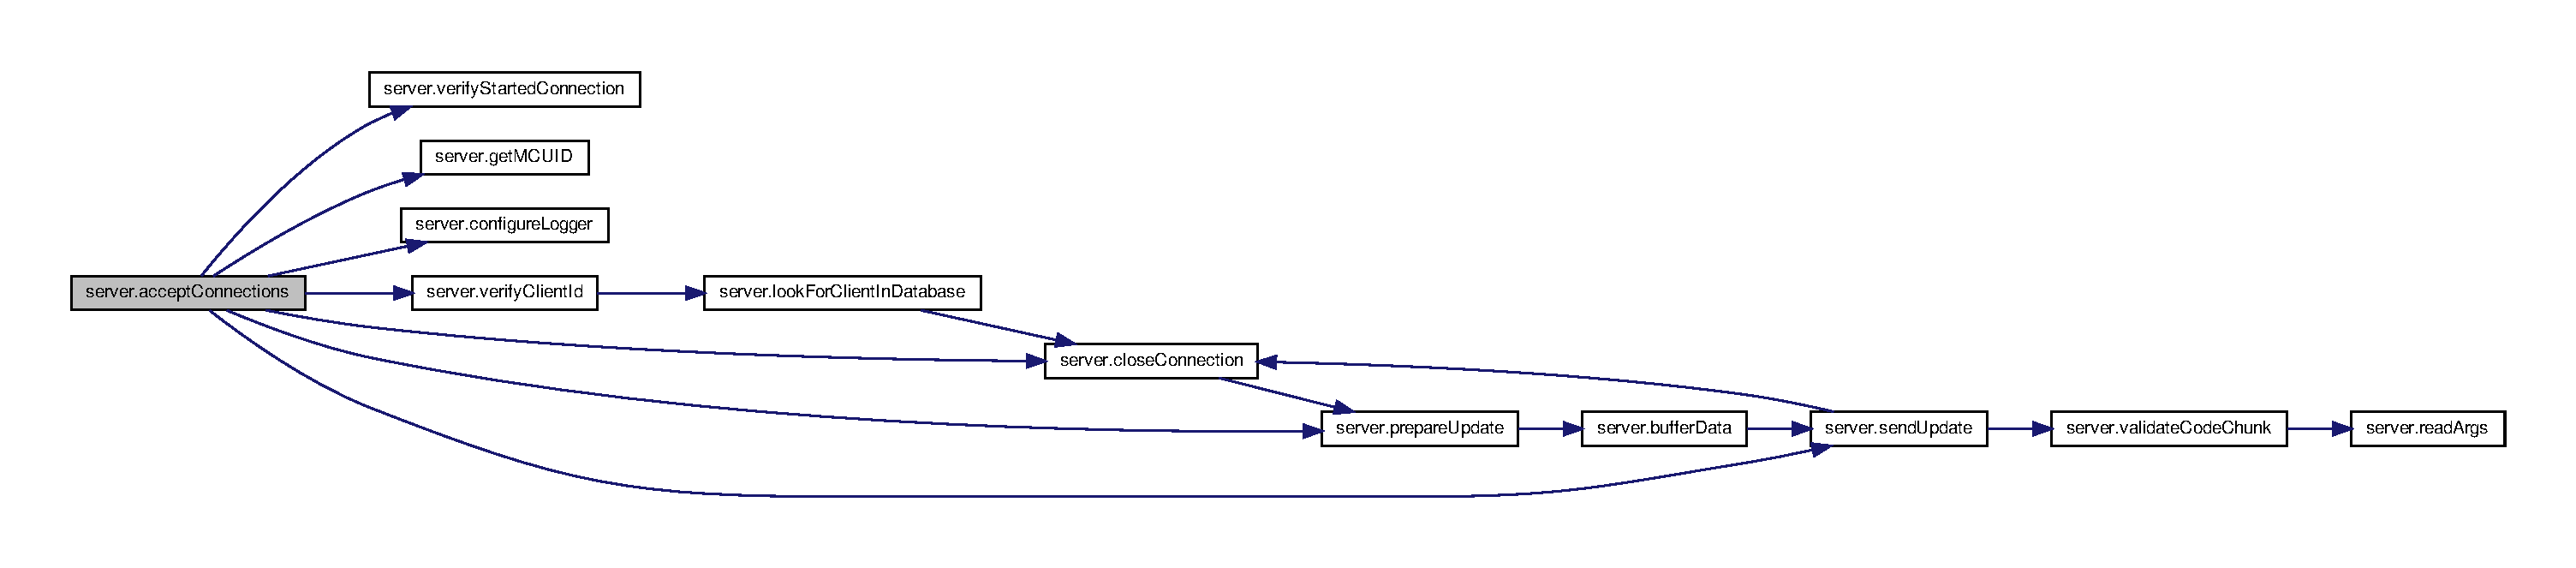
\includegraphics[width=350pt]{namespaceserver_ac1ec62c626a3425033381ef5718ce12b_cgraph}
\end{center}
\end{figure}
Here is the caller graph for this function\+:
\nopagebreak
\begin{figure}[H]
\begin{center}
\leavevmode
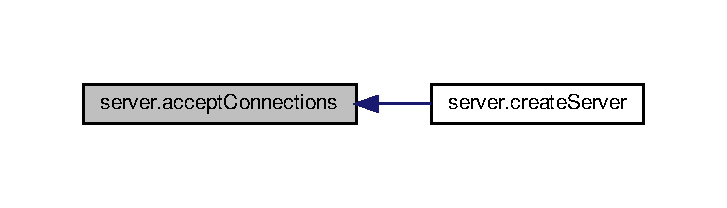
\includegraphics[width=349pt]{namespaceserver_ac1ec62c626a3425033381ef5718ce12b_icgraph}
\end{center}
\end{figure}
\mbox{\Hypertarget{namespaceserver_a6098d5cffff301a01e793c84215c4512}\label{namespaceserver_a6098d5cffff301a01e793c84215c4512}} 
\index{server@{server}!buffer\+Data@{buffer\+Data}}
\index{buffer\+Data@{buffer\+Data}!server@{server}}
\subsubsection{\texorpdfstring{buffer\+Data()}{bufferData()}}
{\footnotesize\ttfamily def server.\+buffer\+Data (\begin{DoxyParamCaption}\item[{}]{filename,  }\item[{}]{binary\+File\+Lines,  }\item[{}]{logger }\end{DoxyParamCaption})}


\begin{DoxyCode}
224 \textcolor{keyword}{def }\hyperlink{namespaceserver_a6098d5cffff301a01e793c84215c4512}{bufferData}(filename, binaryFileLines, logger):
225      countLines = 0
226      path = pathBinaryFiles+\textcolor{stringliteral}{"/"}+ filename
227      \textcolor{keywordflow}{if} (os.path.exists(path)== \textcolor{keyword}{False}):
228           logger.error(\textcolor{stringliteral}{"Required file does not exist \{\}"}.format(path))
229           \textcolor{keywordflow}{return} UNABLE\_BUFFERING\_CODE
230      with open(path, \textcolor{stringliteral}{'r') as file:}
231 \textcolor{stringliteral}{          logger.info("Opening file \{\}"}.format(path))
232           line = file.readline()
233           countLines += 1
234           \textcolor{keywordflow}{while} (line \textcolor{keywordflow}{and} countLines < bufferSizeFile):
235                line = file.readline()
236                chunk = re.findall(\textcolor{stringliteral}{r'^S1+[0-9A-F]+\(\backslash\)w|^S2+[0-9A-F]+\(\backslash\)w|^S3+[0-9A-F]+\(\backslash\)w'}, line)
237                \textcolor{keywordflow}{if} (len(chunk)>0):
238                     binaryFileLines.append(chunk[0])
239                countLines += 1
240           if(file.readline() == \textcolor{stringliteral}{''}):
241                file.close()
242                \textcolor{keywordflow}{return} SUCCESSFUL
243           file.close()
244           \textcolor{keywordflow}{return} BUFFERING\_CODE\_INCOMPLETE
245      \textcolor{keywordflow}{return} UNABLE\_BUFFERING\_CODE
246 
\end{DoxyCode}
Here is the call graph for this function\+:
\nopagebreak
\begin{figure}[H]
\begin{center}
\leavevmode
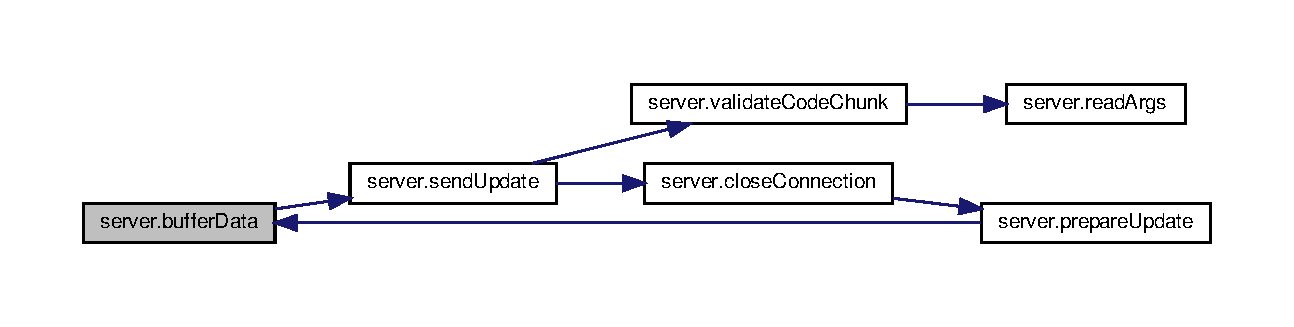
\includegraphics[width=350pt]{namespaceserver_a6098d5cffff301a01e793c84215c4512_cgraph}
\end{center}
\end{figure}
Here is the caller graph for this function\+:
\nopagebreak
\begin{figure}[H]
\begin{center}
\leavevmode
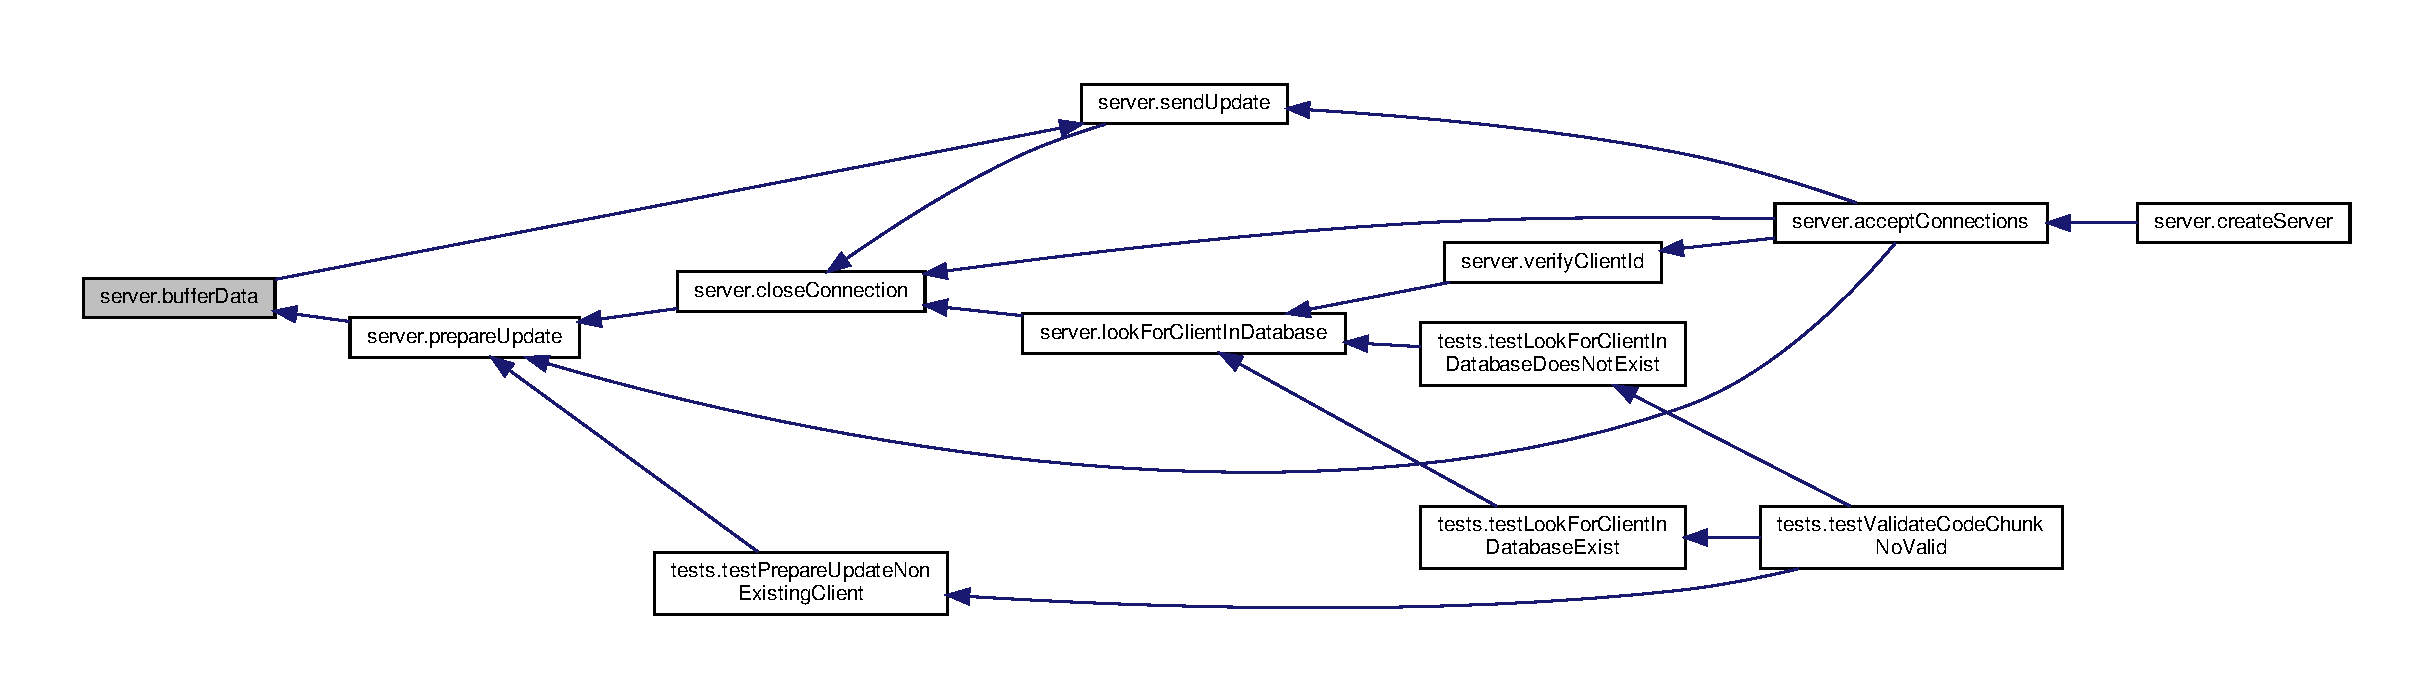
\includegraphics[width=350pt]{namespaceserver_a6098d5cffff301a01e793c84215c4512_icgraph}
\end{center}
\end{figure}
\mbox{\Hypertarget{namespaceserver_a2e99d18201fed087163454b021b7c007}\label{namespaceserver_a2e99d18201fed087163454b021b7c007}} 
\index{server@{server}!close\+Connection@{close\+Connection}}
\index{close\+Connection@{close\+Connection}!server@{server}}
\subsubsection{\texorpdfstring{close\+Connection()}{closeConnection()}}
{\footnotesize\ttfamily def server.\+close\+Connection (\begin{DoxyParamCaption}\item[{}]{connection,  }\item[{}]{logger }\end{DoxyParamCaption})}


\begin{DoxyCode}
199 \textcolor{keyword}{def }\hyperlink{namespaceserver_a2e99d18201fed087163454b021b7c007}{closeConnection}(connection, logger):
200      logger.info(\textcolor{stringliteral}{"Close of connection has been requested"})
201      connection.close()
202      \textcolor{keywordflow}{return} SUCCESSFUL
203 
\end{DoxyCode}
Here is the call graph for this function\+:
\nopagebreak
\begin{figure}[H]
\begin{center}
\leavevmode
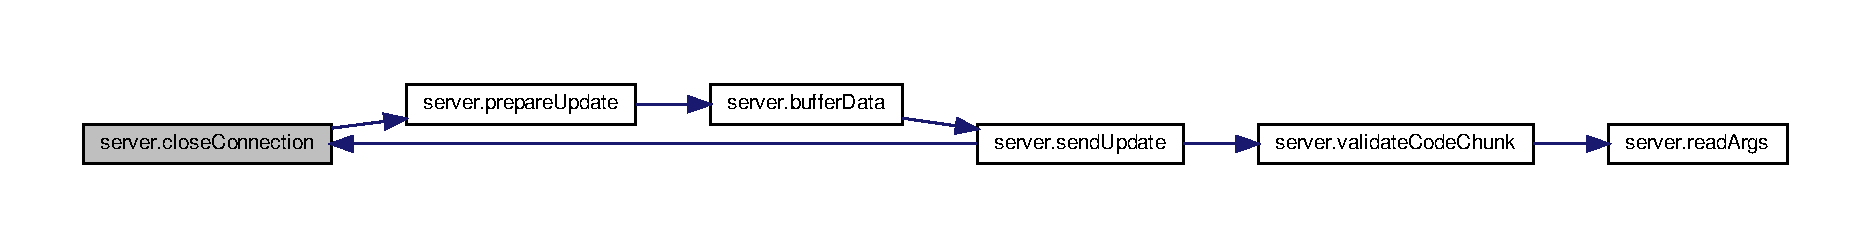
\includegraphics[width=350pt]{namespaceserver_a2e99d18201fed087163454b021b7c007_cgraph}
\end{center}
\end{figure}
Here is the caller graph for this function\+:
\nopagebreak
\begin{figure}[H]
\begin{center}
\leavevmode
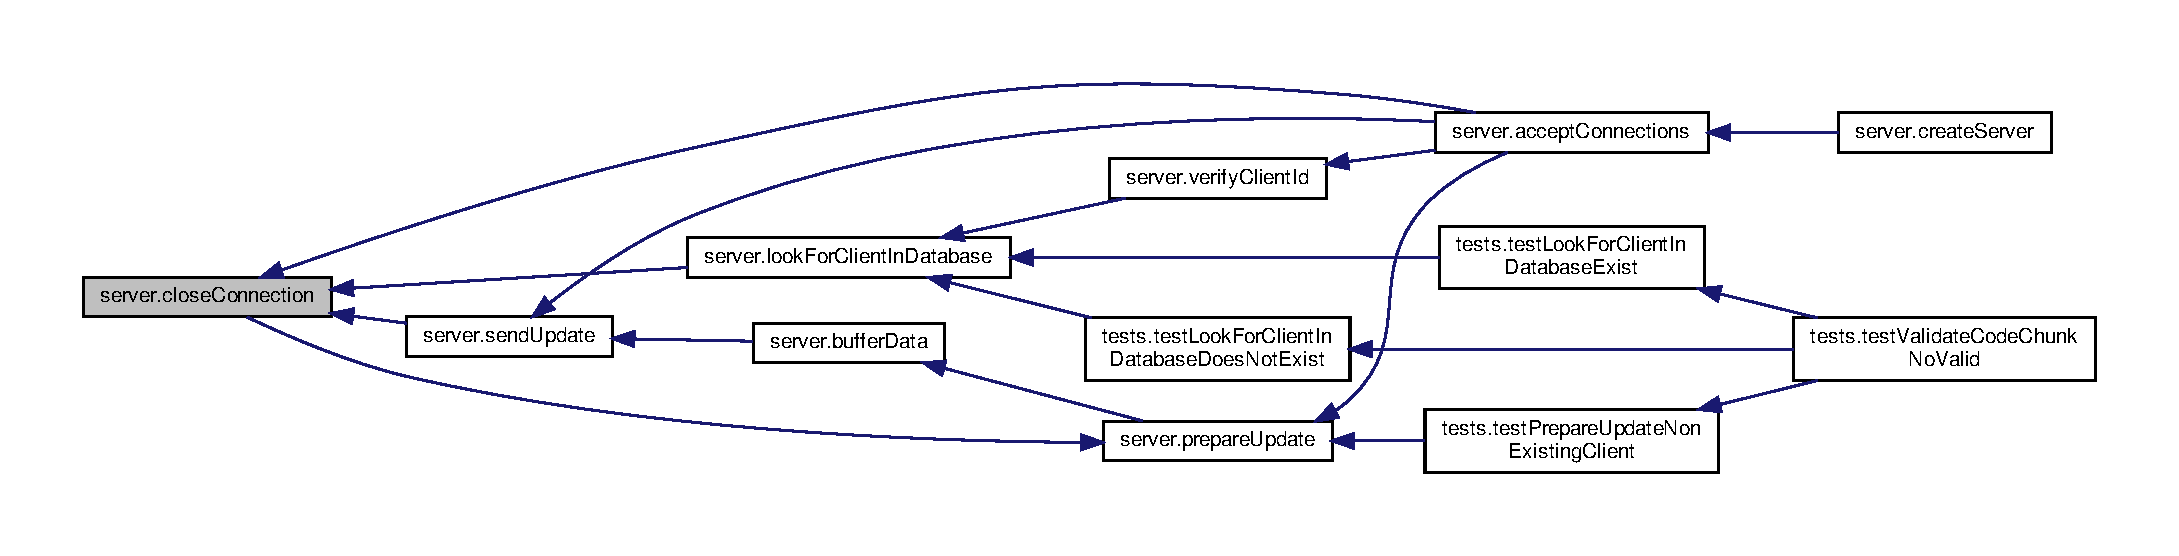
\includegraphics[width=350pt]{namespaceserver_a2e99d18201fed087163454b021b7c007_icgraph}
\end{center}
\end{figure}
\mbox{\Hypertarget{namespaceserver_a44a7428717edc164d7dd564478da2da3}\label{namespaceserver_a44a7428717edc164d7dd564478da2da3}} 
\index{server@{server}!configure\+Logger@{configure\+Logger}}
\index{configure\+Logger@{configure\+Logger}!server@{server}}
\subsubsection{\texorpdfstring{configure\+Logger()}{configureLogger()}}
{\footnotesize\ttfamily def server.\+configure\+Logger (\begin{DoxyParamCaption}\item[{}]{log\+File }\end{DoxyParamCaption})}


\begin{DoxyCode}
83 \textcolor{keyword}{def }\hyperlink{namespaceserver_a44a7428717edc164d7dd564478da2da3}{configureLogger}(logFile):
84      \textcolor{comment}{# Logger name}
85      logger = logging.getLogger(logFile)
86      \textcolor{comment}{# Set the log level to LOG\_LEVEL}
87      logger.setLevel(LOG\_LEVEL)
88      \textcolor{comment}{# Make a handler that wirtes to a file, making a new file at midnight and keeping}
89      \textcolor{comment}{# 3 backups}
90      handler = logging.handlers.TimedRotatingFileHandler(logFile, when=\textcolor{stringliteral}{"midnight"}, backupCount =3)
91      \textcolor{comment}{#Format each log message like this}
92      formatter = logging.Formatter(\textcolor{stringliteral}{'%(asctime)s %(levelname)-8s %(message)s'})
93      \textcolor{comment}{#Attach the formatter to the handler}
94      handler.setFormatter(formatter)
95      \textcolor{comment}{#Attach the handler to the logger}
96      logger.addHandler(handler)
97      \textcolor{comment}{#Replacement of stdout with loggin to file at INFO level}
98      sys.stdout = CustomLogger(logger, logging.INFO)
99      \textcolor{comment}{#Replacement of stdout with loggin to file at ERROR level}
100      sys.stderr = CustomLogger(logger, logging.ERROR)
101      \textcolor{keywordflow}{return} logger
102  
\end{DoxyCode}
Here is the caller graph for this function\+:
\nopagebreak
\begin{figure}[H]
\begin{center}
\leavevmode
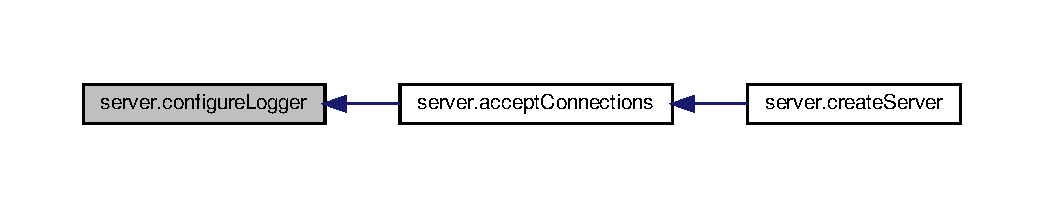
\includegraphics[width=350pt]{namespaceserver_a44a7428717edc164d7dd564478da2da3_icgraph}
\end{center}
\end{figure}
\mbox{\Hypertarget{namespaceserver_a5dce7c3abe85653dccf395dfb4f4b664}\label{namespaceserver_a5dce7c3abe85653dccf395dfb4f4b664}} 
\index{server@{server}!connect\+Socket@{connect\+Socket}}
\index{connect\+Socket@{connect\+Socket}!server@{server}}
\subsubsection{\texorpdfstring{connect\+Socket()}{connectSocket()}}
{\footnotesize\ttfamily def server.\+connect\+Socket (\begin{DoxyParamCaption}\item[{}]{socket }\end{DoxyParamCaption})}


\begin{DoxyCode}
20 \textcolor{keyword}{def }\hyperlink{namespaceserver_a5dce7c3abe85653dccf395dfb4f4b664}{connectSocket}(socket):
21      data = \textcolor{stringliteral}{""}
22      client, address = socket.accept()
23      client.settimeout(TIMEOUT)
24      data =  client.recv()
25      openConnections.append(client)
26      \textcolor{keywordflow}{if} data != \textcolor{stringliteral}{"@"}:
27           logger.debug(\textcolor{stringliteral}{"\{u\} connected"}.format(u=address))
28           client.send(\textcolor{stringliteral}{"OK"})
29      openConnections.remove()
30      client.close()
31      
32      
33 
\end{DoxyCode}
\mbox{\Hypertarget{namespaceserver_a240f07b12d57cfa5cff5612501fe7dc8}\label{namespaceserver_a240f07b12d57cfa5cff5612501fe7dc8}} 
\index{server@{server}!create\+Server@{create\+Server}}
\index{create\+Server@{create\+Server}!server@{server}}
\subsubsection{\texorpdfstring{create\+Server()}{createServer()}}
{\footnotesize\ttfamily def server.\+create\+Server (\begin{DoxyParamCaption}\item[{}]{connections\+List,  }\item[{}]{clients\+List }\end{DoxyParamCaption})}


\begin{DoxyCode}
103 \textcolor{keyword}{def }\hyperlink{namespaceserver_a240f07b12d57cfa5cff5612501fe7dc8}{createServer}(connectionsList, clientsList):
104      
107      sock = socket.socket(socket.AF\_INET, socket.SOCK\_STREAM)
108      hostname = socket.gethostname()
109      logger.info(\textcolor{stringliteral}{"Hostname \{\}"}.format(hostname))
110      \textcolor{comment}{#Cleaning previous connections}
111      sock.setsockopt(socket.SOL\_SOCKET, socket.SO\_REUSEADDR,1)
112      \textcolor{comment}{#For binding address and port}
113      \textcolor{comment}{# 0.0.0.0 because that makes our server available over any IP address}
114      sock.bind((host,port))
115      \textcolor{comment}{#Listen argument: Maximum in queue pendings}
116      sock.listen(5)
117      inputs.append(sock)
118      logger.info(\textcolor{stringliteral}{"Server ready to listen"})
119      \hyperlink{namespaceserver_ac1ec62c626a3425033381ef5718ce12b}{acceptConnections}(connectionsList, clientsList, sock, logger)
120 
\end{DoxyCode}
Here is the call graph for this function\+:
\nopagebreak
\begin{figure}[H]
\begin{center}
\leavevmode
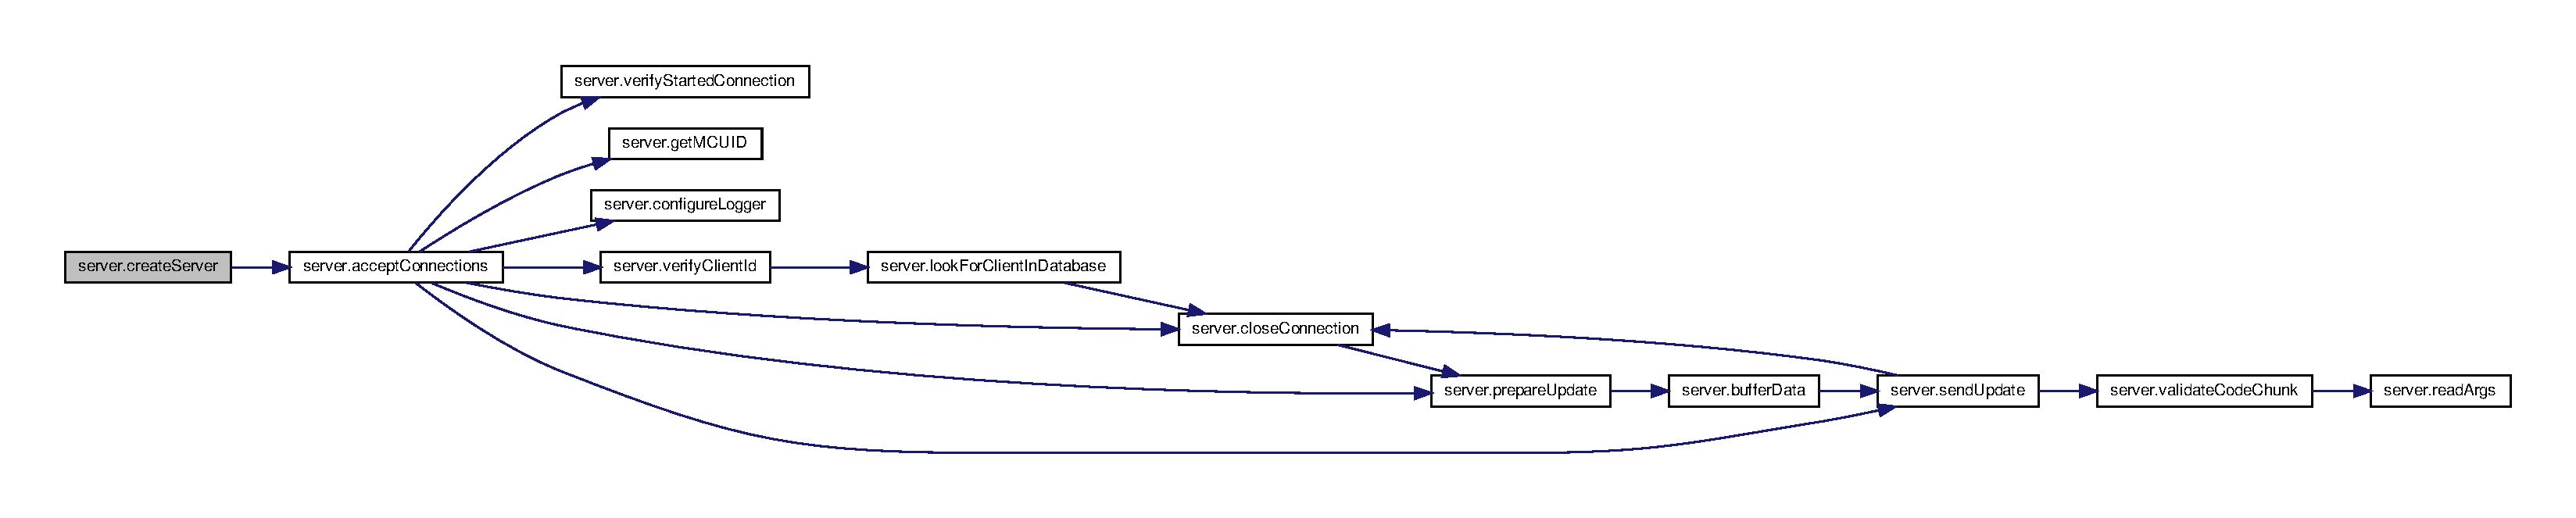
\includegraphics[width=350pt]{namespaceserver_a240f07b12d57cfa5cff5612501fe7dc8_cgraph}
\end{center}
\end{figure}
\mbox{\Hypertarget{namespaceserver_a26f3a1d49ee9e013ed77fbcb273a99be}\label{namespaceserver_a26f3a1d49ee9e013ed77fbcb273a99be}} 
\index{server@{server}!get\+M\+C\+U\+ID@{get\+M\+C\+U\+ID}}
\index{get\+M\+C\+U\+ID@{get\+M\+C\+U\+ID}!server@{server}}
\subsubsection{\texorpdfstring{get\+M\+C\+U\+I\+D()}{getMCUID()}}
{\footnotesize\ttfamily def server.\+get\+M\+C\+U\+ID (\begin{DoxyParamCaption}\item[{}]{connection,  }\item[{}]{address,  }\item[{}]{logger }\end{DoxyParamCaption})}


\begin{DoxyCode}
157 \textcolor{keyword}{def }\hyperlink{namespaceserver_a26f3a1d49ee9e013ed77fbcb273a99be}{getMCUID}(connection, address, logger):
158      receivedData = connection.recv(maxBytes)
159      logger.info(\textcolor{stringliteral}{"Server has received data from \{\}"}.format(address))
160      mcuid = re.findall(\textcolor{stringliteral}{"^\(\backslash\)@(\(\backslash\)d\{25\})[0-9]*#$"}, receivedData.decode(\textcolor{stringliteral}{"utf-8"}))
161                         
162      if(len(mcuid) == 1):
163           \textcolor{keywordflow}{return} mcuid[0]
164      \textcolor{keywordflow}{else}:
165           \textcolor{keywordflow}{return} UNFORMATTED\_MCUID
166 
\end{DoxyCode}
Here is the caller graph for this function\+:
\nopagebreak
\begin{figure}[H]
\begin{center}
\leavevmode
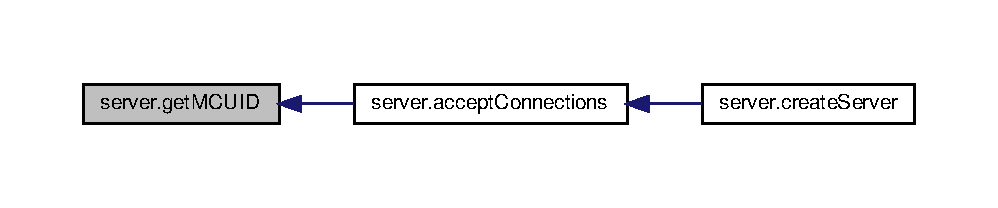
\includegraphics[width=350pt]{namespaceserver_a26f3a1d49ee9e013ed77fbcb273a99be_icgraph}
\end{center}
\end{figure}
\mbox{\Hypertarget{namespaceserver_a998e5671e2ab0c79b9abe44e87e203a0}\label{namespaceserver_a998e5671e2ab0c79b9abe44e87e203a0}} 
\index{server@{server}!look\+For\+Client\+In\+Database@{look\+For\+Client\+In\+Database}}
\index{look\+For\+Client\+In\+Database@{look\+For\+Client\+In\+Database}!server@{server}}
\subsubsection{\texorpdfstring{look\+For\+Client\+In\+Database()}{lookForClientInDatabase()}}
{\footnotesize\ttfamily def server.\+look\+For\+Client\+In\+Database (\begin{DoxyParamCaption}\item[{}]{mcuid,  }\item[{}]{logger }\end{DoxyParamCaption})}


\begin{DoxyCode}
179 \textcolor{keyword}{def }\hyperlink{namespaceserver_a998e5671e2ab0c79b9abe44e87e203a0}{lookForClientInDatabase}(mcuid, logger):
180      
181      clientInfo = []
182      logger.info(\textcolor{stringliteral}{"Opening file \{\}, to verify MCUID \{\}"}.format(databaseName,mcuid))
183      \textcolor{keywordflow}{try}:
184           with open(databaseName, \textcolor{stringliteral}{'r') as file:               }\textcolor{keywordflow}{for} line \textcolor{keywordflow}{in} file:
185                     clientInfo = line.split(\textcolor{stringliteral}{','})
186                     \textcolor{keywordflow}{if} (len(clientInfo) == 3):
187                          \textcolor{keywordflow}{if} (clientInfo[0] == mcuid):
188                              \textcolor{keywordflow}{return} SUCCESSFUL, clientInfo
189                          \textcolor{keywordflow}{else}:
190                               \textcolor{keywordflow}{continue}
191                     \textcolor{keywordflow}{else}:
192                          \textcolor{keywordflow}{return} UNPROPER\_FILE\_FORMAT, clientInfo
193           file.close()
194      \textcolor{keywordflow}{except}:
195           logger.error(\textcolor{stringliteral}{"Error opening file"})
196      \textcolor{keywordflow}{return} CLIENT\_UNVERIFIED, clientInfo
197 
198 \end{DoxyCode}
Here is the call graph for this function\+:
\nopagebreak
\begin{figure}[H]
\begin{center}
\leavevmode
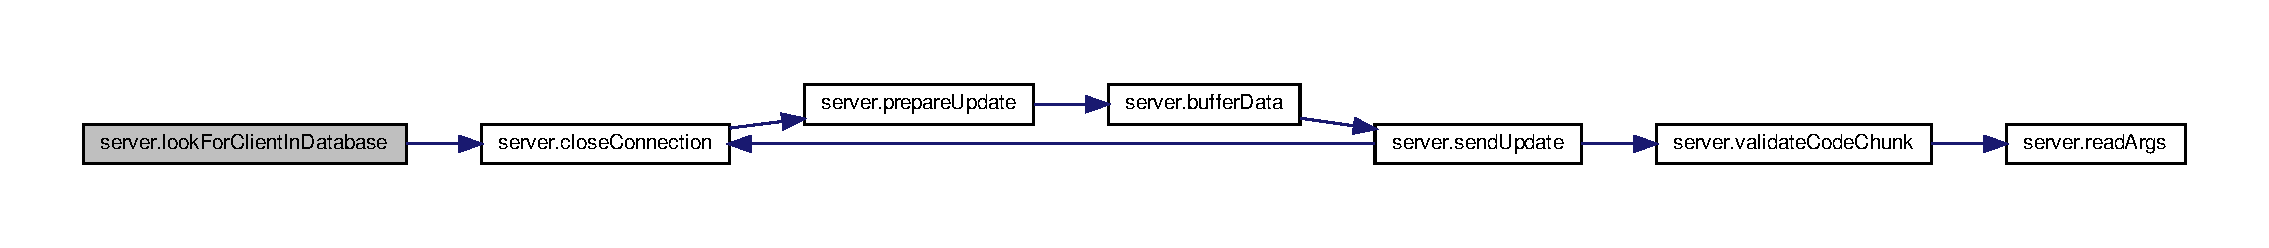
\includegraphics[width=350pt]{namespaceserver_a998e5671e2ab0c79b9abe44e87e203a0_cgraph}
\end{center}
\end{figure}
Here is the caller graph for this function\+:
\nopagebreak
\begin{figure}[H]
\begin{center}
\leavevmode
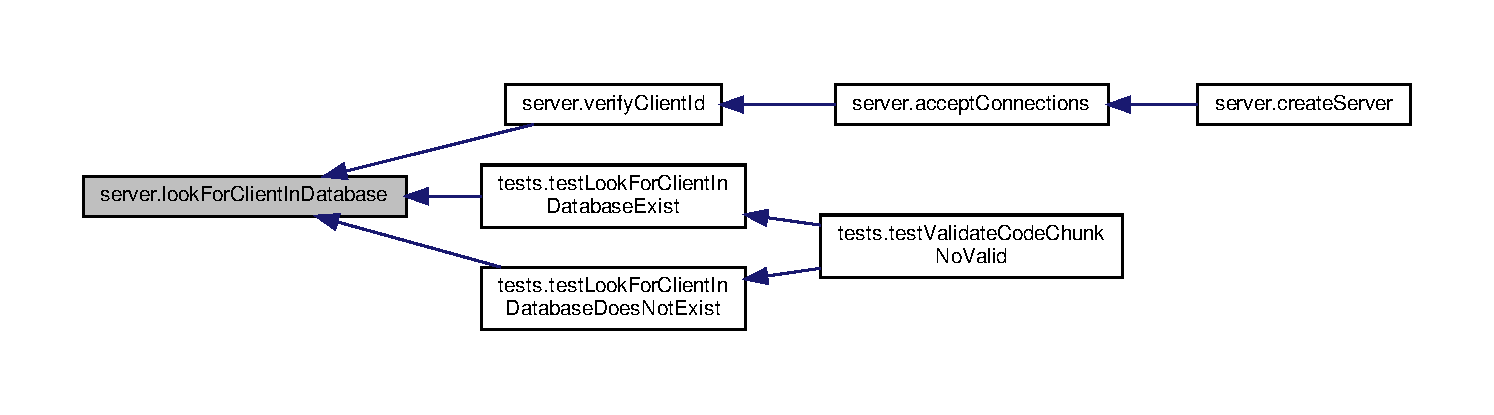
\includegraphics[width=350pt]{namespaceserver_a998e5671e2ab0c79b9abe44e87e203a0_icgraph}
\end{center}
\end{figure}
\mbox{\Hypertarget{namespaceserver_a4ab7e63c5f934dfea50b006468f9efca}\label{namespaceserver_a4ab7e63c5f934dfea50b006468f9efca}} 
\index{server@{server}!prepare\+Update@{prepare\+Update}}
\index{prepare\+Update@{prepare\+Update}!server@{server}}
\subsubsection{\texorpdfstring{prepare\+Update()}{prepareUpdate()}}
{\footnotesize\ttfamily def server.\+prepare\+Update (\begin{DoxyParamCaption}\item[{}]{client\+Info,  }\item[{}]{clients\+List,  }\item[{}]{logger }\end{DoxyParamCaption})}


\begin{DoxyCode}
204 \textcolor{keyword}{def }\hyperlink{namespaceserver_a4ab7e63c5f934dfea50b006468f9efca}{prepareUpdate}(clientInfo, clientsList, logger):
205      logger.info(\textcolor{stringliteral}{"Preparing update for \{\}"}.format(clientInfo))
206      \textcolor{comment}{#Buffer data from file to be sent to specific client}
207      binaryFileLines = []
208      bufferingStatus = \hyperlink{namespaceserver_a6098d5cffff301a01e793c84215c4512}{bufferData}(clientInfo[1], binaryFileLines, logger)
209      logger.info(\textcolor{stringliteral}{"Status prepare update \{\}"}.format(bufferingStatus))
210      \textcolor{keywordflow}{if} (bufferingStatus == SUCCESSFUL):
211           FWVersion = re.findall(\textcolor{stringliteral}{r"([0-9A-F]+)"}, clientInfo[2])
212           binaryFileLines.append(\textcolor{stringliteral}{"@\{\}##"}.format(FWVersion[0]))
213           logger.info(\textcolor{stringliteral}{"Buffered code \{\}"}.format(binaryFileLines))
214           logger.info(\textcolor{stringliteral}{"Code buffer done successfully"}) 
215           clientsList.append(\{\textcolor{stringliteral}{"mcuid"}:clientInfo[0], \textcolor{stringliteral}{"filename"}:clientInfo[1], \textcolor{stringliteral}{"codelines"}: binaryFileLines
      , \textcolor{stringliteral}{"status"}: READY\_TO\_UPDATE\})                 
216           \textcolor{keywordflow}{return} SUCCESSFUL
217      \textcolor{keywordflow}{if} (bufferingStatus == BUFFERING\_CODE\_INCOMPLETE):
218           
219           logger.info(\textcolor{stringliteral}{"Incomplete buffering code"})
220           \textcolor{keywordflow}{return} BUFFERING\_CODE\_INCOMPLETE
221      \textcolor{keywordflow}{else}:
222           \textcolor{keywordflow}{return} UNABLE\_BUFFERING\_CODE
223 
\end{DoxyCode}
Here is the call graph for this function\+:
\nopagebreak
\begin{figure}[H]
\begin{center}
\leavevmode
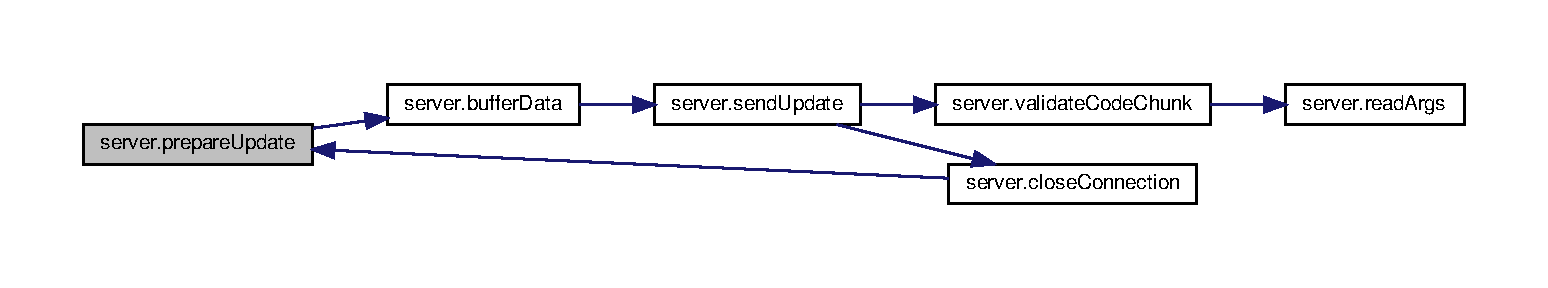
\includegraphics[width=350pt]{namespaceserver_a4ab7e63c5f934dfea50b006468f9efca_cgraph}
\end{center}
\end{figure}
Here is the caller graph for this function\+:
\nopagebreak
\begin{figure}[H]
\begin{center}
\leavevmode
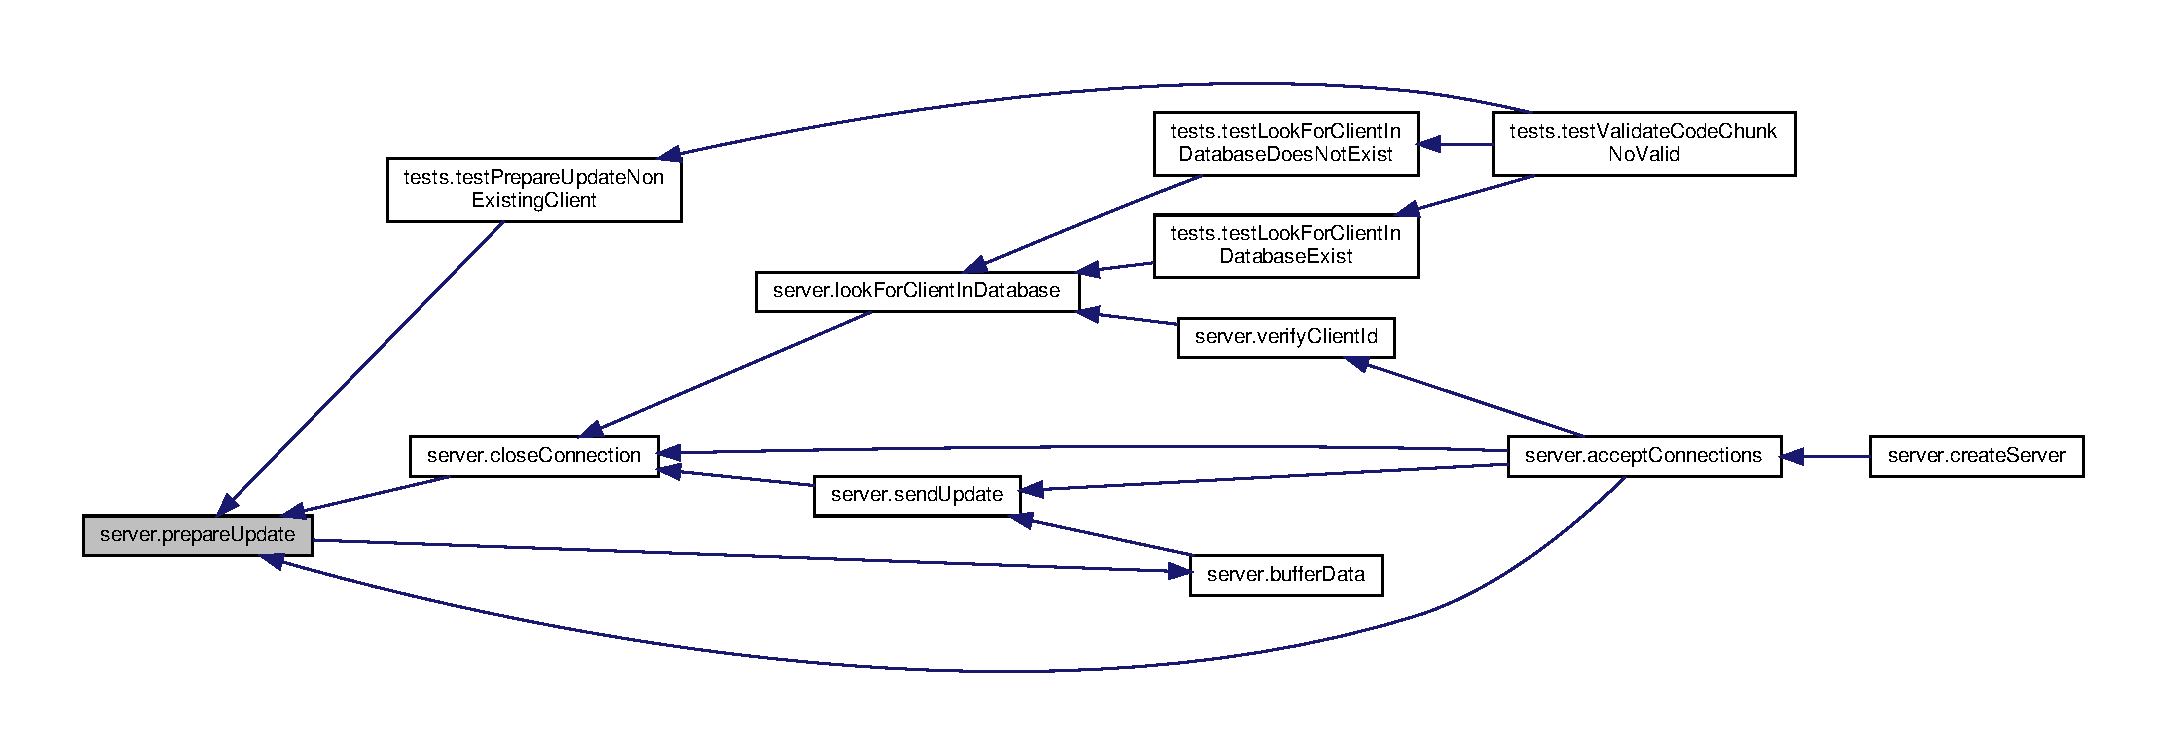
\includegraphics[width=350pt]{namespaceserver_a4ab7e63c5f934dfea50b006468f9efca_icgraph}
\end{center}
\end{figure}
\mbox{\Hypertarget{namespaceserver_aa317dc86338d02253076787cc8e5d997}\label{namespaceserver_aa317dc86338d02253076787cc8e5d997}} 
\index{server@{server}!read\+Args@{read\+Args}}
\index{read\+Args@{read\+Args}!server@{server}}
\subsubsection{\texorpdfstring{read\+Args()}{readArgs()}}
{\footnotesize\ttfamily def server.\+read\+Args (\begin{DoxyParamCaption}{ }\end{DoxyParamCaption})}


\begin{DoxyCode}
73 \textcolor{keyword}{def }\hyperlink{namespaceserver_aa317dc86338d02253076787cc8e5d997}{readArgs}():
74      parser = argparse.ArgumentParser(description=\textcolor{stringliteral}{"OTA server in python"})
75      parser.add\_argument(\textcolor{stringliteral}{"-db"}, \textcolor{stringliteral}{"--dbname"}, help=\textcolor{stringliteral}{"Database file name (path included)"}, default=
      PATH\_DATABASE\_DEFAULT)
76      parser.add\_argument(\textcolor{stringliteral}{"-pbf"}, \textcolor{stringliteral}{"--pathbinaryfiles"}, help=\textcolor{stringliteral}{"Binary files path"}, default=
      PATH\_BINARY\_FILE\_DEFAULT)
77      parser.add\_argument(\textcolor{stringliteral}{"-ho"}, \textcolor{stringliteral}{"--host"}, help=\textcolor{stringliteral}{"Host IP"}, default=HOST\_DEFAULT)
78      parser.add\_argument(\textcolor{stringliteral}{"-p"}, \textcolor{stringliteral}{"--port"}, help=\textcolor{stringliteral}{"Port to establish communication"}, default=PORT\_DEFAULT)
79      parser.add\_argument(\textcolor{stringliteral}{"-lp"}, \textcolor{stringliteral}{"--logpath"}, help=\textcolor{stringliteral}{"Path to save logging"}, default=LOG\_PATH\_DEFAULT)
80      args = parser.parse\_args()
81      \textcolor{keywordflow}{return} args
82 
\end{DoxyCode}
Here is the caller graph for this function\+:
\nopagebreak
\begin{figure}[H]
\begin{center}
\leavevmode
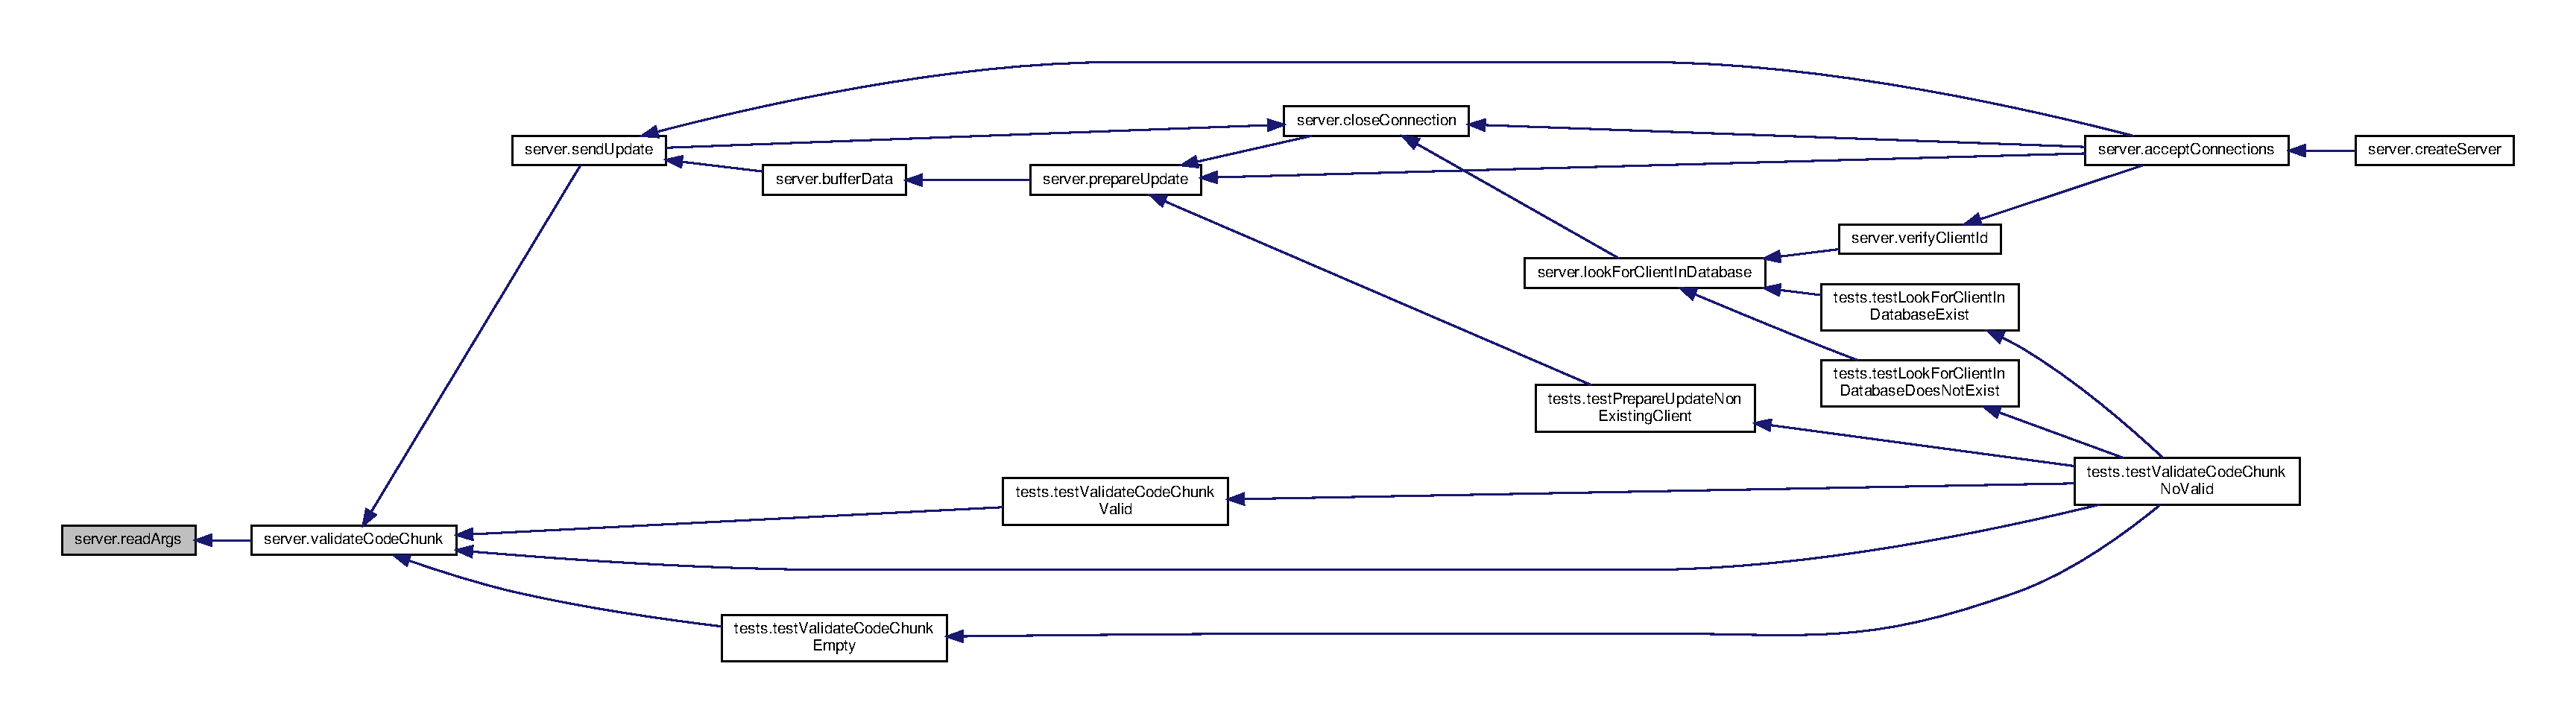
\includegraphics[width=350pt]{namespaceserver_aa317dc86338d02253076787cc8e5d997_icgraph}
\end{center}
\end{figure}
\mbox{\Hypertarget{namespaceserver_a4889d0db3f3503cc61340252fabc2c24}\label{namespaceserver_a4889d0db3f3503cc61340252fabc2c24}} 
\index{server@{server}!send\+Update@{send\+Update}}
\index{send\+Update@{send\+Update}!server@{server}}
\subsubsection{\texorpdfstring{send\+Update()}{sendUpdate()}}
{\footnotesize\ttfamily def server.\+send\+Update (\begin{DoxyParamCaption}\item[{}]{connection,  }\item[{}]{address,  }\item[{}]{mcuid,  }\item[{}]{client\+To\+Update,  }\item[{}]{sock,  }\item[{}]{logger }\end{DoxyParamCaption})}


\begin{DoxyCode}
247 \textcolor{keyword}{def }\hyperlink{namespaceserver_a4889d0db3f3503cc61340252fabc2c24}{sendUpdate}(connection, address, mcuid, clientToUpdate, sock, logger):
248      sock.settimeout(TIMEOUT)
249      \textcolor{keywordflow}{for} codechunk \textcolor{keywordflow}{in} clientToUpdate[0][\textcolor{stringliteral}{'codelines'}]:
250           \textcolor{keywordflow}{if} (\hyperlink{namespaceserver_ad6f5a9a8c8e233d0537dc69dc6de98f6}{validateCodeChunk}(codechunk) == SUCCESSFUL):
251                logger.info(\textcolor{stringliteral}{"Data from server \{\}"}.format(codechunk))
252                \textcolor{keywordflow}{try}:
253                     connection.send(codechunk.encode())
254                     receivedData = connection.recv(1024)
255                     logger.info(\textcolor{stringliteral}{"Data from client: \{\}"}.format(receivedData))
256                     \textcolor{keywordflow}{if} (receivedData == ackClient):
257                          \textcolor{keywordflow}{continue}
258                     \textcolor{keywordflow}{else}:
259                          \hyperlink{namespaceserver_a2e99d18201fed087163454b021b7c007}{closeConnection}()
260                          \textcolor{keywordflow}{return} TIMEOUT\_CONNECTION
261                \textcolor{keywordflow}{except} socket.timeout \textcolor{keyword}{as} e:
262                          logger.error(\textcolor{stringliteral}{"Timeout exceed \{\}"}.format(e))
263                \textcolor{keywordflow}{except} socket.error \textcolor{keyword}{as} e:
264                     logger.error(\textcolor{stringliteral}{"Error receiving data: \{\}"}.format(e))
265                     
266           \textcolor{keywordflow}{else}:
267                \textcolor{keywordflow}{continue} 
268      logger.info(\textcolor{stringliteral}{"Update finished"})
269      \hyperlink{namespaceserver_a2e99d18201fed087163454b021b7c007}{closeConnection}(connection, logger)
270      sock.setblocking(0)
271      \textcolor{keywordflow}{return} SUCCESSFUL
272 
\end{DoxyCode}
Here is the call graph for this function\+:
\nopagebreak
\begin{figure}[H]
\begin{center}
\leavevmode
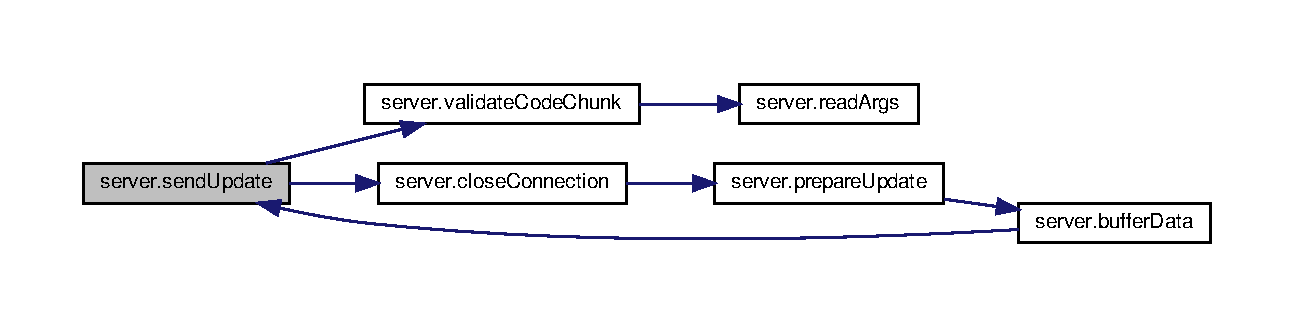
\includegraphics[width=350pt]{namespaceserver_a4889d0db3f3503cc61340252fabc2c24_cgraph}
\end{center}
\end{figure}
Here is the caller graph for this function\+:
\nopagebreak
\begin{figure}[H]
\begin{center}
\leavevmode
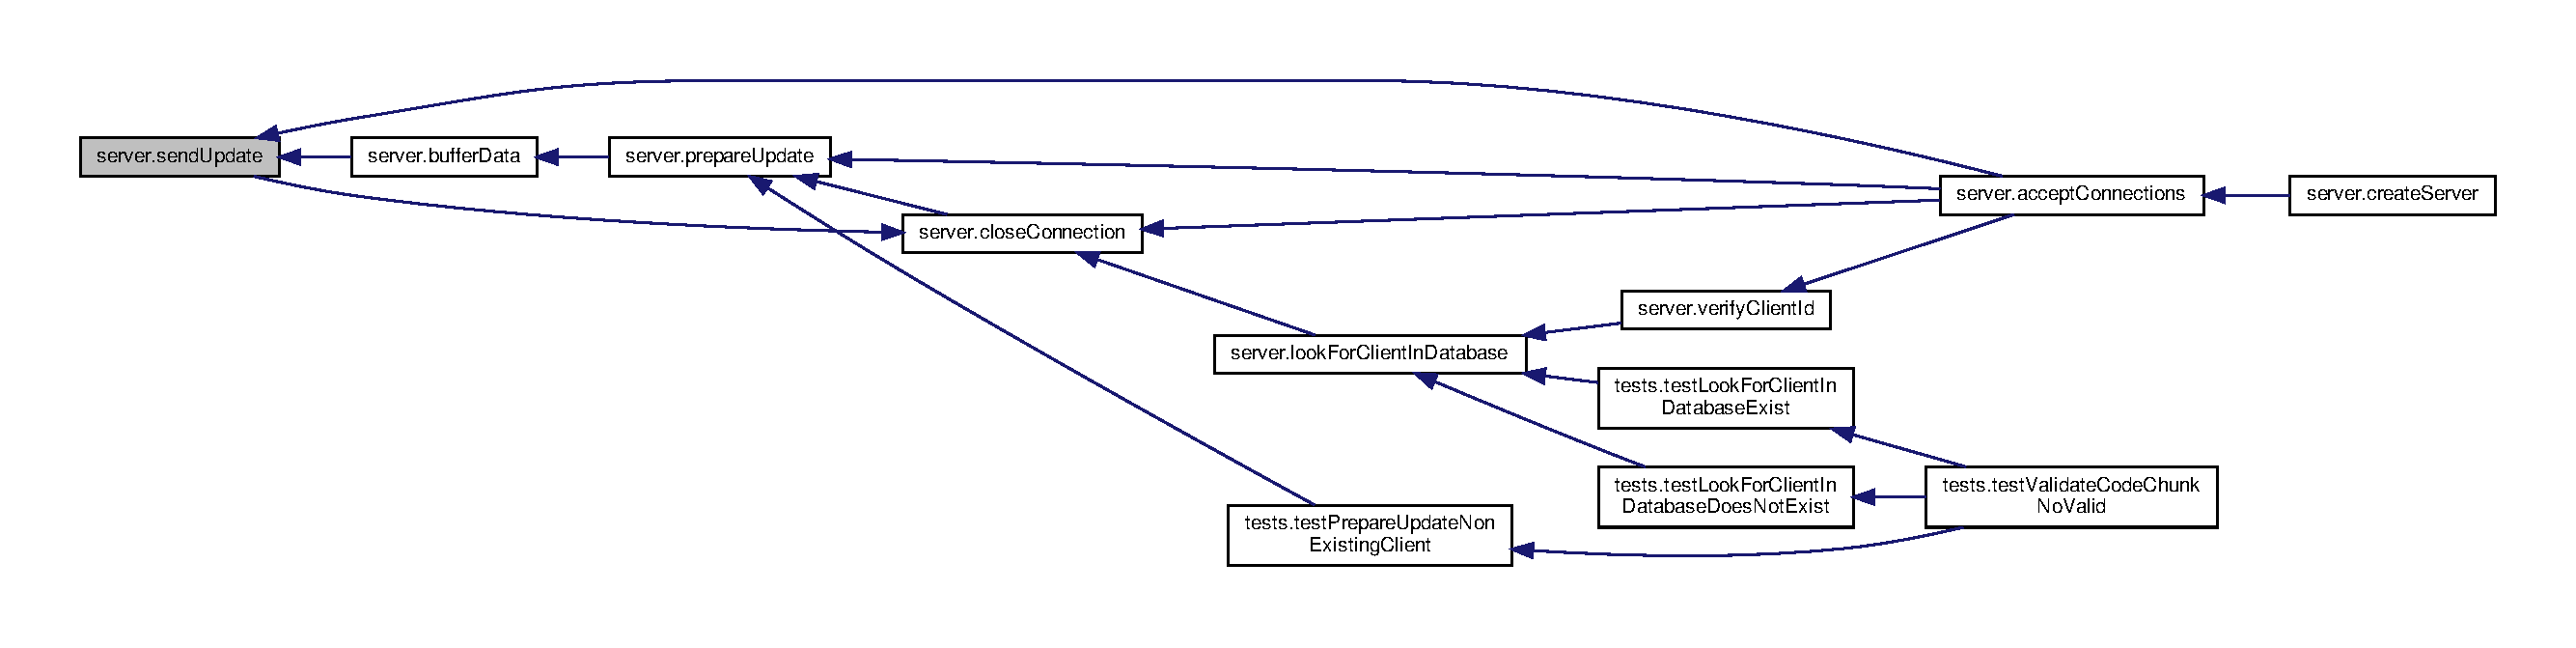
\includegraphics[width=350pt]{namespaceserver_a4889d0db3f3503cc61340252fabc2c24_icgraph}
\end{center}
\end{figure}
\mbox{\Hypertarget{namespaceserver_ad6f5a9a8c8e233d0537dc69dc6de98f6}\label{namespaceserver_ad6f5a9a8c8e233d0537dc69dc6de98f6}} 
\index{server@{server}!validate\+Code\+Chunk@{validate\+Code\+Chunk}}
\index{validate\+Code\+Chunk@{validate\+Code\+Chunk}!server@{server}}
\subsubsection{\texorpdfstring{validate\+Code\+Chunk()}{validateCodeChunk()}}
{\footnotesize\ttfamily def server.\+validate\+Code\+Chunk (\begin{DoxyParamCaption}\item[{}]{codechunk }\end{DoxyParamCaption})}


\begin{DoxyCode}
273 \textcolor{keyword}{def  }\hyperlink{namespaceserver_ad6f5a9a8c8e233d0537dc69dc6de98f6}{validateCodeChunk}(codechunk):
274      match1 = re.search(\textcolor{stringliteral}{r'^S1+[0-9A-F]+\(\backslash\)w|^S2+[0-9A-F]+\(\backslash\)w|^S3+[0-9A-F]+\(\backslash\)w'}, codechunk)
275      match2 = re.search(\textcolor{stringliteral}{r'^@([0-9A-F]\{1,2\})##$'}, codechunk)
276      \textcolor{keywordflow}{if} match1 \textcolor{keywordflow}{or} match2:
277           \textcolor{keywordflow}{return} SUCCESSFUL
278      \textcolor{keywordflow}{else}:
279           \textcolor{keywordflow}{return} INVALID\_CODE\_CHUNK
280      
\end{DoxyCode}
Here is the call graph for this function\+:
\nopagebreak
\begin{figure}[H]
\begin{center}
\leavevmode
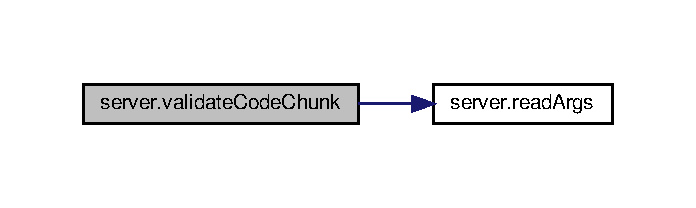
\includegraphics[width=334pt]{namespaceserver_ad6f5a9a8c8e233d0537dc69dc6de98f6_cgraph}
\end{center}
\end{figure}
Here is the caller graph for this function\+:
\nopagebreak
\begin{figure}[H]
\begin{center}
\leavevmode
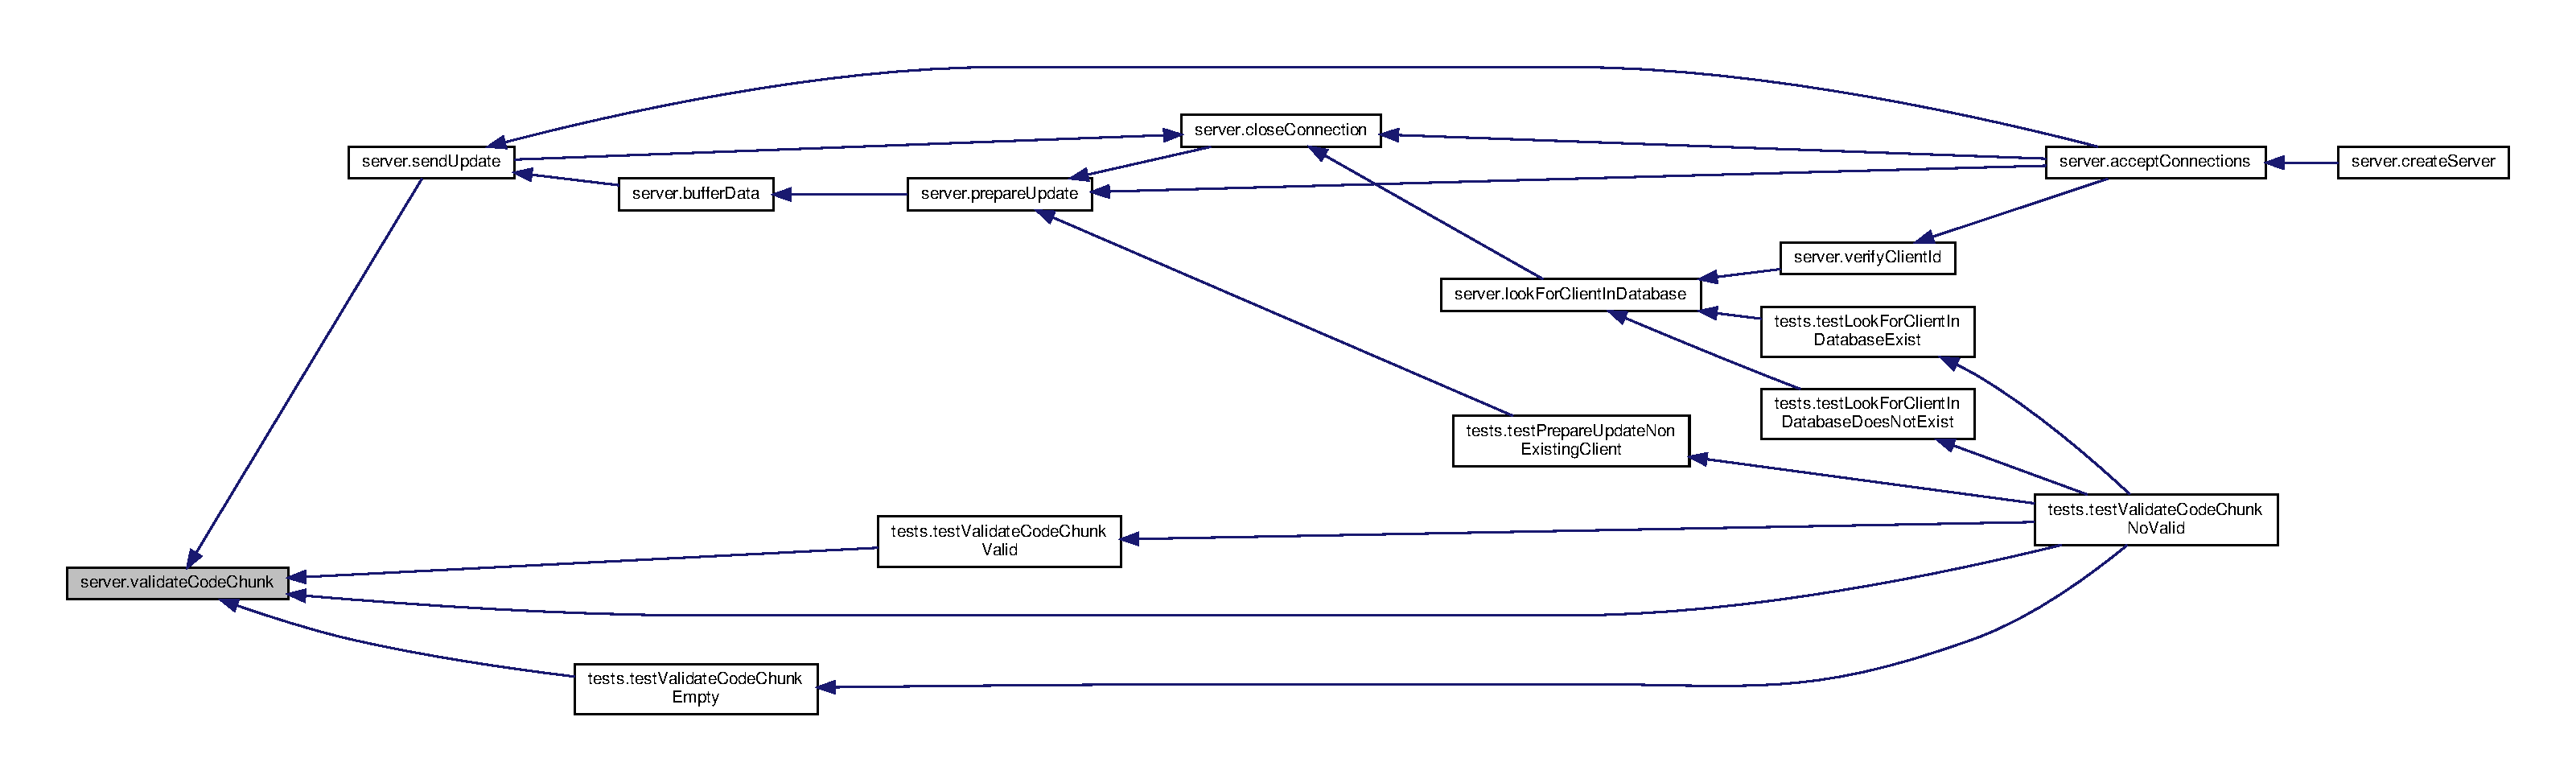
\includegraphics[width=350pt]{namespaceserver_ad6f5a9a8c8e233d0537dc69dc6de98f6_icgraph}
\end{center}
\end{figure}
\mbox{\Hypertarget{namespaceserver_a4c51be10ba9f982375f4c0a426078a96}\label{namespaceserver_a4c51be10ba9f982375f4c0a426078a96}} 
\index{server@{server}!verify\+Client\+Id@{verify\+Client\+Id}}
\index{verify\+Client\+Id@{verify\+Client\+Id}!server@{server}}
\subsubsection{\texorpdfstring{verify\+Client\+Id()}{verifyClientId()}}
{\footnotesize\ttfamily def server.\+verify\+Client\+Id (\begin{DoxyParamCaption}\item[{}]{connection,  }\item[{}]{mcuid,  }\item[{}]{logger }\end{DoxyParamCaption})}


\begin{DoxyCode}
167 \textcolor{keyword}{def }\hyperlink{namespaceserver_a4c51be10ba9f982375f4c0a426078a96}{verifyClientId}(connection, mcuid, logger):
168      
169      clientInfo = []
170      statusClient, clientInfo = \hyperlink{namespaceserver_a998e5671e2ab0c79b9abe44e87e203a0}{lookForClientInDatabase}(mcuid, logger)
171      if(statusClient== SUCCESSFUL):
172           logger.info(\textcolor{stringliteral}{"Client Info \{\}"}.format(clientInfo))
173           logger.info(\textcolor{stringliteral}{"Client \{\} exists in database"}.format(mcuid))
174           \textcolor{keywordflow}{return} SUCCESSFUL, clientInfo
175      \textcolor{keywordflow}{else}:
176           logger.error(\textcolor{stringliteral}{"Client \{\} does not exist in database"}.format(mcuid))
177           \textcolor{keywordflow}{return} CLIENT\_UNVERIFIED, clientInfo
178                    
\end{DoxyCode}
Here is the call graph for this function\+:
\nopagebreak
\begin{figure}[H]
\begin{center}
\leavevmode
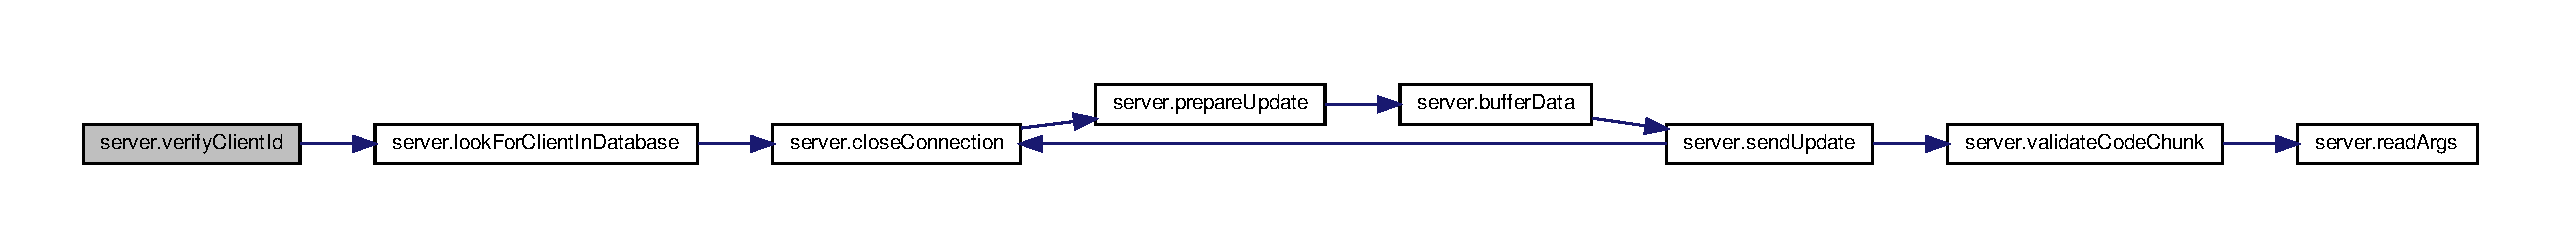
\includegraphics[width=350pt]{namespaceserver_a4c51be10ba9f982375f4c0a426078a96_cgraph}
\end{center}
\end{figure}
Here is the caller graph for this function\+:
\nopagebreak
\begin{figure}[H]
\begin{center}
\leavevmode
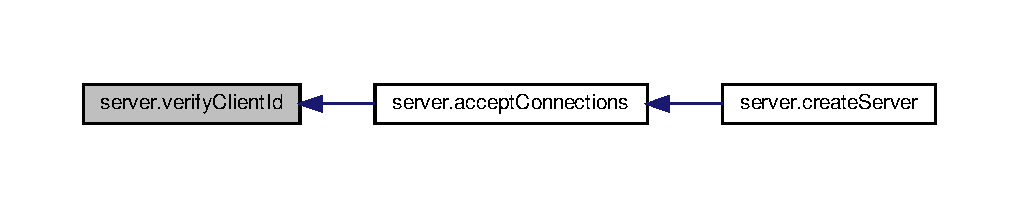
\includegraphics[width=350pt]{namespaceserver_a4c51be10ba9f982375f4c0a426078a96_icgraph}
\end{center}
\end{figure}
\mbox{\Hypertarget{namespaceserver_a4e6504daf55d2ef34d4d2ea5b30074f3}\label{namespaceserver_a4e6504daf55d2ef34d4d2ea5b30074f3}} 
\index{server@{server}!verify\+Started\+Connection@{verify\+Started\+Connection}}
\index{verify\+Started\+Connection@{verify\+Started\+Connection}!server@{server}}
\subsubsection{\texorpdfstring{verify\+Started\+Connection()}{verifyStartedConnection()}}
{\footnotesize\ttfamily def server.\+verify\+Started\+Connection (\begin{DoxyParamCaption}\item[{}]{connections,  }\item[{}]{connection }\end{DoxyParamCaption})}


\begin{DoxyCode}
150 \textcolor{keyword}{def }\hyperlink{namespaceserver_a4e6504daf55d2ef34d4d2ea5b30074f3}{verifyStartedConnection}(connections, connection):
151      \textcolor{keywordflow}{for} conn \textcolor{keywordflow}{in} connections:
152           if(conn == connection):
153                \textcolor{keywordflow}{return} ALREADY\_STARTED\_CONNECTION
154      connections.append(connection)
155      \textcolor{keywordflow}{return} NOT\_STARTED\_CONNECTION
156 
\end{DoxyCode}
Here is the caller graph for this function\+:
\nopagebreak
\begin{figure}[H]
\begin{center}
\leavevmode
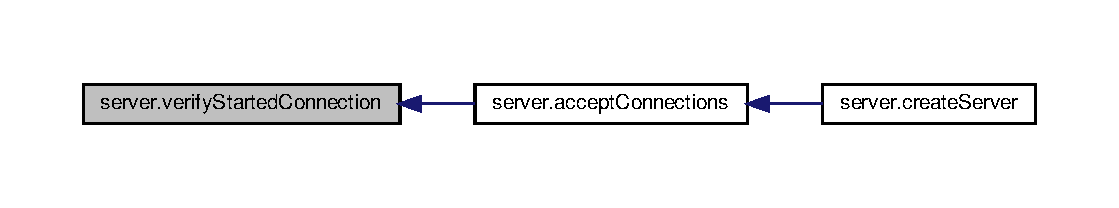
\includegraphics[width=350pt]{namespaceserver_a4e6504daf55d2ef34d4d2ea5b30074f3_icgraph}
\end{center}
\end{figure}


\subsection{Variable Documentation}
\mbox{\Hypertarget{namespaceserver_ad00458dfe9ab743680203b756f8345bf}\label{namespaceserver_ad00458dfe9ab743680203b756f8345bf}} 
\index{server@{server}!ack\+Client@{ack\+Client}}
\index{ack\+Client@{ack\+Client}!server@{server}}
\subsubsection{\texorpdfstring{ack\+Client}{ackClient}}
{\footnotesize\ttfamily string server.\+ack\+Client = b\textquotesingle{}@\textquotesingle{}}

\mbox{\Hypertarget{namespaceserver_a097162d68fd6d2855bf5eb81507db414}\label{namespaceserver_a097162d68fd6d2855bf5eb81507db414}} 
\index{server@{server}!allowed\+Update@{allowed\+Update}}
\index{allowed\+Update@{allowed\+Update}!server@{server}}
\subsubsection{\texorpdfstring{allowed\+Update}{allowedUpdate}}
{\footnotesize\ttfamily string server.\+allowed\+Update = b\textquotesingle{}@4\#\textquotesingle{}}

\mbox{\Hypertarget{namespaceserver_a02bffbe3ff309c8cca6cfdc9fe84b335}\label{namespaceserver_a02bffbe3ff309c8cca6cfdc9fe84b335}} 
\index{server@{server}!A\+L\+R\+E\+A\+D\+Y\+\_\+\+S\+T\+A\+R\+T\+E\+D\+\_\+\+C\+O\+N\+N\+E\+C\+T\+I\+ON@{A\+L\+R\+E\+A\+D\+Y\+\_\+\+S\+T\+A\+R\+T\+E\+D\+\_\+\+C\+O\+N\+N\+E\+C\+T\+I\+ON}}
\index{A\+L\+R\+E\+A\+D\+Y\+\_\+\+S\+T\+A\+R\+T\+E\+D\+\_\+\+C\+O\+N\+N\+E\+C\+T\+I\+ON@{A\+L\+R\+E\+A\+D\+Y\+\_\+\+S\+T\+A\+R\+T\+E\+D\+\_\+\+C\+O\+N\+N\+E\+C\+T\+I\+ON}!server@{server}}
\subsubsection{\texorpdfstring{A\+L\+R\+E\+A\+D\+Y\+\_\+\+S\+T\+A\+R\+T\+E\+D\+\_\+\+C\+O\+N\+N\+E\+C\+T\+I\+ON}{ALREADY\_STARTED\_CONNECTION}}
{\footnotesize\ttfamily int server.\+A\+L\+R\+E\+A\+D\+Y\+\_\+\+S\+T\+A\+R\+T\+E\+D\+\_\+\+C\+O\+N\+N\+E\+C\+T\+I\+ON = 4}

\mbox{\Hypertarget{namespaceserver_aea7e1efc19535ee9bab8400a812b43a9}\label{namespaceserver_aea7e1efc19535ee9bab8400a812b43a9}} 
\index{server@{server}!args@{args}}
\index{args@{args}!server@{server}}
\subsubsection{\texorpdfstring{args}{args}}
{\footnotesize\ttfamily server.\+args = \hyperlink{namespaceserver_aa317dc86338d02253076787cc8e5d997}{read\+Args}()}

\mbox{\Hypertarget{namespaceserver_ae86ca5f489b3b8161c0ab91cbef0d8e6}\label{namespaceserver_ae86ca5f489b3b8161c0ab91cbef0d8e6}} 
\index{server@{server}!banned\+Update@{banned\+Update}}
\index{banned\+Update@{banned\+Update}!server@{server}}
\subsubsection{\texorpdfstring{banned\+Update}{bannedUpdate}}
{\footnotesize\ttfamily string server.\+banned\+Update = b\textquotesingle{}@0\#\textquotesingle{}}

\mbox{\Hypertarget{namespaceserver_aabc8079ca922bed2eba00ad2cbc5d354}\label{namespaceserver_aabc8079ca922bed2eba00ad2cbc5d354}} 
\index{server@{server}!B\+U\+F\+F\+E\+R\+I\+N\+G\+\_\+\+C\+O\+D\+E\+\_\+\+I\+N\+C\+O\+M\+P\+L\+E\+TE@{B\+U\+F\+F\+E\+R\+I\+N\+G\+\_\+\+C\+O\+D\+E\+\_\+\+I\+N\+C\+O\+M\+P\+L\+E\+TE}}
\index{B\+U\+F\+F\+E\+R\+I\+N\+G\+\_\+\+C\+O\+D\+E\+\_\+\+I\+N\+C\+O\+M\+P\+L\+E\+TE@{B\+U\+F\+F\+E\+R\+I\+N\+G\+\_\+\+C\+O\+D\+E\+\_\+\+I\+N\+C\+O\+M\+P\+L\+E\+TE}!server@{server}}
\subsubsection{\texorpdfstring{B\+U\+F\+F\+E\+R\+I\+N\+G\+\_\+\+C\+O\+D\+E\+\_\+\+I\+N\+C\+O\+M\+P\+L\+E\+TE}{BUFFERING\_CODE\_INCOMPLETE}}
{\footnotesize\ttfamily int server.\+B\+U\+F\+F\+E\+R\+I\+N\+G\+\_\+\+C\+O\+D\+E\+\_\+\+I\+N\+C\+O\+M\+P\+L\+E\+TE = 9}

\mbox{\Hypertarget{namespaceserver_a49c2646e7b6a517fe077d830219c58d4}\label{namespaceserver_a49c2646e7b6a517fe077d830219c58d4}} 
\index{server@{server}!buffer\+Size\+File@{buffer\+Size\+File}}
\index{buffer\+Size\+File@{buffer\+Size\+File}!server@{server}}
\subsubsection{\texorpdfstring{buffer\+Size\+File}{bufferSizeFile}}
{\footnotesize\ttfamily int server.\+buffer\+Size\+File = 300}

\mbox{\Hypertarget{namespaceserver_aa1f32b90430e9bda83de3d5e601402d5}\label{namespaceserver_aa1f32b90430e9bda83de3d5e601402d5}} 
\index{server@{server}!C\+L\+I\+E\+N\+T\+\_\+\+U\+N\+V\+E\+R\+I\+F\+I\+ED@{C\+L\+I\+E\+N\+T\+\_\+\+U\+N\+V\+E\+R\+I\+F\+I\+ED}}
\index{C\+L\+I\+E\+N\+T\+\_\+\+U\+N\+V\+E\+R\+I\+F\+I\+ED@{C\+L\+I\+E\+N\+T\+\_\+\+U\+N\+V\+E\+R\+I\+F\+I\+ED}!server@{server}}
\subsubsection{\texorpdfstring{C\+L\+I\+E\+N\+T\+\_\+\+U\+N\+V\+E\+R\+I\+F\+I\+ED}{CLIENT\_UNVERIFIED}}
{\footnotesize\ttfamily int server.\+C\+L\+I\+E\+N\+T\+\_\+\+U\+N\+V\+E\+R\+I\+F\+I\+ED = 1}

\mbox{\Hypertarget{namespaceserver_a90279b585d4f187d0908de4962d5cb8d}\label{namespaceserver_a90279b585d4f187d0908de4962d5cb8d}} 
\index{server@{server}!clientaddr@{clientaddr}}
\index{clientaddr@{clientaddr}!server@{server}}
\subsubsection{\texorpdfstring{clientaddr}{clientaddr}}
{\footnotesize\ttfamily server.\+clientaddr}

\mbox{\Hypertarget{namespaceserver_acc42864cdf2e6dd395c42dd780cbde1d}\label{namespaceserver_acc42864cdf2e6dd395c42dd780cbde1d}} 
\index{server@{server}!clients\+List@{clients\+List}}
\index{clients\+List@{clients\+List}!server@{server}}
\subsubsection{\texorpdfstring{clients\+List}{clientsList}}
{\footnotesize\ttfamily list server.\+clients\+List = \mbox{[}$\,$\mbox{]}}

\mbox{\Hypertarget{namespaceserver_ab8d0bbcdb7423e60b0d370a6d21a1781}\label{namespaceserver_ab8d0bbcdb7423e60b0d370a6d21a1781}} 
\index{server@{server}!clientsock@{clientsock}}
\index{clientsock@{clientsock}!server@{server}}
\subsubsection{\texorpdfstring{clientsock}{clientsock}}
{\footnotesize\ttfamily server.\+clientsock}

\mbox{\Hypertarget{namespaceserver_ab9cbbed2baf7ef46dcd7d67fcb351ac7}\label{namespaceserver_ab9cbbed2baf7ef46dcd7d67fcb351ac7}} 
\index{server@{server}!connected\+Clients@{connected\+Clients}}
\index{connected\+Clients@{connected\+Clients}!server@{server}}
\subsubsection{\texorpdfstring{connected\+Clients}{connectedClients}}
{\footnotesize\ttfamily int server.\+connected\+Clients = 0}

\mbox{\Hypertarget{namespaceserver_a734e47a5cf907dc2e128358488a9c3e7}\label{namespaceserver_a734e47a5cf907dc2e128358488a9c3e7}} 
\index{server@{server}!connections\+List@{connections\+List}}
\index{connections\+List@{connections\+List}!server@{server}}
\subsubsection{\texorpdfstring{connections\+List}{connectionsList}}
{\footnotesize\ttfamily list server.\+connections\+List = \mbox{[}$\,$\mbox{]}}

\mbox{\Hypertarget{namespaceserver_ace8bd717303af3e13cd4dba46b2cd5f1}\label{namespaceserver_ace8bd717303af3e13cd4dba46b2cd5f1}} 
\index{server@{server}!connect\+Socket@{connect\+Socket}}
\index{connect\+Socket@{connect\+Socket}!server@{server}}
\subsubsection{\texorpdfstring{connect\+Socket}{connectSocket}}
{\footnotesize\ttfamily server.\+connect\+Socket}

\mbox{\Hypertarget{namespaceserver_a8b7790a9997c09aa90cf4a121a310d5c}\label{namespaceserver_a8b7790a9997c09aa90cf4a121a310d5c}} 
\index{server@{server}!data@{data}}
\index{data@{data}!server@{server}}
\subsubsection{\texorpdfstring{data}{data}}
{\footnotesize\ttfamily server.\+data = readable\+Socket.\+recv(1024)}

\mbox{\Hypertarget{namespaceserver_ad56bacd311418978d78a8d1467a221a0}\label{namespaceserver_ad56bacd311418978d78a8d1467a221a0}} 
\index{server@{server}!database\+Name@{database\+Name}}
\index{database\+Name@{database\+Name}!server@{server}}
\subsubsection{\texorpdfstring{database\+Name}{databaseName}}
{\footnotesize\ttfamily def server.\+database\+Name = \char`\"{}\char`\"{}}

\mbox{\Hypertarget{namespaceserver_a3ae1ac2f6b7f0e83705066a294c6af9b}\label{namespaceserver_a3ae1ac2f6b7f0e83705066a294c6af9b}} 
\index{server@{server}!D\+E\+B\+U\+G\+\_\+\+ON@{D\+E\+B\+U\+G\+\_\+\+ON}}
\index{D\+E\+B\+U\+G\+\_\+\+ON@{D\+E\+B\+U\+G\+\_\+\+ON}!server@{server}}
\subsubsection{\texorpdfstring{D\+E\+B\+U\+G\+\_\+\+ON}{DEBUG\_ON}}
{\footnotesize\ttfamily int server.\+D\+E\+B\+U\+G\+\_\+\+ON = 1}



Enable 1 Disable 0 Debug. 

\mbox{\Hypertarget{namespaceserver_aa9a1622b227ab6db4b65781454c92504}\label{namespaceserver_aa9a1622b227ab6db4b65781454c92504}} 
\index{server@{server}!exceptional@{exceptional}}
\index{exceptional@{exceptional}!server@{server}}
\subsubsection{\texorpdfstring{exceptional}{exceptional}}
{\footnotesize\ttfamily server.\+exceptional}

\mbox{\Hypertarget{namespaceserver_a8a14948c5211d04b3a2b33b730b991b2}\label{namespaceserver_a8a14948c5211d04b3a2b33b730b991b2}} 
\index{server@{server}!excepts@{excepts}}
\index{excepts@{excepts}!server@{server}}
\subsubsection{\texorpdfstring{excepts}{excepts}}
{\footnotesize\ttfamily list server.\+excepts = \mbox{[}$\,$\mbox{]}}

\mbox{\Hypertarget{namespaceserver_a4230afe85d97e78a1df6181d40cbe0b7}\label{namespaceserver_a4230afe85d97e78a1df6181d40cbe0b7}} 
\index{server@{server}!host@{host}}
\index{host@{host}!server@{server}}
\subsubsection{\texorpdfstring{host}{host}}
{\footnotesize\ttfamily string server.\+host = \char`\"{}\char`\"{}}

\mbox{\Hypertarget{namespaceserver_abad27332b11c625d6b59b5fc1ca4b2b2}\label{namespaceserver_abad27332b11c625d6b59b5fc1ca4b2b2}} 
\index{server@{server}!H\+O\+S\+T\+\_\+\+D\+E\+F\+A\+U\+LT@{H\+O\+S\+T\+\_\+\+D\+E\+F\+A\+U\+LT}}
\index{H\+O\+S\+T\+\_\+\+D\+E\+F\+A\+U\+LT@{H\+O\+S\+T\+\_\+\+D\+E\+F\+A\+U\+LT}!server@{server}}
\subsubsection{\texorpdfstring{H\+O\+S\+T\+\_\+\+D\+E\+F\+A\+U\+LT}{HOST\_DEFAULT}}
{\footnotesize\ttfamily string server.\+H\+O\+S\+T\+\_\+\+D\+E\+F\+A\+U\+LT = \textquotesingle{}\textquotesingle{}}

\mbox{\Hypertarget{namespaceserver_acc620e319dd97213c1d3758ea4de7f68}\label{namespaceserver_acc620e319dd97213c1d3758ea4de7f68}} 
\index{server@{server}!inputs@{inputs}}
\index{inputs@{inputs}!server@{server}}
\subsubsection{\texorpdfstring{inputs}{inputs}}
{\footnotesize\ttfamily list server.\+inputs = \mbox{[}$\,$\mbox{]}}

\mbox{\Hypertarget{namespaceserver_a4782abb5e785dbf608b8b8d553bbac12}\label{namespaceserver_a4782abb5e785dbf608b8b8d553bbac12}} 
\index{server@{server}!I\+N\+V\+A\+L\+I\+D\+\_\+\+C\+O\+D\+E\+\_\+\+C\+H\+U\+NK@{I\+N\+V\+A\+L\+I\+D\+\_\+\+C\+O\+D\+E\+\_\+\+C\+H\+U\+NK}}
\index{I\+N\+V\+A\+L\+I\+D\+\_\+\+C\+O\+D\+E\+\_\+\+C\+H\+U\+NK@{I\+N\+V\+A\+L\+I\+D\+\_\+\+C\+O\+D\+E\+\_\+\+C\+H\+U\+NK}!server@{server}}
\subsubsection{\texorpdfstring{I\+N\+V\+A\+L\+I\+D\+\_\+\+C\+O\+D\+E\+\_\+\+C\+H\+U\+NK}{INVALID\_CODE\_CHUNK}}
{\footnotesize\ttfamily int server.\+I\+N\+V\+A\+L\+I\+D\+\_\+\+C\+O\+D\+E\+\_\+\+C\+H\+U\+NK = 8}

\mbox{\Hypertarget{namespaceserver_ae9611c1fa51131280e6b7c2e7ea199af}\label{namespaceserver_ae9611c1fa51131280e6b7c2e7ea199af}} 
\index{server@{server}!L\+O\+G\+\_\+\+F\+I\+L\+E\+N\+A\+M\+E\+\_\+\+D\+E\+F\+A\+U\+LT@{L\+O\+G\+\_\+\+F\+I\+L\+E\+N\+A\+M\+E\+\_\+\+D\+E\+F\+A\+U\+LT}}
\index{L\+O\+G\+\_\+\+F\+I\+L\+E\+N\+A\+M\+E\+\_\+\+D\+E\+F\+A\+U\+LT@{L\+O\+G\+\_\+\+F\+I\+L\+E\+N\+A\+M\+E\+\_\+\+D\+E\+F\+A\+U\+LT}!server@{server}}
\subsubsection{\texorpdfstring{L\+O\+G\+\_\+\+F\+I\+L\+E\+N\+A\+M\+E\+\_\+\+D\+E\+F\+A\+U\+LT}{LOG\_FILENAME\_DEFAULT}}
{\footnotesize\ttfamily string server.\+L\+O\+G\+\_\+\+F\+I\+L\+E\+N\+A\+M\+E\+\_\+\+D\+E\+F\+A\+U\+LT = \char`\"{}/otaserver.\+log\char`\"{}}

\mbox{\Hypertarget{namespaceserver_a623756b923995322c8ea575f3b9e70ba}\label{namespaceserver_a623756b923995322c8ea575f3b9e70ba}} 
\index{server@{server}!L\+O\+G\+\_\+\+L\+E\+V\+EL@{L\+O\+G\+\_\+\+L\+E\+V\+EL}}
\index{L\+O\+G\+\_\+\+L\+E\+V\+EL@{L\+O\+G\+\_\+\+L\+E\+V\+EL}!server@{server}}
\subsubsection{\texorpdfstring{L\+O\+G\+\_\+\+L\+E\+V\+EL}{LOG\_LEVEL}}
{\footnotesize\ttfamily server.\+L\+O\+G\+\_\+\+L\+E\+V\+EL = logging.\+I\+N\+FO}

\mbox{\Hypertarget{namespaceserver_a6e3160a2459a5f5c0b05d31bea269c07}\label{namespaceserver_a6e3160a2459a5f5c0b05d31bea269c07}} 
\index{server@{server}!L\+O\+G\+\_\+\+P\+A\+T\+H\+\_\+\+D\+E\+F\+A\+U\+LT@{L\+O\+G\+\_\+\+P\+A\+T\+H\+\_\+\+D\+E\+F\+A\+U\+LT}}
\index{L\+O\+G\+\_\+\+P\+A\+T\+H\+\_\+\+D\+E\+F\+A\+U\+LT@{L\+O\+G\+\_\+\+P\+A\+T\+H\+\_\+\+D\+E\+F\+A\+U\+LT}!server@{server}}
\subsubsection{\texorpdfstring{L\+O\+G\+\_\+\+P\+A\+T\+H\+\_\+\+D\+E\+F\+A\+U\+LT}{LOG\_PATH\_DEFAULT}}
{\footnotesize\ttfamily string server.\+L\+O\+G\+\_\+\+P\+A\+T\+H\+\_\+\+D\+E\+F\+A\+U\+LT = \char`\"{}/tmp\char`\"{}}



Defaults files to log. 

\mbox{\Hypertarget{namespaceserver_ab968a55cbe8af171a0fcbae9a876cab4}\label{namespaceserver_ab968a55cbe8af171a0fcbae9a876cab4}} 
\index{server@{server}!log\+File@{log\+File}}
\index{log\+File@{log\+File}!server@{server}}
\subsubsection{\texorpdfstring{log\+File}{logFile}}
{\footnotesize\ttfamily string server.\+log\+File = \hyperlink{namespaceserver_a45d593b7c621a117aaef105bf59d9fd5}{log\+Path} + \hyperlink{namespaceserver_ae9611c1fa51131280e6b7c2e7ea199af}{L\+O\+G\+\_\+\+F\+I\+L\+E\+N\+A\+M\+E\+\_\+\+D\+E\+F\+A\+U\+LT}}

\mbox{\Hypertarget{namespaceserver_abfa1d56012bc320e4b26361390f6fc24}\label{namespaceserver_abfa1d56012bc320e4b26361390f6fc24}} 
\index{server@{server}!logger@{logger}}
\index{logger@{logger}!server@{server}}
\subsubsection{\texorpdfstring{logger}{logger}}
{\footnotesize\ttfamily server.\+logger = \hyperlink{namespaceserver_a44a7428717edc164d7dd564478da2da3}{configure\+Logger}(\hyperlink{namespaceserver_ab968a55cbe8af171a0fcbae9a876cab4}{log\+File})}

\mbox{\Hypertarget{namespaceserver_a45d593b7c621a117aaef105bf59d9fd5}\label{namespaceserver_a45d593b7c621a117aaef105bf59d9fd5}} 
\index{server@{server}!log\+Path@{log\+Path}}
\index{log\+Path@{log\+Path}!server@{server}}
\subsubsection{\texorpdfstring{log\+Path}{logPath}}
{\footnotesize\ttfamily def server.\+log\+Path = \char`\"{}\char`\"{}}

\mbox{\Hypertarget{namespaceserver_a8f2c905b49be657a873ebe6d354d4b47}\label{namespaceserver_a8f2c905b49be657a873ebe6d354d4b47}} 
\index{server@{server}!M\+A\+X\+\_\+\+O\+P\+E\+N\+\_\+\+C\+O\+N\+N\+E\+C\+T\+I\+O\+NS@{M\+A\+X\+\_\+\+O\+P\+E\+N\+\_\+\+C\+O\+N\+N\+E\+C\+T\+I\+O\+NS}}
\index{M\+A\+X\+\_\+\+O\+P\+E\+N\+\_\+\+C\+O\+N\+N\+E\+C\+T\+I\+O\+NS@{M\+A\+X\+\_\+\+O\+P\+E\+N\+\_\+\+C\+O\+N\+N\+E\+C\+T\+I\+O\+NS}!server@{server}}
\subsubsection{\texorpdfstring{M\+A\+X\+\_\+\+O\+P\+E\+N\+\_\+\+C\+O\+N\+N\+E\+C\+T\+I\+O\+NS}{MAX\_OPEN\_CONNECTIONS}}
{\footnotesize\ttfamily int server.\+M\+A\+X\+\_\+\+O\+P\+E\+N\+\_\+\+C\+O\+N\+N\+E\+C\+T\+I\+O\+NS = 5}

\mbox{\Hypertarget{namespaceserver_a100b5332a3005033a437d4240302698d}\label{namespaceserver_a100b5332a3005033a437d4240302698d}} 
\index{server@{server}!max\+Bytes@{max\+Bytes}}
\index{max\+Bytes@{max\+Bytes}!server@{server}}
\subsubsection{\texorpdfstring{max\+Bytes}{maxBytes}}
{\footnotesize\ttfamily int server.\+max\+Bytes = 1024}

\mbox{\Hypertarget{namespaceserver_abd54d09502b28ddf1b7c67d7128f0770}\label{namespaceserver_abd54d09502b28ddf1b7c67d7128f0770}} 
\index{server@{server}!M\+I\+S\+S\+E\+D\+\_\+\+F\+I\+L\+E\+N\+A\+ME@{M\+I\+S\+S\+E\+D\+\_\+\+F\+I\+L\+E\+N\+A\+ME}}
\index{M\+I\+S\+S\+E\+D\+\_\+\+F\+I\+L\+E\+N\+A\+ME@{M\+I\+S\+S\+E\+D\+\_\+\+F\+I\+L\+E\+N\+A\+ME}!server@{server}}
\subsubsection{\texorpdfstring{M\+I\+S\+S\+E\+D\+\_\+\+F\+I\+L\+E\+N\+A\+ME}{MISSED\_FILENAME}}
{\footnotesize\ttfamily int server.\+M\+I\+S\+S\+E\+D\+\_\+\+F\+I\+L\+E\+N\+A\+ME = 2}

\mbox{\Hypertarget{namespaceserver_ac3607b92a19b8b6e55eec69cd0e45e6d}\label{namespaceserver_ac3607b92a19b8b6e55eec69cd0e45e6d}} 
\index{server@{server}!N\+O\+T\+\_\+\+S\+T\+A\+R\+T\+E\+D\+\_\+\+C\+O\+N\+N\+E\+C\+T\+I\+ON@{N\+O\+T\+\_\+\+S\+T\+A\+R\+T\+E\+D\+\_\+\+C\+O\+N\+N\+E\+C\+T\+I\+ON}}
\index{N\+O\+T\+\_\+\+S\+T\+A\+R\+T\+E\+D\+\_\+\+C\+O\+N\+N\+E\+C\+T\+I\+ON@{N\+O\+T\+\_\+\+S\+T\+A\+R\+T\+E\+D\+\_\+\+C\+O\+N\+N\+E\+C\+T\+I\+ON}!server@{server}}
\subsubsection{\texorpdfstring{N\+O\+T\+\_\+\+S\+T\+A\+R\+T\+E\+D\+\_\+\+C\+O\+N\+N\+E\+C\+T\+I\+ON}{NOT\_STARTED\_CONNECTION}}
{\footnotesize\ttfamily int server.\+N\+O\+T\+\_\+\+S\+T\+A\+R\+T\+E\+D\+\_\+\+C\+O\+N\+N\+E\+C\+T\+I\+ON = 4}

\mbox{\Hypertarget{namespaceserver_a0d0a0c96488e0f2fb395618dd4658135}\label{namespaceserver_a0d0a0c96488e0f2fb395618dd4658135}} 
\index{server@{server}!open\+Connections@{open\+Connections}}
\index{open\+Connections@{open\+Connections}!server@{server}}
\subsubsection{\texorpdfstring{open\+Connections}{openConnections}}
{\footnotesize\ttfamily list server.\+open\+Connections = \mbox{[}$\,$\mbox{]}}

\mbox{\Hypertarget{namespaceserver_af6312e19169c5addc1dafc4954287d67}\label{namespaceserver_af6312e19169c5addc1dafc4954287d67}} 
\index{server@{server}!outputs@{outputs}}
\index{outputs@{outputs}!server@{server}}
\subsubsection{\texorpdfstring{outputs}{outputs}}
{\footnotesize\ttfamily list server.\+outputs = \mbox{[}$\,$\mbox{]}}

\mbox{\Hypertarget{namespaceserver_a064d84330983ae4788826100a0238c78}\label{namespaceserver_a064d84330983ae4788826100a0238c78}} 
\index{server@{server}!P\+A\+T\+H\+\_\+\+B\+I\+N\+A\+R\+Y\+\_\+\+F\+I\+L\+E\+\_\+\+D\+E\+F\+A\+U\+LT@{P\+A\+T\+H\+\_\+\+B\+I\+N\+A\+R\+Y\+\_\+\+F\+I\+L\+E\+\_\+\+D\+E\+F\+A\+U\+LT}}
\index{P\+A\+T\+H\+\_\+\+B\+I\+N\+A\+R\+Y\+\_\+\+F\+I\+L\+E\+\_\+\+D\+E\+F\+A\+U\+LT@{P\+A\+T\+H\+\_\+\+B\+I\+N\+A\+R\+Y\+\_\+\+F\+I\+L\+E\+\_\+\+D\+E\+F\+A\+U\+LT}!server@{server}}
\subsubsection{\texorpdfstring{P\+A\+T\+H\+\_\+\+B\+I\+N\+A\+R\+Y\+\_\+\+F\+I\+L\+E\+\_\+\+D\+E\+F\+A\+U\+LT}{PATH\_BINARY\_FILE\_DEFAULT}}
{\footnotesize\ttfamily string server.\+P\+A\+T\+H\+\_\+\+B\+I\+N\+A\+R\+Y\+\_\+\+F\+I\+L\+E\+\_\+\+D\+E\+F\+A\+U\+LT = \char`\"{}/root/fota/otaserver/bin\char`\"{}}

\mbox{\Hypertarget{namespaceserver_aa3f9ad91c62b5372a5e677c50b853605}\label{namespaceserver_aa3f9ad91c62b5372a5e677c50b853605}} 
\index{server@{server}!P\+A\+T\+H\+\_\+\+D\+A\+T\+A\+B\+A\+S\+E\+\_\+\+D\+E\+F\+A\+U\+LT@{P\+A\+T\+H\+\_\+\+D\+A\+T\+A\+B\+A\+S\+E\+\_\+\+D\+E\+F\+A\+U\+LT}}
\index{P\+A\+T\+H\+\_\+\+D\+A\+T\+A\+B\+A\+S\+E\+\_\+\+D\+E\+F\+A\+U\+LT@{P\+A\+T\+H\+\_\+\+D\+A\+T\+A\+B\+A\+S\+E\+\_\+\+D\+E\+F\+A\+U\+LT}!server@{server}}
\subsubsection{\texorpdfstring{P\+A\+T\+H\+\_\+\+D\+A\+T\+A\+B\+A\+S\+E\+\_\+\+D\+E\+F\+A\+U\+LT}{PATH\_DATABASE\_DEFAULT}}
{\footnotesize\ttfamily string server.\+P\+A\+T\+H\+\_\+\+D\+A\+T\+A\+B\+A\+S\+E\+\_\+\+D\+E\+F\+A\+U\+LT = \char`\"{}/root/fota/otaserver/database/devices2update.\+txt\char`\"{}}

\mbox{\Hypertarget{namespaceserver_a34ef43a269b2139fb82ac42e3d9e525a}\label{namespaceserver_a34ef43a269b2139fb82ac42e3d9e525a}} 
\index{server@{server}!path\+Binary\+Files@{path\+Binary\+Files}}
\index{path\+Binary\+Files@{path\+Binary\+Files}!server@{server}}
\subsubsection{\texorpdfstring{path\+Binary\+Files}{pathBinaryFiles}}
{\footnotesize\ttfamily def server.\+path\+Binary\+Files = \char`\"{}\char`\"{}}

\mbox{\Hypertarget{namespaceserver_accc83f0ac9fb96c740cb3df16517e927}\label{namespaceserver_accc83f0ac9fb96c740cb3df16517e927}} 
\index{server@{server}!port@{port}}
\index{port@{port}!server@{server}}
\subsubsection{\texorpdfstring{port}{port}}
{\footnotesize\ttfamily int server.\+port = \char`\"{}\char`\"{}}

\mbox{\Hypertarget{namespaceserver_aa0fba16fbbcb0260d63ddce950cecb42}\label{namespaceserver_aa0fba16fbbcb0260d63ddce950cecb42}} 
\index{server@{server}!P\+O\+R\+T\+\_\+\+D\+E\+F\+A\+U\+LT@{P\+O\+R\+T\+\_\+\+D\+E\+F\+A\+U\+LT}}
\index{P\+O\+R\+T\+\_\+\+D\+E\+F\+A\+U\+LT@{P\+O\+R\+T\+\_\+\+D\+E\+F\+A\+U\+LT}!server@{server}}
\subsubsection{\texorpdfstring{P\+O\+R\+T\+\_\+\+D\+E\+F\+A\+U\+LT}{PORT\_DEFAULT}}
{\footnotesize\ttfamily int server.\+P\+O\+R\+T\+\_\+\+D\+E\+F\+A\+U\+LT = 4000}

\mbox{\Hypertarget{namespaceserver_accef440b565edfb162319da0f775b284}\label{namespaceserver_accef440b565edfb162319da0f775b284}} 
\index{server@{server}!readable@{readable}}
\index{readable@{readable}!server@{server}}
\subsubsection{\texorpdfstring{readable}{readable}}
{\footnotesize\ttfamily server.\+readable}

\mbox{\Hypertarget{namespaceserver_a1da647756067c40eea52b91451e82ad5}\label{namespaceserver_a1da647756067c40eea52b91451e82ad5}} 
\index{server@{server}!R\+E\+A\+D\+Y\+\_\+\+T\+O\+\_\+\+U\+P\+D\+A\+TE@{R\+E\+A\+D\+Y\+\_\+\+T\+O\+\_\+\+U\+P\+D\+A\+TE}}
\index{R\+E\+A\+D\+Y\+\_\+\+T\+O\+\_\+\+U\+P\+D\+A\+TE@{R\+E\+A\+D\+Y\+\_\+\+T\+O\+\_\+\+U\+P\+D\+A\+TE}!server@{server}}
\subsubsection{\texorpdfstring{R\+E\+A\+D\+Y\+\_\+\+T\+O\+\_\+\+U\+P\+D\+A\+TE}{READY\_TO\_UPDATE}}
{\footnotesize\ttfamily int server.\+R\+E\+A\+D\+Y\+\_\+\+T\+O\+\_\+\+U\+P\+D\+A\+TE = 10}

\mbox{\Hypertarget{namespaceserver_ae005445cadfc079ed27cd779020f5f32}\label{namespaceserver_ae005445cadfc079ed27cd779020f5f32}} 
\index{server@{server}!serversocket@{serversocket}}
\index{serversocket@{serversocket}!server@{server}}
\subsubsection{\texorpdfstring{serversocket}{serversocket}}
{\footnotesize\ttfamily server.\+serversocket = socket.\+socket (socket.\+A\+F\+\_\+\+I\+N\+ET, socket.\+S\+O\+C\+K\+\_\+\+S\+T\+R\+E\+AM)}

\mbox{\Hypertarget{namespaceserver_a995df52292d049e26620aefae8eb4e1d}\label{namespaceserver_a995df52292d049e26620aefae8eb4e1d}} 
\index{server@{server}!sock@{sock}}
\index{sock@{sock}!server@{server}}
\subsubsection{\texorpdfstring{sock}{sock}}
{\footnotesize\ttfamily server.\+sock = socket.\+socket(socket.\+A\+F\+\_\+\+I\+N\+ET, socket.\+S\+O\+C\+K\+\_\+\+S\+T\+R\+E\+AM)}

\mbox{\Hypertarget{namespaceserver_ac636d4745eb8df94294d20a79e9736c2}\label{namespaceserver_ac636d4745eb8df94294d20a79e9736c2}} 
\index{server@{server}!S\+U\+C\+C\+E\+S\+S\+F\+UL@{S\+U\+C\+C\+E\+S\+S\+F\+UL}}
\index{S\+U\+C\+C\+E\+S\+S\+F\+UL@{S\+U\+C\+C\+E\+S\+S\+F\+UL}!server@{server}}
\subsubsection{\texorpdfstring{S\+U\+C\+C\+E\+S\+S\+F\+UL}{SUCCESSFUL}}
{\footnotesize\ttfamily int server.\+S\+U\+C\+C\+E\+S\+S\+F\+UL = 0}

\mbox{\Hypertarget{namespaceserver_a6c2bf59cef00216ae7fee937e55f013d}\label{namespaceserver_a6c2bf59cef00216ae7fee937e55f013d}} 
\index{server@{server}!target@{target}}
\index{target@{target}!server@{server}}
\subsubsection{\texorpdfstring{target}{target}}
{\footnotesize\ttfamily server.\+target}

\mbox{\Hypertarget{namespaceserver_abcf4d8f2c33b95345413f5e15c24a01e}\label{namespaceserver_abcf4d8f2c33b95345413f5e15c24a01e}} 
\index{server@{server}!T\+I\+M\+E\+O\+UT@{T\+I\+M\+E\+O\+UT}}
\index{T\+I\+M\+E\+O\+UT@{T\+I\+M\+E\+O\+UT}!server@{server}}
\subsubsection{\texorpdfstring{T\+I\+M\+E\+O\+UT}{TIMEOUT}}
{\footnotesize\ttfamily int server.\+T\+I\+M\+E\+O\+UT = 30}

\mbox{\Hypertarget{namespaceserver_a91d094730b5907a9e14d0f4098b490b9}\label{namespaceserver_a91d094730b5907a9e14d0f4098b490b9}} 
\index{server@{server}!T\+I\+M\+E\+O\+U\+T\+\_\+\+C\+O\+N\+N\+E\+C\+T\+I\+ON@{T\+I\+M\+E\+O\+U\+T\+\_\+\+C\+O\+N\+N\+E\+C\+T\+I\+ON}}
\index{T\+I\+M\+E\+O\+U\+T\+\_\+\+C\+O\+N\+N\+E\+C\+T\+I\+ON@{T\+I\+M\+E\+O\+U\+T\+\_\+\+C\+O\+N\+N\+E\+C\+T\+I\+ON}!server@{server}}
\subsubsection{\texorpdfstring{T\+I\+M\+E\+O\+U\+T\+\_\+\+C\+O\+N\+N\+E\+C\+T\+I\+ON}{TIMEOUT\_CONNECTION}}
{\footnotesize\ttfamily int server.\+T\+I\+M\+E\+O\+U\+T\+\_\+\+C\+O\+N\+N\+E\+C\+T\+I\+ON = 7}

\mbox{\Hypertarget{namespaceserver_a6d2a5626a7ca491da6005e14db1de116}\label{namespaceserver_a6d2a5626a7ca491da6005e14db1de116}} 
\index{server@{server}!U\+N\+A\+B\+L\+E\+\_\+\+B\+U\+F\+F\+E\+R\+I\+N\+G\+\_\+\+C\+O\+DE@{U\+N\+A\+B\+L\+E\+\_\+\+B\+U\+F\+F\+E\+R\+I\+N\+G\+\_\+\+C\+O\+DE}}
\index{U\+N\+A\+B\+L\+E\+\_\+\+B\+U\+F\+F\+E\+R\+I\+N\+G\+\_\+\+C\+O\+DE@{U\+N\+A\+B\+L\+E\+\_\+\+B\+U\+F\+F\+E\+R\+I\+N\+G\+\_\+\+C\+O\+DE}!server@{server}}
\subsubsection{\texorpdfstring{U\+N\+A\+B\+L\+E\+\_\+\+B\+U\+F\+F\+E\+R\+I\+N\+G\+\_\+\+C\+O\+DE}{UNABLE\_BUFFERING\_CODE}}
{\footnotesize\ttfamily int server.\+U\+N\+A\+B\+L\+E\+\_\+\+B\+U\+F\+F\+E\+R\+I\+N\+G\+\_\+\+C\+O\+DE = 5}

\mbox{\Hypertarget{namespaceserver_ae93172172b034664ce8a47255943b867}\label{namespaceserver_ae93172172b034664ce8a47255943b867}} 
\index{server@{server}!U\+N\+F\+O\+R\+M\+A\+T\+T\+E\+D\+\_\+\+M\+C\+U\+ID@{U\+N\+F\+O\+R\+M\+A\+T\+T\+E\+D\+\_\+\+M\+C\+U\+ID}}
\index{U\+N\+F\+O\+R\+M\+A\+T\+T\+E\+D\+\_\+\+M\+C\+U\+ID@{U\+N\+F\+O\+R\+M\+A\+T\+T\+E\+D\+\_\+\+M\+C\+U\+ID}!server@{server}}
\subsubsection{\texorpdfstring{U\+N\+F\+O\+R\+M\+A\+T\+T\+E\+D\+\_\+\+M\+C\+U\+ID}{UNFORMATTED\_MCUID}}
{\footnotesize\ttfamily int server.\+U\+N\+F\+O\+R\+M\+A\+T\+T\+E\+D\+\_\+\+M\+C\+U\+ID = 3}

\mbox{\Hypertarget{namespaceserver_ae355ef915b96ba835f2a760f4b441679}\label{namespaceserver_ae355ef915b96ba835f2a760f4b441679}} 
\index{server@{server}!U\+N\+P\+R\+O\+P\+E\+R\+\_\+\+F\+I\+L\+E\+\_\+\+F\+O\+R\+M\+AT@{U\+N\+P\+R\+O\+P\+E\+R\+\_\+\+F\+I\+L\+E\+\_\+\+F\+O\+R\+M\+AT}}
\index{U\+N\+P\+R\+O\+P\+E\+R\+\_\+\+F\+I\+L\+E\+\_\+\+F\+O\+R\+M\+AT@{U\+N\+P\+R\+O\+P\+E\+R\+\_\+\+F\+I\+L\+E\+\_\+\+F\+O\+R\+M\+AT}!server@{server}}
\subsubsection{\texorpdfstring{U\+N\+P\+R\+O\+P\+E\+R\+\_\+\+F\+I\+L\+E\+\_\+\+F\+O\+R\+M\+AT}{UNPROPER\_FILE\_FORMAT}}
{\footnotesize\ttfamily int server.\+U\+N\+P\+R\+O\+P\+E\+R\+\_\+\+F\+I\+L\+E\+\_\+\+F\+O\+R\+M\+AT = 6}

\mbox{\Hypertarget{namespaceserver_accc7fda5853169f8f74f25dfb423b576}\label{namespaceserver_accc7fda5853169f8f74f25dfb423b576}} 
\index{server@{server}!writable@{writable}}
\index{writable@{writable}!server@{server}}
\subsubsection{\texorpdfstring{writable}{writable}}
{\footnotesize\ttfamily server.\+writable}


\hypertarget{namespaceServer_1_1py}{}\section{Server.\+py Namespace Reference}
\label{namespaceServer_1_1py}\index{Server.\+py@{Server.\+py}}


Create a server and enable R\+E\+ST A\+PI for firmware updates.  




\subsection{Detailed Description}
Create a server and enable R\+E\+ST A\+PI for firmware updates. 
\hypertarget{namespacetests}{}\section{tests Namespace Reference}
\label{namespacetests}\index{tests@{tests}}
\subsection*{Functions}
\begin{DoxyCompactItemize}
\item 
def \hyperlink{namespacetests_ab9d8846c7694143044a37e86e9447600}{test\+Look\+For\+Client\+In\+Database\+Exist} ()
\item 
def \hyperlink{namespacetests_aa01c1b55c064d435f5ce63b79f8042a5}{test\+Look\+For\+Client\+In\+Database\+Does\+Not\+Exist} ()
\item 
def \hyperlink{namespacetests_a1305f09454544d106db05e825d2ae813}{test\+Prepare\+Update\+Non\+Existing\+Client} ()
\item 
def \hyperlink{namespacetests_a257095677e195c3499fa13fb7eb08a3e}{test\+Validate\+Code\+Chunk\+Empty} ()
\item 
def \hyperlink{namespacetests_a4d364f808ece8a89192b5fa6bd230906}{test\+Validate\+Code\+Chunk\+Valid} ()
\item 
def \hyperlink{namespacetests_a625a9a5cd2f728455da250e9ba37d457}{test\+Validate\+Code\+Chunk\+No\+Valid} ()
\end{DoxyCompactItemize}


\subsection{Function Documentation}
\mbox{\Hypertarget{namespacetests_aa01c1b55c064d435f5ce63b79f8042a5}\label{namespacetests_aa01c1b55c064d435f5ce63b79f8042a5}} 
\index{tests@{tests}!test\+Look\+For\+Client\+In\+Database\+Does\+Not\+Exist@{test\+Look\+For\+Client\+In\+Database\+Does\+Not\+Exist}}
\index{test\+Look\+For\+Client\+In\+Database\+Does\+Not\+Exist@{test\+Look\+For\+Client\+In\+Database\+Does\+Not\+Exist}!tests@{tests}}
\subsubsection{\texorpdfstring{test\+Look\+For\+Client\+In\+Database\+Does\+Not\+Exist()}{testLookForClientInDatabaseDoesNotExist()}}
{\footnotesize\ttfamily def tests.\+test\+Look\+For\+Client\+In\+Database\+Does\+Not\+Exist (\begin{DoxyParamCaption}{ }\end{DoxyParamCaption})}


\begin{DoxyCode}
13 \textcolor{keyword}{def }\hyperlink{namespacetests_aa01c1b55c064d435f5ce63b79f8042a5}{testLookForClientInDatabaseDoesNotExist}():
14      mcuid = \textcolor{stringliteral}{"00000000000000000000000000"}
15      clientInfo = []
16      \textcolor{keywordflow}{if} (\hyperlink{namespaceserver_a998e5671e2ab0c79b9abe44e87e203a0}{server.lookForClientInDatabase}(mcuid, clientInfo) != 
      server.SUCCESSFUL):
17           server.printDebugL1(\textcolor{stringliteral}{"Successful test"})
18      \textcolor{keywordflow}{else}:
19           server.printDebugL1(\textcolor{stringliteral}{"Unsuccessfull test"})
20 
\end{DoxyCode}
Here is the call graph for this function\+:
\nopagebreak
\begin{figure}[H]
\begin{center}
\leavevmode
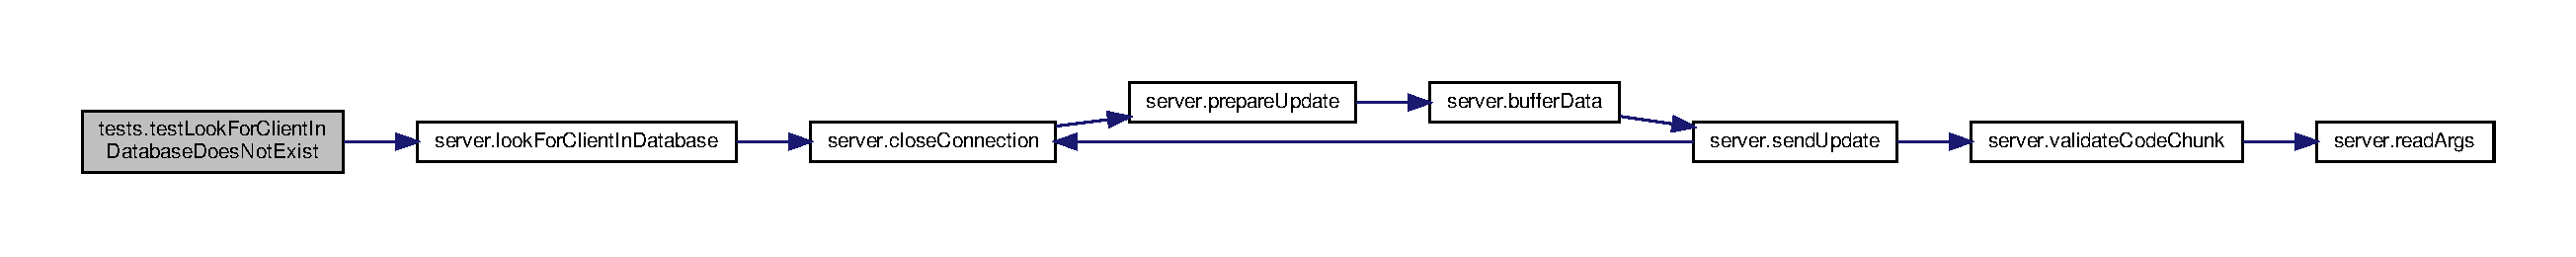
\includegraphics[width=350pt]{namespacetests_aa01c1b55c064d435f5ce63b79f8042a5_cgraph}
\end{center}
\end{figure}
Here is the caller graph for this function\+:
\nopagebreak
\begin{figure}[H]
\begin{center}
\leavevmode
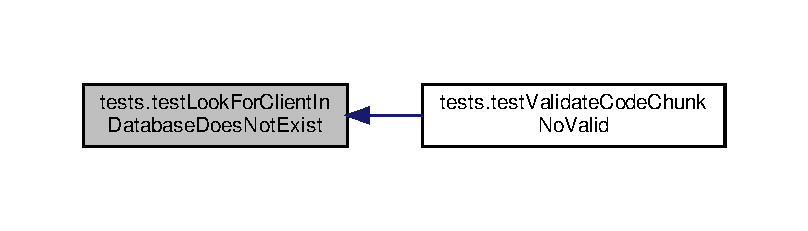
\includegraphics[width=350pt]{namespacetests_aa01c1b55c064d435f5ce63b79f8042a5_icgraph}
\end{center}
\end{figure}
\mbox{\Hypertarget{namespacetests_ab9d8846c7694143044a37e86e9447600}\label{namespacetests_ab9d8846c7694143044a37e86e9447600}} 
\index{tests@{tests}!test\+Look\+For\+Client\+In\+Database\+Exist@{test\+Look\+For\+Client\+In\+Database\+Exist}}
\index{test\+Look\+For\+Client\+In\+Database\+Exist@{test\+Look\+For\+Client\+In\+Database\+Exist}!tests@{tests}}
\subsubsection{\texorpdfstring{test\+Look\+For\+Client\+In\+Database\+Exist()}{testLookForClientInDatabaseExist()}}
{\footnotesize\ttfamily def tests.\+test\+Look\+For\+Client\+In\+Database\+Exist (\begin{DoxyParamCaption}{ }\end{DoxyParamCaption})}


\begin{DoxyCode}
5 \textcolor{keyword}{def }\hyperlink{namespacetests_ab9d8846c7694143044a37e86e9447600}{testLookForClientInDatabaseExist}():
6      mcuid = \textcolor{stringliteral}{"0001100023593110965955141"}
7      clientInfo = []
8      \textcolor{keywordflow}{if} (\hyperlink{namespaceserver_a998e5671e2ab0c79b9abe44e87e203a0}{server.lookForClientInDatabase}(mcuid, clientInfo) == 
      server.SUCCESSFUL):
9           server.printDebugL1(\textcolor{stringliteral}{"Successful test"})
10      \textcolor{keywordflow}{else}:
11           server.printDebugL1(\textcolor{stringliteral}{"Unsuccessfull test"})
12 
\end{DoxyCode}
Here is the call graph for this function\+:
\nopagebreak
\begin{figure}[H]
\begin{center}
\leavevmode
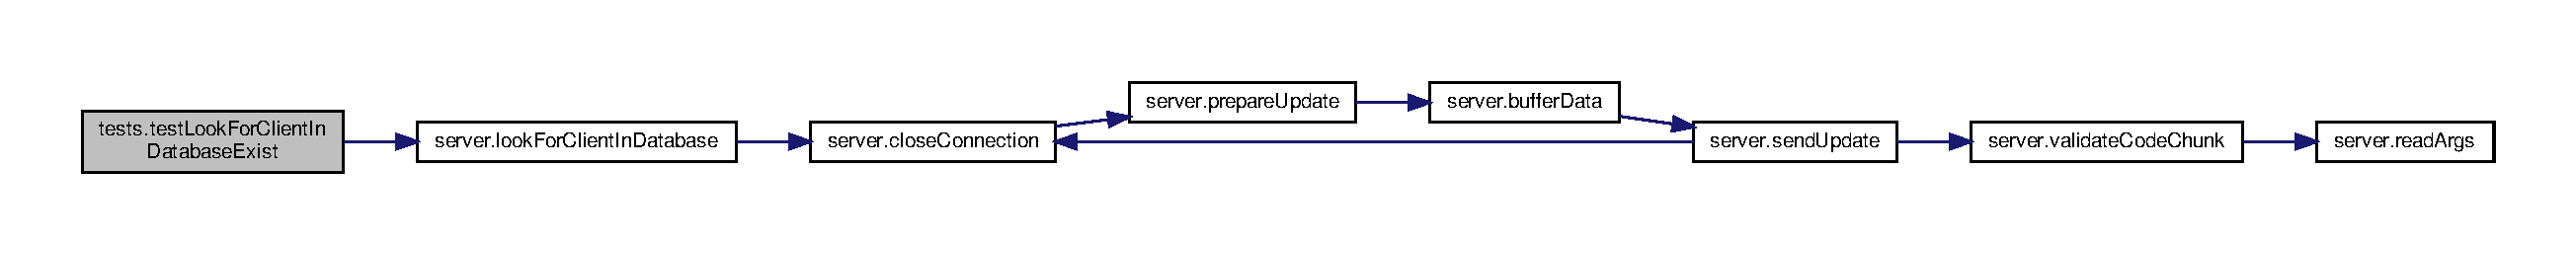
\includegraphics[width=350pt]{namespacetests_ab9d8846c7694143044a37e86e9447600_cgraph}
\end{center}
\end{figure}
Here is the caller graph for this function\+:
\nopagebreak
\begin{figure}[H]
\begin{center}
\leavevmode
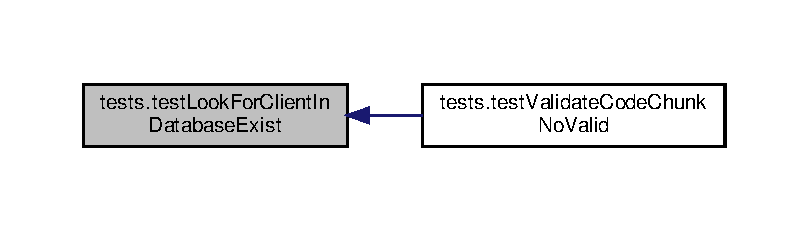
\includegraphics[width=350pt]{namespacetests_ab9d8846c7694143044a37e86e9447600_icgraph}
\end{center}
\end{figure}
\mbox{\Hypertarget{namespacetests_a1305f09454544d106db05e825d2ae813}\label{namespacetests_a1305f09454544d106db05e825d2ae813}} 
\index{tests@{tests}!test\+Prepare\+Update\+Non\+Existing\+Client@{test\+Prepare\+Update\+Non\+Existing\+Client}}
\index{test\+Prepare\+Update\+Non\+Existing\+Client@{test\+Prepare\+Update\+Non\+Existing\+Client}!tests@{tests}}
\subsubsection{\texorpdfstring{test\+Prepare\+Update\+Non\+Existing\+Client()}{testPrepareUpdateNonExistingClient()}}
{\footnotesize\ttfamily def tests.\+test\+Prepare\+Update\+Non\+Existing\+Client (\begin{DoxyParamCaption}{ }\end{DoxyParamCaption})}


\begin{DoxyCode}
21 \textcolor{keyword}{def }\hyperlink{namespacetests_a1305f09454544d106db05e825d2ae813}{testPrepareUpdateNonExistingClient}():
22      clientInfo = [\textcolor{stringliteral}{'0001100023593110965955141'},\textcolor{stringliteral}{'AN2295\_TWR\_K60.S19'},\textcolor{stringliteral}{'16'}]
23      clientsList= []
24      \textcolor{keywordflow}{if} (\hyperlink{namespaceserver_a4ab7e63c5f934dfea50b006468f9efca}{server.prepareUpdate}(clientInfo, clientsList) == server.SUCCESSFUL):
25           server.printDebugL1(\textcolor{stringliteral}{"\{\} Successful test"}.format(testPrepareUpdateNonExistingClient.\_\_name\_\_))
26      \textcolor{keywordflow}{else}:
27           server.printDebugL1(\textcolor{stringliteral}{"\{\} Unsuccessful test"}.format(testPrepareUpdateNonExistingClient.\_\_name\_\_))
28 
\end{DoxyCode}
Here is the call graph for this function\+:
\nopagebreak
\begin{figure}[H]
\begin{center}
\leavevmode
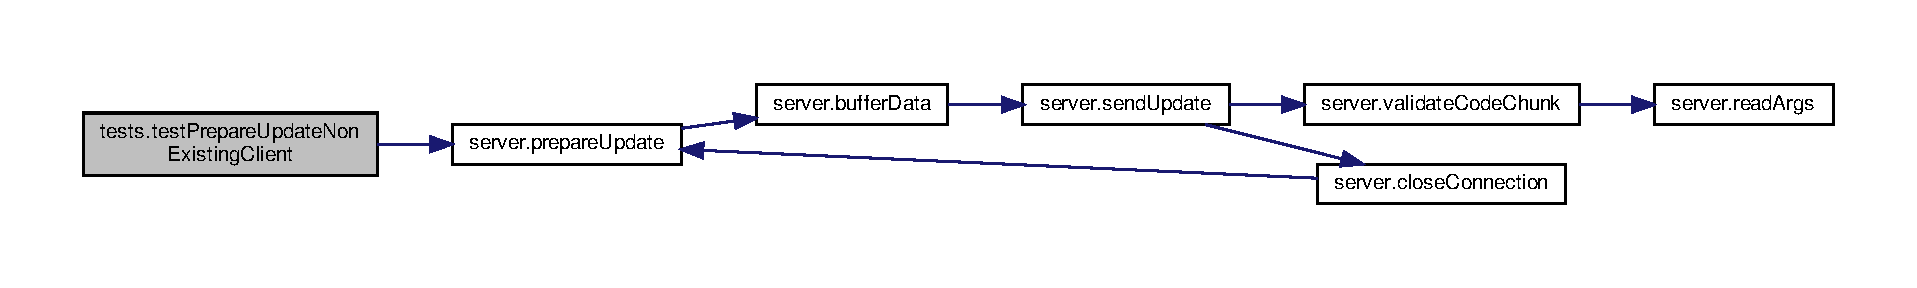
\includegraphics[width=350pt]{namespacetests_a1305f09454544d106db05e825d2ae813_cgraph}
\end{center}
\end{figure}
Here is the caller graph for this function\+:
\nopagebreak
\begin{figure}[H]
\begin{center}
\leavevmode
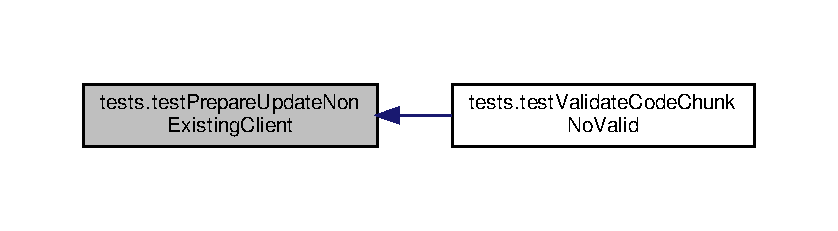
\includegraphics[width=350pt]{namespacetests_a1305f09454544d106db05e825d2ae813_icgraph}
\end{center}
\end{figure}
\mbox{\Hypertarget{namespacetests_a257095677e195c3499fa13fb7eb08a3e}\label{namespacetests_a257095677e195c3499fa13fb7eb08a3e}} 
\index{tests@{tests}!test\+Validate\+Code\+Chunk\+Empty@{test\+Validate\+Code\+Chunk\+Empty}}
\index{test\+Validate\+Code\+Chunk\+Empty@{test\+Validate\+Code\+Chunk\+Empty}!tests@{tests}}
\subsubsection{\texorpdfstring{test\+Validate\+Code\+Chunk\+Empty()}{testValidateCodeChunkEmpty()}}
{\footnotesize\ttfamily def tests.\+test\+Validate\+Code\+Chunk\+Empty (\begin{DoxyParamCaption}{ }\end{DoxyParamCaption})}


\begin{DoxyCode}
29 \textcolor{keyword}{def }\hyperlink{namespacetests_a257095677e195c3499fa13fb7eb08a3e}{testValidateCodeChunkEmpty}():
30      codechunk = \textcolor{stringliteral}{""}
31      \textcolor{keywordflow}{if} (\hyperlink{namespaceserver_ad6f5a9a8c8e233d0537dc69dc6de98f6}{server.validateCodeChunk}(codechunk) == server.INVALID\_CODE\_CHUNK):
32           server.printDebugL1(\textcolor{stringliteral}{"ChunkEmpty Successful test"})
33      \textcolor{keywordflow}{else}:
34           server.printDebugL1(\textcolor{stringliteral}{"ChunkEmpty Unsuccessful test"})
35 
\end{DoxyCode}
Here is the call graph for this function\+:
\nopagebreak
\begin{figure}[H]
\begin{center}
\leavevmode
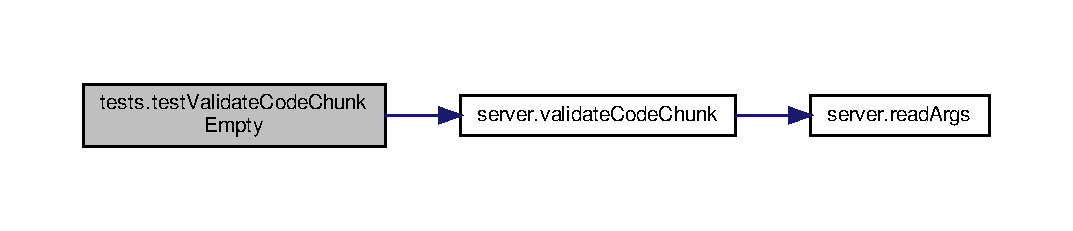
\includegraphics[width=350pt]{namespacetests_a257095677e195c3499fa13fb7eb08a3e_cgraph}
\end{center}
\end{figure}
Here is the caller graph for this function\+:
\nopagebreak
\begin{figure}[H]
\begin{center}
\leavevmode
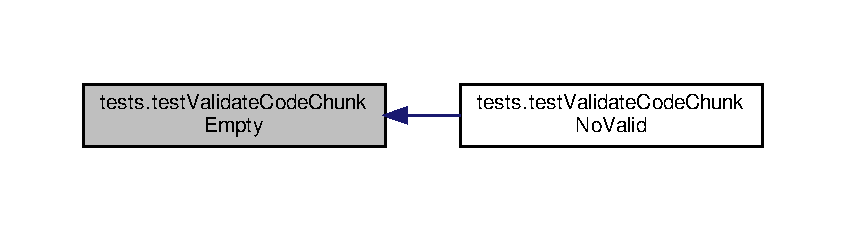
\includegraphics[width=350pt]{namespacetests_a257095677e195c3499fa13fb7eb08a3e_icgraph}
\end{center}
\end{figure}
\mbox{\Hypertarget{namespacetests_a625a9a5cd2f728455da250e9ba37d457}\label{namespacetests_a625a9a5cd2f728455da250e9ba37d457}} 
\index{tests@{tests}!test\+Validate\+Code\+Chunk\+No\+Valid@{test\+Validate\+Code\+Chunk\+No\+Valid}}
\index{test\+Validate\+Code\+Chunk\+No\+Valid@{test\+Validate\+Code\+Chunk\+No\+Valid}!tests@{tests}}
\subsubsection{\texorpdfstring{test\+Validate\+Code\+Chunk\+No\+Valid()}{testValidateCodeChunkNoValid()}}
{\footnotesize\ttfamily def tests.\+test\+Validate\+Code\+Chunk\+No\+Valid (\begin{DoxyParamCaption}{ }\end{DoxyParamCaption})}


\begin{DoxyCode}
43 \textcolor{keyword}{def }\hyperlink{namespacetests_a625a9a5cd2f728455da250e9ba37d457}{testValidateCodeChunkNoValid}():
44      codechunk = \textcolor{stringliteral}{"S786969"}
45      \textcolor{keywordflow}{if} (\hyperlink{namespaceserver_ad6f5a9a8c8e233d0537dc69dc6de98f6}{server.validateCodeChunk}(codechunk) == server.INVALID\_CODE\_CHUNK):
46           server.printDebugL1(\textcolor{stringliteral}{"ChunkNoValid Successful test"})
47      \textcolor{keywordflow}{else}:
48           server.printDebugL1(\textcolor{stringliteral}{"ChunkNoValid Unsuccessful test"})
49           
\end{DoxyCode}
Here is the call graph for this function\+:
\nopagebreak
\begin{figure}[H]
\begin{center}
\leavevmode
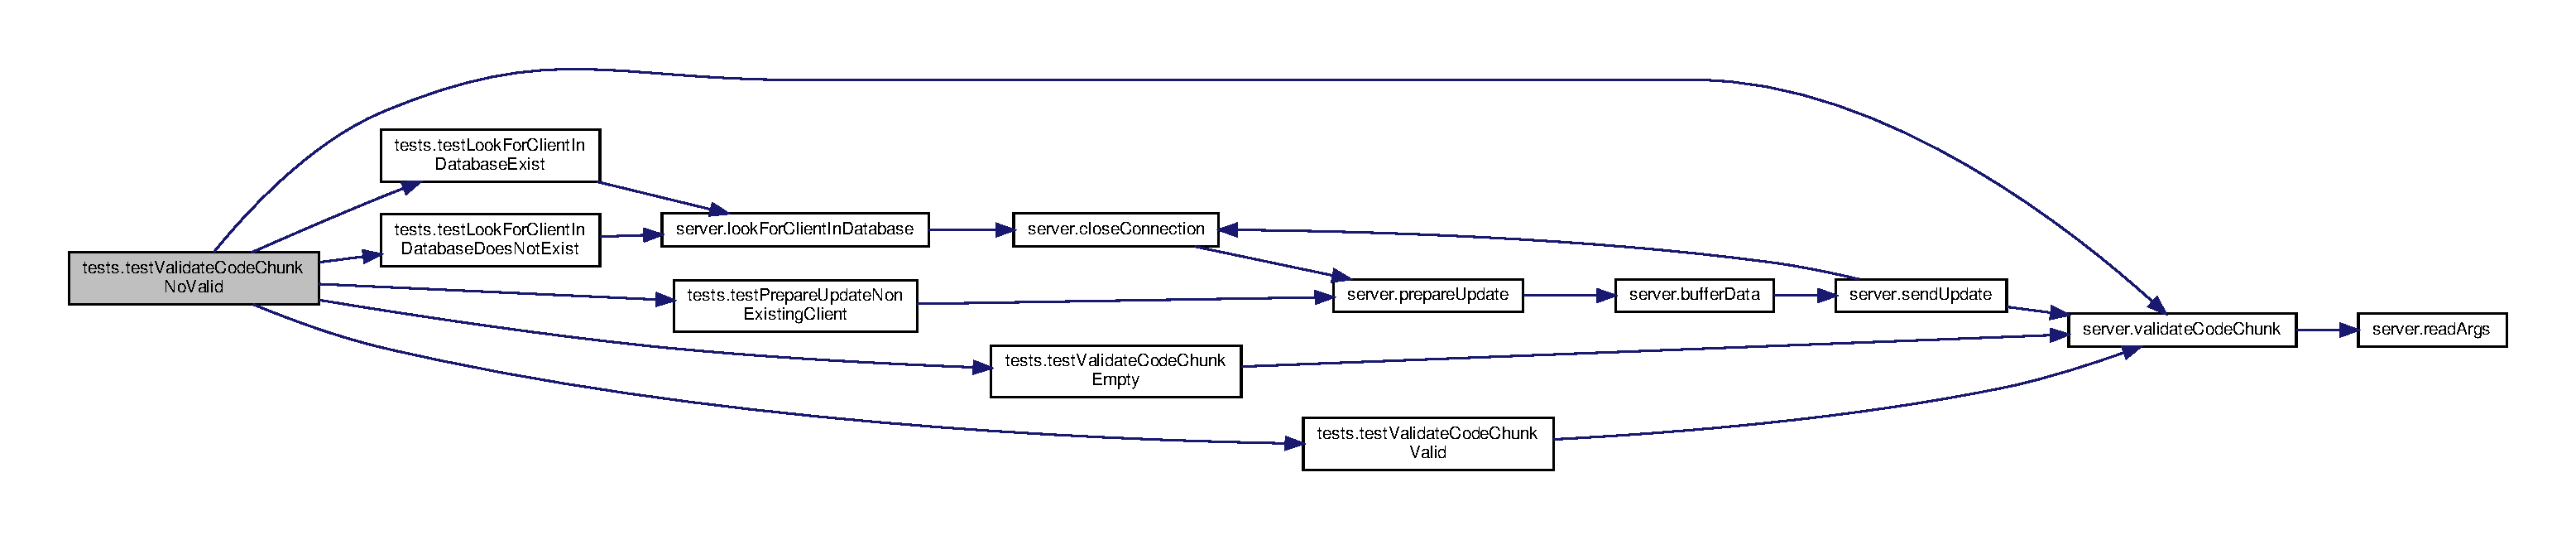
\includegraphics[width=350pt]{namespacetests_a625a9a5cd2f728455da250e9ba37d457_cgraph}
\end{center}
\end{figure}
\mbox{\Hypertarget{namespacetests_a4d364f808ece8a89192b5fa6bd230906}\label{namespacetests_a4d364f808ece8a89192b5fa6bd230906}} 
\index{tests@{tests}!test\+Validate\+Code\+Chunk\+Valid@{test\+Validate\+Code\+Chunk\+Valid}}
\index{test\+Validate\+Code\+Chunk\+Valid@{test\+Validate\+Code\+Chunk\+Valid}!tests@{tests}}
\subsubsection{\texorpdfstring{test\+Validate\+Code\+Chunk\+Valid()}{testValidateCodeChunkValid()}}
{\footnotesize\ttfamily def tests.\+test\+Validate\+Code\+Chunk\+Valid (\begin{DoxyParamCaption}{ }\end{DoxyParamCaption})}


\begin{DoxyCode}
36 \textcolor{keyword}{def }\hyperlink{namespacetests_a4d364f808ece8a89192b5fa6bd230906}{testValidateCodeChunkValid}():
37      codechunk = \textcolor{stringliteral}{"S197AAKA9779"}
38      \textcolor{keywordflow}{if} (\hyperlink{namespaceserver_ad6f5a9a8c8e233d0537dc69dc6de98f6}{server.validateCodeChunk}(codechunk) == server.SUCCESSFUL):
39           server.printDebugL1(\textcolor{stringliteral}{"ChunkValid Successful test"})
40      \textcolor{keywordflow}{else}:
41           server.printDebugL1(\textcolor{stringliteral}{"ChunkValid Unsuccessful test"})
42 
\end{DoxyCode}
Here is the call graph for this function\+:
\nopagebreak
\begin{figure}[H]
\begin{center}
\leavevmode
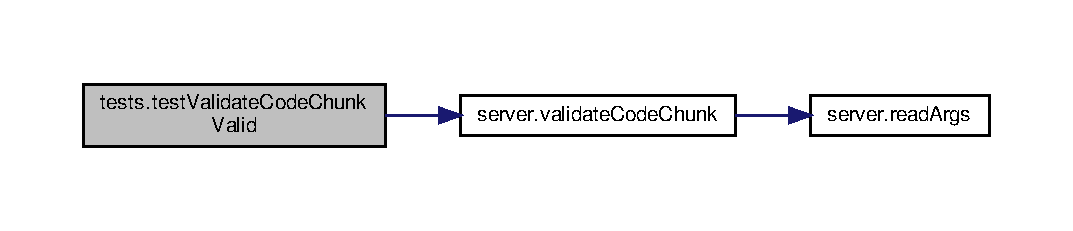
\includegraphics[width=350pt]{namespacetests_a4d364f808ece8a89192b5fa6bd230906_cgraph}
\end{center}
\end{figure}
Here is the caller graph for this function\+:
\nopagebreak
\begin{figure}[H]
\begin{center}
\leavevmode
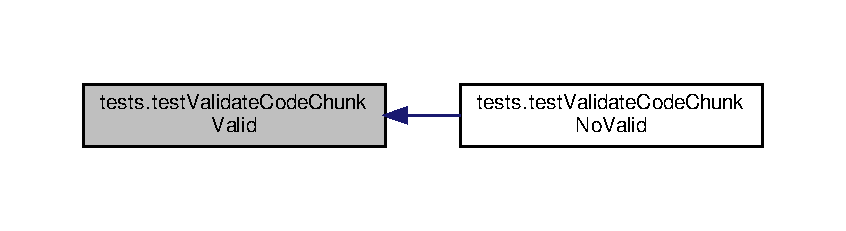
\includegraphics[width=350pt]{namespacetests_a4d364f808ece8a89192b5fa6bd230906_icgraph}
\end{center}
\end{figure}

\chapter{Class Documentation}
\hypertarget{classcustomlogger_1_1CustomLogger}{}\section{customlogger.\+Custom\+Logger Class Reference}
\label{classcustomlogger_1_1CustomLogger}\index{customlogger.\+Custom\+Logger@{customlogger.\+Custom\+Logger}}


Inheritance diagram for customlogger.\+Custom\+Logger\+:
\nopagebreak
\begin{figure}[H]
\begin{center}
\leavevmode
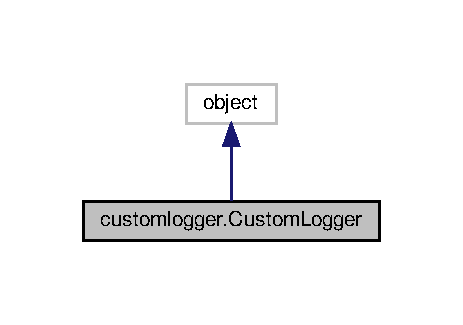
\includegraphics[width=222pt]{classcustomlogger_1_1CustomLogger__inherit__graph}
\end{center}
\end{figure}


Collaboration diagram for customlogger.\+Custom\+Logger\+:
\nopagebreak
\begin{figure}[H]
\begin{center}
\leavevmode
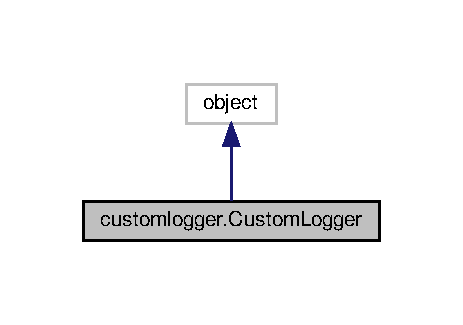
\includegraphics[width=222pt]{classcustomlogger_1_1CustomLogger__coll__graph}
\end{center}
\end{figure}
\subsection*{Public Member Functions}
\begin{DoxyCompactItemize}
\item 
def \hyperlink{classcustomlogger_1_1CustomLogger_ad0fa3a11a371fa6b445768b0b9e8fe03}{\+\_\+\+\_\+init\+\_\+\+\_\+} (self, \hyperlink{classcustomlogger_1_1CustomLogger_a800aa033e5fd2a8fc1e108a6046fd7fe}{logger}, \hyperlink{classcustomlogger_1_1CustomLogger_aa1e8b5f7e7dd6b9a1c2db6e66f3c3da6}{level})
\item 
def \hyperlink{classcustomlogger_1_1CustomLogger_ae4e52add9e53df464b370744233b16f7}{write} (self, message)
\end{DoxyCompactItemize}
\subsection*{Public Attributes}
\begin{DoxyCompactItemize}
\item 
\hyperlink{classcustomlogger_1_1CustomLogger_a800aa033e5fd2a8fc1e108a6046fd7fe}{logger}
\item 
\hyperlink{classcustomlogger_1_1CustomLogger_aa1e8b5f7e7dd6b9a1c2db6e66f3c3da6}{level}
\end{DoxyCompactItemize}


\subsection{Constructor \& Destructor Documentation}
\mbox{\Hypertarget{classcustomlogger_1_1CustomLogger_ad0fa3a11a371fa6b445768b0b9e8fe03}\label{classcustomlogger_1_1CustomLogger_ad0fa3a11a371fa6b445768b0b9e8fe03}} 
\index{customlogger\+::\+Custom\+Logger@{customlogger\+::\+Custom\+Logger}!\+\_\+\+\_\+init\+\_\+\+\_\+@{\+\_\+\+\_\+init\+\_\+\+\_\+}}
\index{\+\_\+\+\_\+init\+\_\+\+\_\+@{\+\_\+\+\_\+init\+\_\+\+\_\+}!customlogger\+::\+Custom\+Logger@{customlogger\+::\+Custom\+Logger}}
\subsubsection{\texorpdfstring{\+\_\+\+\_\+init\+\_\+\+\_\+()}{\_\_init\_\_()}}
{\footnotesize\ttfamily def customlogger.\+Custom\+Logger.\+\_\+\+\_\+init\+\_\+\+\_\+ (\begin{DoxyParamCaption}\item[{}]{self,  }\item[{}]{logger,  }\item[{}]{level }\end{DoxyParamCaption})}


\begin{DoxyCode}
9      \textcolor{keyword}{def }\_\_init\_\_(self, logger, level):
10           \textcolor{comment}{#Needs a logger and a logger level}
11           self.logger = logger
12           self.level = level
13           
\end{DoxyCode}


\subsection{Member Function Documentation}
\mbox{\Hypertarget{classcustomlogger_1_1CustomLogger_ae4e52add9e53df464b370744233b16f7}\label{classcustomlogger_1_1CustomLogger_ae4e52add9e53df464b370744233b16f7}} 
\index{customlogger\+::\+Custom\+Logger@{customlogger\+::\+Custom\+Logger}!write@{write}}
\index{write@{write}!customlogger\+::\+Custom\+Logger@{customlogger\+::\+Custom\+Logger}}
\subsubsection{\texorpdfstring{write()}{write()}}
{\footnotesize\ttfamily def customlogger.\+Custom\+Logger.\+write (\begin{DoxyParamCaption}\item[{}]{self,  }\item[{}]{message }\end{DoxyParamCaption})}


\begin{DoxyCode}
14      \textcolor{keyword}{def }write(self, message):
15           \textcolor{comment}{#Only log if there is a message (not just a new line)}
16           \textcolor{keywordflow}{if} message.rstrip() != \textcolor{stringliteral}{""}:
17                self.logger.log(self.level, message.rstrip())
18 \end{DoxyCode}


\subsection{Member Data Documentation}
\mbox{\Hypertarget{classcustomlogger_1_1CustomLogger_aa1e8b5f7e7dd6b9a1c2db6e66f3c3da6}\label{classcustomlogger_1_1CustomLogger_aa1e8b5f7e7dd6b9a1c2db6e66f3c3da6}} 
\index{customlogger\+::\+Custom\+Logger@{customlogger\+::\+Custom\+Logger}!level@{level}}
\index{level@{level}!customlogger\+::\+Custom\+Logger@{customlogger\+::\+Custom\+Logger}}
\subsubsection{\texorpdfstring{level}{level}}
{\footnotesize\ttfamily customlogger.\+Custom\+Logger.\+level}

\mbox{\Hypertarget{classcustomlogger_1_1CustomLogger_a800aa033e5fd2a8fc1e108a6046fd7fe}\label{classcustomlogger_1_1CustomLogger_a800aa033e5fd2a8fc1e108a6046fd7fe}} 
\index{customlogger\+::\+Custom\+Logger@{customlogger\+::\+Custom\+Logger}!logger@{logger}}
\index{logger@{logger}!customlogger\+::\+Custom\+Logger@{customlogger\+::\+Custom\+Logger}}
\subsubsection{\texorpdfstring{logger}{logger}}
{\footnotesize\ttfamily customlogger.\+Custom\+Logger.\+logger}



The documentation for this class was generated from the following file\+:\begin{DoxyCompactItemize}
\item 
\hyperlink{customlogger_8py}{customlogger.\+py}\end{DoxyCompactItemize}

\chapter{File Documentation}
\hypertarget{customlogger_8py}{}\section{customlogger.\+py File Reference}
\label{customlogger_8py}\index{customlogger.\+py@{customlogger.\+py}}
\subsection*{Classes}
\begin{DoxyCompactItemize}
\item 
class \hyperlink{classcustomlogger_1_1CustomLogger}{customlogger.\+Custom\+Logger}
\end{DoxyCompactItemize}
\subsection*{Namespaces}
\begin{DoxyCompactItemize}
\item 
 \hyperlink{namespacecustomlogger}{customlogger}
\end{DoxyCompactItemize}

\hypertarget{README_8md}{}\section{R\+E\+A\+D\+M\+E.\+md File Reference}
\label{README_8md}\index{R\+E\+A\+D\+M\+E.\+md@{R\+E\+A\+D\+M\+E.\+md}}

\hypertarget{server_8py}{}\section{server.\+py File Reference}
\label{server_8py}\index{server.\+py@{server.\+py}}
\subsection*{Namespaces}
\begin{DoxyCompactItemize}
\item 
 \hyperlink{namespaceserver}{server}
\item 
 \hyperlink{namespaceServer_1_1py}{Server.\+py}
\begin{DoxyCompactList}\small\item\em Create a server and enable R\+E\+ST A\+PI for firmware updates. \end{DoxyCompactList}\end{DoxyCompactItemize}
\subsection*{Functions}
\begin{DoxyCompactItemize}
\item 
def \hyperlink{namespaceserver_aa317dc86338d02253076787cc8e5d997}{server.\+read\+Args} ()
\item 
def \hyperlink{namespaceserver_a44a7428717edc164d7dd564478da2da3}{server.\+configure\+Logger} (log\+File)
\item 
def \hyperlink{namespaceserver_a240f07b12d57cfa5cff5612501fe7dc8}{server.\+create\+Server} (connections\+List, clients\+List)
\item 
def \hyperlink{namespaceserver_ac1ec62c626a3425033381ef5718ce12b}{server.\+accept\+Connections} (connections\+List, clients\+List, sock, logger)
\item 
def \hyperlink{namespaceserver_a4e6504daf55d2ef34d4d2ea5b30074f3}{server.\+verify\+Started\+Connection} (connections, connection)
\item 
def \hyperlink{namespaceserver_a26f3a1d49ee9e013ed77fbcb273a99be}{server.\+get\+M\+C\+U\+ID} (connection, address, logger)
\item 
def \hyperlink{namespaceserver_a4c51be10ba9f982375f4c0a426078a96}{server.\+verify\+Client\+Id} (connection, mcuid, logger)
\item 
def \hyperlink{namespaceserver_a998e5671e2ab0c79b9abe44e87e203a0}{server.\+look\+For\+Client\+In\+Database} (mcuid, logger)
\item 
def \hyperlink{namespaceserver_a2e99d18201fed087163454b021b7c007}{server.\+close\+Connection} (connection, logger)
\item 
def \hyperlink{namespaceserver_a4ab7e63c5f934dfea50b006468f9efca}{server.\+prepare\+Update} (client\+Info, clients\+List, logger)
\item 
def \hyperlink{namespaceserver_a6098d5cffff301a01e793c84215c4512}{server.\+buffer\+Data} (filename, binary\+File\+Lines, logger)
\item 
def \hyperlink{namespaceserver_a4889d0db3f3503cc61340252fabc2c24}{server.\+send\+Update} (connection, address, mcuid, client\+To\+Update, sock, logger)
\item 
def \hyperlink{namespaceserver_ad6f5a9a8c8e233d0537dc69dc6de98f6}{server.\+validate\+Code\+Chunk} (codechunk)
\end{DoxyCompactItemize}
\subsection*{Variables}
\begin{DoxyCompactItemize}
\item 
int \hyperlink{namespaceserver_a3ae1ac2f6b7f0e83705066a294c6af9b}{server.\+D\+E\+B\+U\+G\+\_\+\+ON} = 1
\begin{DoxyCompactList}\small\item\em Enable 1 Disable 0 Debug. \end{DoxyCompactList}\item 
string \hyperlink{namespaceserver_a6e3160a2459a5f5c0b05d31bea269c07}{server.\+L\+O\+G\+\_\+\+P\+A\+T\+H\+\_\+\+D\+E\+F\+A\+U\+LT} = \char`\"{}/tmp\char`\"{}
\begin{DoxyCompactList}\small\item\em Defaults files to log. \end{DoxyCompactList}\item 
string \hyperlink{namespaceserver_ae9611c1fa51131280e6b7c2e7ea199af}{server.\+L\+O\+G\+\_\+\+F\+I\+L\+E\+N\+A\+M\+E\+\_\+\+D\+E\+F\+A\+U\+LT} = \char`\"{}/otaserver.\+log\char`\"{}
\item 
\hyperlink{namespaceserver_a623756b923995322c8ea575f3b9e70ba}{server.\+L\+O\+G\+\_\+\+L\+E\+V\+EL} = logging.\+I\+N\+FO
\item 
int \hyperlink{namespaceserver_ac636d4745eb8df94294d20a79e9736c2}{server.\+S\+U\+C\+C\+E\+S\+S\+F\+UL} = 0
\item 
int \hyperlink{namespaceserver_aa1f32b90430e9bda83de3d5e601402d5}{server.\+C\+L\+I\+E\+N\+T\+\_\+\+U\+N\+V\+E\+R\+I\+F\+I\+ED} = 1
\item 
int \hyperlink{namespaceserver_abd54d09502b28ddf1b7c67d7128f0770}{server.\+M\+I\+S\+S\+E\+D\+\_\+\+F\+I\+L\+E\+N\+A\+ME} = 2
\item 
int \hyperlink{namespaceserver_ae93172172b034664ce8a47255943b867}{server.\+U\+N\+F\+O\+R\+M\+A\+T\+T\+E\+D\+\_\+\+M\+C\+U\+ID} = 3
\item 
int \hyperlink{namespaceserver_a02bffbe3ff309c8cca6cfdc9fe84b335}{server.\+A\+L\+R\+E\+A\+D\+Y\+\_\+\+S\+T\+A\+R\+T\+E\+D\+\_\+\+C\+O\+N\+N\+E\+C\+T\+I\+ON} = 4
\item 
int \hyperlink{namespaceserver_ac3607b92a19b8b6e55eec69cd0e45e6d}{server.\+N\+O\+T\+\_\+\+S\+T\+A\+R\+T\+E\+D\+\_\+\+C\+O\+N\+N\+E\+C\+T\+I\+ON} = 4
\item 
int \hyperlink{namespaceserver_a6d2a5626a7ca491da6005e14db1de116}{server.\+U\+N\+A\+B\+L\+E\+\_\+\+B\+U\+F\+F\+E\+R\+I\+N\+G\+\_\+\+C\+O\+DE} = 5
\item 
int \hyperlink{namespaceserver_ae355ef915b96ba835f2a760f4b441679}{server.\+U\+N\+P\+R\+O\+P\+E\+R\+\_\+\+F\+I\+L\+E\+\_\+\+F\+O\+R\+M\+AT} = 6
\item 
int \hyperlink{namespaceserver_a91d094730b5907a9e14d0f4098b490b9}{server.\+T\+I\+M\+E\+O\+U\+T\+\_\+\+C\+O\+N\+N\+E\+C\+T\+I\+ON} = 7
\item 
int \hyperlink{namespaceserver_a4782abb5e785dbf608b8b8d553bbac12}{server.\+I\+N\+V\+A\+L\+I\+D\+\_\+\+C\+O\+D\+E\+\_\+\+C\+H\+U\+NK} = 8
\item 
int \hyperlink{namespaceserver_aabc8079ca922bed2eba00ad2cbc5d354}{server.\+B\+U\+F\+F\+E\+R\+I\+N\+G\+\_\+\+C\+O\+D\+E\+\_\+\+I\+N\+C\+O\+M\+P\+L\+E\+TE} = 9
\item 
int \hyperlink{namespaceserver_a1da647756067c40eea52b91451e82ad5}{server.\+R\+E\+A\+D\+Y\+\_\+\+T\+O\+\_\+\+U\+P\+D\+A\+TE} = 10
\item 
int \hyperlink{namespaceserver_abcf4d8f2c33b95345413f5e15c24a01e}{server.\+T\+I\+M\+E\+O\+UT} = 30
\item 
string \hyperlink{namespaceserver_abad27332b11c625d6b59b5fc1ca4b2b2}{server.\+H\+O\+S\+T\+\_\+\+D\+E\+F\+A\+U\+LT} = \textquotesingle{}\textquotesingle{}
\item 
int \hyperlink{namespaceserver_aa0fba16fbbcb0260d63ddce950cecb42}{server.\+P\+O\+R\+T\+\_\+\+D\+E\+F\+A\+U\+LT} = 4000
\item 
string \hyperlink{namespaceserver_a064d84330983ae4788826100a0238c78}{server.\+P\+A\+T\+H\+\_\+\+B\+I\+N\+A\+R\+Y\+\_\+\+F\+I\+L\+E\+\_\+\+D\+E\+F\+A\+U\+LT} = \char`\"{}/root/fota/otaserver/bin\char`\"{}
\item 
string \hyperlink{namespaceserver_aa3f9ad91c62b5372a5e677c50b853605}{server.\+P\+A\+T\+H\+\_\+\+D\+A\+T\+A\+B\+A\+S\+E\+\_\+\+D\+E\+F\+A\+U\+LT} = \char`\"{}/root/fota/otaserver/database/devices2update.\+txt\char`\"{}
\item 
string \hyperlink{namespaceserver_a097162d68fd6d2855bf5eb81507db414}{server.\+allowed\+Update} = b\textquotesingle{}@4\#\textquotesingle{}
\item 
string \hyperlink{namespaceserver_ae86ca5f489b3b8161c0ab91cbef0d8e6}{server.\+banned\+Update} = b\textquotesingle{}@0\#\textquotesingle{}
\item 
string \hyperlink{namespaceserver_ad00458dfe9ab743680203b756f8345bf}{server.\+ack\+Client} = b\textquotesingle{}@\textquotesingle{}
\item 
int \hyperlink{namespaceserver_a49c2646e7b6a517fe077d830219c58d4}{server.\+buffer\+Size\+File} = 300
\item 
int \hyperlink{namespaceserver_a100b5332a3005033a437d4240302698d}{server.\+max\+Bytes} = 1024
\item 
string \hyperlink{namespaceserver_a34ef43a269b2139fb82ac42e3d9e525a}{server.\+path\+Binary\+Files} = \char`\"{}\char`\"{}
\item 
string \hyperlink{namespaceserver_ad56bacd311418978d78a8d1467a221a0}{server.\+database\+Name} = \char`\"{}\char`\"{}
\item 
string \hyperlink{namespaceserver_a4230afe85d97e78a1df6181d40cbe0b7}{server.\+host} = \char`\"{}\char`\"{}
\item 
string \hyperlink{namespaceserver_accc83f0ac9fb96c740cb3df16517e927}{server.\+port} = \char`\"{}\char`\"{}
\item 
string \hyperlink{namespaceserver_a45d593b7c621a117aaef105bf59d9fd5}{server.\+log\+Path} = \char`\"{}\char`\"{}
\item 
list \hyperlink{namespaceserver_acc620e319dd97213c1d3758ea4de7f68}{server.\+inputs} = \mbox{[}$\,$\mbox{]}
\item 
def \hyperlink{namespaceserver_aea7e1efc19535ee9bab8400a812b43a9}{server.\+args} = read\+Args()
\item 
string \hyperlink{namespaceserver_ab968a55cbe8af171a0fcbae9a876cab4}{server.\+log\+File} = log\+Path + L\+O\+G\+\_\+\+F\+I\+L\+E\+N\+A\+M\+E\+\_\+\+D\+E\+F\+A\+U\+LT
\item 
def \hyperlink{namespaceserver_abfa1d56012bc320e4b26361390f6fc24}{server.\+logger} = configure\+Logger(log\+File)
\item 
list \hyperlink{namespaceserver_a734e47a5cf907dc2e128358488a9c3e7}{server.\+connections\+List} = \mbox{[}$\,$\mbox{]}
\item 
list \hyperlink{namespaceserver_acc42864cdf2e6dd395c42dd780cbde1d}{server.\+clients\+List} = \mbox{[}$\,$\mbox{]}
\end{DoxyCompactItemize}

\hypertarget{tests_2parallelize_2multiprocessing_2server_8py}{}\section{tests/parallelize/multiprocessing/server.py File Reference}
\label{tests_2parallelize_2multiprocessing_2server_8py}\index{tests/parallelize/multiprocessing/server.\+py@{tests/parallelize/multiprocessing/server.\+py}}
\subsection*{Namespaces}
\begin{DoxyCompactItemize}
\item 
 \hyperlink{namespaceserver}{server}
\end{DoxyCompactItemize}
\subsection*{Functions}
\begin{DoxyCompactItemize}
\item 
def \hyperlink{namespaceserver_a5dce7c3abe85653dccf395dfb4f4b664}{server.\+connect\+Socket} (socket)
\end{DoxyCompactItemize}
\subsection*{Variables}
\begin{DoxyCompactItemize}
\item 
int \hyperlink{namespaceserver_a8f2c905b49be657a873ebe6d354d4b47}{server.\+M\+A\+X\+\_\+\+O\+P\+E\+N\+\_\+\+C\+O\+N\+N\+E\+C\+T\+I\+O\+NS} = 5
\item 
int \hyperlink{namespaceserver_ab9cbbed2baf7ef46dcd7d67fcb351ac7}{server.\+connected\+Clients} = 0
\item 
list \hyperlink{namespaceserver_a0d0a0c96488e0f2fb395618dd4658135}{server.\+open\+Connections} = \mbox{[}$\,$\mbox{]}
\item 
\hyperlink{namespaceserver_ae005445cadfc079ed27cd779020f5f32}{server.\+serversocket} = socket.\+socket (socket.\+A\+F\+\_\+\+I\+N\+ET, socket.\+S\+O\+C\+K\+\_\+\+S\+T\+R\+E\+AM)
\item 
\hyperlink{namespaceserver_a6c2bf59cef00216ae7fee937e55f013d}{server.\+target}
\item 
\hyperlink{namespaceserver_ace8bd717303af3e13cd4dba46b2cd5f1}{server.\+connect\+Socket}
\end{DoxyCompactItemize}

\hypertarget{tests_2parallelize_2selectApproach_2server_8py}{}\section{tests/parallelize/select\+Approach/server.py File Reference}
\label{tests_2parallelize_2selectApproach_2server_8py}\index{tests/parallelize/select\+Approach/server.\+py@{tests/parallelize/select\+Approach/server.\+py}}
\subsection*{Namespaces}
\begin{DoxyCompactItemize}
\item 
 \hyperlink{namespaceserver}{server}
\end{DoxyCompactItemize}
\subsection*{Variables}
\begin{DoxyCompactItemize}
\item 
\hyperlink{namespaceserver_a995df52292d049e26620aefae8eb4e1d}{server.\+sock} = socket.\+socket(socket.\+A\+F\+\_\+\+I\+N\+ET, socket.\+S\+O\+C\+K\+\_\+\+S\+T\+R\+E\+AM)
\item 
list \hyperlink{namespaceserver_af6312e19169c5addc1dafc4954287d67}{server.\+outputs} = \mbox{[}$\,$\mbox{]}
\item 
list \hyperlink{namespaceserver_a8a14948c5211d04b3a2b33b730b991b2}{server.\+excepts} = \mbox{[}$\,$\mbox{]}
\item 
\hyperlink{namespaceserver_accef440b565edfb162319da0f775b284}{server.\+readable}
\item 
\hyperlink{namespaceserver_accc7fda5853169f8f74f25dfb423b576}{server.\+writable}
\item 
\hyperlink{namespaceserver_aa9a1622b227ab6db4b65781454c92504}{server.\+exceptional}
\item 
\hyperlink{namespaceserver_ab8d0bbcdb7423e60b0d370a6d21a1781}{server.\+clientsock}
\item 
\hyperlink{namespaceserver_a90279b585d4f187d0908de4962d5cb8d}{server.\+clientaddr}
\item 
\hyperlink{namespaceserver_a8b7790a9997c09aa90cf4a121a310d5c}{server.\+data} = readable\+Socket.\+recv(1024)
\end{DoxyCompactItemize}

\hypertarget{client_8py}{}\section{tests/client.py File Reference}
\label{client_8py}\index{tests/client.\+py@{tests/client.\+py}}
\subsection*{Namespaces}
\begin{DoxyCompactItemize}
\item 
 \hyperlink{namespaceclient}{client}
\end{DoxyCompactItemize}
\subsection*{Functions}
\begin{DoxyCompactItemize}
\item 
def \hyperlink{namespaceclient_aa133740df708d11451616cdd39a08b91}{client.\+verify\+Finished\+Update} (data)
\end{DoxyCompactItemize}
\subsection*{Variables}
\begin{DoxyCompactItemize}
\item 
string \hyperlink{namespaceclient_a25ca49ee73998b47f449af9549f4634e}{client.\+ack\+Client} = b\char`\"{}@\char`\"{}
\item 
string \hyperlink{namespaceclient_a245a3a9a5536dcbb58fd7a83934854d3}{client.\+approved\+Update} = b\char`\"{}@4\#\char`\"{}
\item 
string \hyperlink{namespaceclient_ad39c4666bbab8c2e37b88274a0eaf7ba}{client.\+H\+O\+ST} = \textquotesingle{}209.\+97.\+145.\+137\textquotesingle{}
\item 
int \hyperlink{namespaceclient_acd2f280864b8945bb46e196ed2b0990a}{client.\+P\+O\+RT} = 4000
\item 
list \hyperlink{namespaceclient_abf9b35467956bfa36acd984aace33449}{client.\+binary\+Code} = \mbox{[}$\,$\mbox{]}
\item 
\hyperlink{namespaceclient_ad4a7c4191c3c65a9bdc2ac03d3464f13}{client.\+s} = socket.\+socket(socket.\+A\+F\+\_\+\+I\+N\+ET, socket.\+S\+O\+C\+K\+\_\+\+S\+T\+R\+E\+AM)
\item 
\hyperlink{namespaceclient_ade2c74246e97a6a8badb63b11888eb96}{client.\+data} = s.\+recv(1024)
\item 
def \hyperlink{namespaceclient_acb1b64fab7439cf2fdc191f31daa8353}{client.\+finished\+Update} = verify\+Finished\+Update(data)
\end{DoxyCompactItemize}

\hypertarget{parallelize_2selectApproach_2client_8py}{}\section{tests/parallelize/select\+Approach/client.py File Reference}
\label{parallelize_2selectApproach_2client_8py}\index{tests/parallelize/select\+Approach/client.\+py@{tests/parallelize/select\+Approach/client.\+py}}
\subsection*{Namespaces}
\begin{DoxyCompactItemize}
\item 
 \hyperlink{namespaceclient}{client}
\end{DoxyCompactItemize}
\subsection*{Variables}
\begin{DoxyCompactItemize}
\item 
int \hyperlink{namespaceclient_a1e07168544409bc8bf0b656eebc8e888}{client.\+T\+I\+M\+E\+O\+UT} = 5
\item 
string \hyperlink{namespaceclient_affd1b2de2616b92fa875ddb4f94f21a0}{client.\+host} = \textquotesingle{}127.\+0.\+0.\+1\textquotesingle{}
\item 
int \hyperlink{namespaceclient_ad13ec39ec5b973ae74c855e52b1e5652}{client.\+port} = 10000
\item 
\hyperlink{namespaceclient_ad8df363cc6c2fdd1e4f4f3b3d9d0c8fd}{client.\+sock} = socket.\+socket(socket.\+A\+F\+\_\+\+I\+N\+ET, socket.\+S\+O\+C\+K\+\_\+\+S\+T\+R\+E\+AM)
\item 
\hyperlink{namespaceclient_a09b2af09e6bb63b2b014637b5b4e2936}{client.\+buf} = sock.\+recv(1024)
\end{DoxyCompactItemize}

\hypertarget{NoClient_8py}{}\section{tests/\+No\+Client.py File Reference}
\label{NoClient_8py}\index{tests/\+No\+Client.\+py@{tests/\+No\+Client.\+py}}
\subsection*{Namespaces}
\begin{DoxyCompactItemize}
\item 
 \hyperlink{namespaceNoClient}{No\+Client}
\end{DoxyCompactItemize}
\subsection*{Functions}
\begin{DoxyCompactItemize}
\item 
def \hyperlink{namespaceNoClient_ac97f6af869f1514eb8ce4f1b205c2bd5}{No\+Client.\+verify\+Finished\+Update} (data)
\end{DoxyCompactItemize}
\subsection*{Variables}
\begin{DoxyCompactItemize}
\item 
string \hyperlink{namespaceNoClient_afa59067c297f089b96e52a26cbe65e35}{No\+Client.\+ack\+Client} = b\char`\"{}@\char`\"{}
\item 
string \hyperlink{namespaceNoClient_a8a8f39cca298d07544827e3e590155f4}{No\+Client.\+approved\+Update} = b\char`\"{}@4\#\char`\"{}
\item 
string \hyperlink{namespaceNoClient_a6f89bd992508c504035304f4773518d3}{No\+Client.\+H\+O\+ST} = \textquotesingle{}209.\+97.\+145.\+137\textquotesingle{}
\item 
int \hyperlink{namespaceNoClient_abb61c9ed514d4ed04b9689a37b40ee80}{No\+Client.\+P\+O\+RT} = 4000
\item 
list \hyperlink{namespaceNoClient_a40004afa65328c18891bec9feca29dad}{No\+Client.\+binary\+Code} = \mbox{[}$\,$\mbox{]}
\item 
\hyperlink{namespaceNoClient_a07aafa72fabaac63d60eb7397828e128}{No\+Client.\+s} = socket.\+socket(socket.\+A\+F\+\_\+\+I\+N\+ET, socket.\+S\+O\+C\+K\+\_\+\+S\+T\+R\+E\+AM)
\item 
\hyperlink{namespaceNoClient_a3687413639bcde5799ea49121c61206d}{No\+Client.\+data} = s.\+recv(1024)
\item 
def \hyperlink{namespaceNoClient_a408c6aa37feaeb4ce526cb6af66bdda2}{No\+Client.\+finished\+Update} = verify\+Finished\+Update(data)
\end{DoxyCompactItemize}

\hypertarget{tests_8py}{}\section{tests/tests.py File Reference}
\label{tests_8py}\index{tests/tests.\+py@{tests/tests.\+py}}
\subsection*{Namespaces}
\begin{DoxyCompactItemize}
\item 
 \hyperlink{namespacetests}{tests}
\end{DoxyCompactItemize}
\subsection*{Functions}
\begin{DoxyCompactItemize}
\item 
def \hyperlink{namespacetests_ab9d8846c7694143044a37e86e9447600}{tests.\+test\+Look\+For\+Client\+In\+Database\+Exist} ()
\item 
def \hyperlink{namespacetests_aa01c1b55c064d435f5ce63b79f8042a5}{tests.\+test\+Look\+For\+Client\+In\+Database\+Does\+Not\+Exist} ()
\item 
def \hyperlink{namespacetests_a1305f09454544d106db05e825d2ae813}{tests.\+test\+Prepare\+Update\+Non\+Existing\+Client} ()
\item 
def \hyperlink{namespacetests_a257095677e195c3499fa13fb7eb08a3e}{tests.\+test\+Validate\+Code\+Chunk\+Empty} ()
\item 
def \hyperlink{namespacetests_a4d364f808ece8a89192b5fa6bd230906}{tests.\+test\+Validate\+Code\+Chunk\+Valid} ()
\item 
def \hyperlink{namespacetests_a625a9a5cd2f728455da250e9ba37d457}{tests.\+test\+Validate\+Code\+Chunk\+No\+Valid} ()
\end{DoxyCompactItemize}

%--- End generated contents ---

% Index
\backmatter
\newpage
\phantomsection
\clearemptydoublepage
\addcontentsline{toc}{chapter}{Index}
\printindex

\end{document}
